% Generated by Sphinx.
\def\sphinxdocclass{report}
\documentclass[letterpaper,10pt,english]{sphinxmanual}
\usepackage[utf8]{inputenc}
\DeclareUnicodeCharacter{00A0}{\nobreakspace}
\usepackage[T1]{fontenc}
\usepackage{babel}
\usepackage{times}
\usepackage[Bjarne]{fncychap}
\usepackage{longtable}
\usepackage{sphinx}
\usepackage{multirow}


\title{Pythics Documentation}
\date{March 29, 2013}
\release{0.5.2}
\author{Brian R. D'Urso}
\newcommand{\sphinxlogo}{}
\renewcommand{\releasename}{Release}
\makeindex

\makeatletter
\def\PYG@reset{\let\PYG@it=\relax \let\PYG@bf=\relax%
    \let\PYG@ul=\relax \let\PYG@tc=\relax%
    \let\PYG@bc=\relax \let\PYG@ff=\relax}
\def\PYG@tok#1{\csname PYG@tok@#1\endcsname}
\def\PYG@toks#1+{\ifx\relax#1\empty\else%
    \PYG@tok{#1}\expandafter\PYG@toks\fi}
\def\PYG@do#1{\PYG@bc{\PYG@tc{\PYG@ul{%
    \PYG@it{\PYG@bf{\PYG@ff{#1}}}}}}}
\def\PYG#1#2{\PYG@reset\PYG@toks#1+\relax+\PYG@do{#2}}

\expandafter\def\csname PYG@tok@gd\endcsname{\def\PYG@tc##1{\textcolor[rgb]{0.63,0.00,0.00}{##1}}}
\expandafter\def\csname PYG@tok@gu\endcsname{\let\PYG@bf=\textbf\def\PYG@tc##1{\textcolor[rgb]{0.50,0.00,0.50}{##1}}}
\expandafter\def\csname PYG@tok@gt\endcsname{\def\PYG@tc##1{\textcolor[rgb]{0.00,0.25,0.82}{##1}}}
\expandafter\def\csname PYG@tok@gs\endcsname{\let\PYG@bf=\textbf}
\expandafter\def\csname PYG@tok@gr\endcsname{\def\PYG@tc##1{\textcolor[rgb]{1.00,0.00,0.00}{##1}}}
\expandafter\def\csname PYG@tok@cm\endcsname{\let\PYG@it=\textit\def\PYG@tc##1{\textcolor[rgb]{0.25,0.50,0.56}{##1}}}
\expandafter\def\csname PYG@tok@vg\endcsname{\def\PYG@tc##1{\textcolor[rgb]{0.73,0.38,0.84}{##1}}}
\expandafter\def\csname PYG@tok@m\endcsname{\def\PYG@tc##1{\textcolor[rgb]{0.13,0.50,0.31}{##1}}}
\expandafter\def\csname PYG@tok@mh\endcsname{\def\PYG@tc##1{\textcolor[rgb]{0.13,0.50,0.31}{##1}}}
\expandafter\def\csname PYG@tok@cs\endcsname{\def\PYG@tc##1{\textcolor[rgb]{0.25,0.50,0.56}{##1}}\def\PYG@bc##1{\setlength{\fboxsep}{0pt}\colorbox[rgb]{1.00,0.94,0.94}{\strut ##1}}}
\expandafter\def\csname PYG@tok@ge\endcsname{\let\PYG@it=\textit}
\expandafter\def\csname PYG@tok@vc\endcsname{\def\PYG@tc##1{\textcolor[rgb]{0.73,0.38,0.84}{##1}}}
\expandafter\def\csname PYG@tok@il\endcsname{\def\PYG@tc##1{\textcolor[rgb]{0.13,0.50,0.31}{##1}}}
\expandafter\def\csname PYG@tok@go\endcsname{\def\PYG@tc##1{\textcolor[rgb]{0.19,0.19,0.19}{##1}}}
\expandafter\def\csname PYG@tok@cp\endcsname{\def\PYG@tc##1{\textcolor[rgb]{0.00,0.44,0.13}{##1}}}
\expandafter\def\csname PYG@tok@gi\endcsname{\def\PYG@tc##1{\textcolor[rgb]{0.00,0.63,0.00}{##1}}}
\expandafter\def\csname PYG@tok@gh\endcsname{\let\PYG@bf=\textbf\def\PYG@tc##1{\textcolor[rgb]{0.00,0.00,0.50}{##1}}}
\expandafter\def\csname PYG@tok@ni\endcsname{\let\PYG@bf=\textbf\def\PYG@tc##1{\textcolor[rgb]{0.84,0.33,0.22}{##1}}}
\expandafter\def\csname PYG@tok@nl\endcsname{\let\PYG@bf=\textbf\def\PYG@tc##1{\textcolor[rgb]{0.00,0.13,0.44}{##1}}}
\expandafter\def\csname PYG@tok@nn\endcsname{\let\PYG@bf=\textbf\def\PYG@tc##1{\textcolor[rgb]{0.05,0.52,0.71}{##1}}}
\expandafter\def\csname PYG@tok@no\endcsname{\def\PYG@tc##1{\textcolor[rgb]{0.38,0.68,0.84}{##1}}}
\expandafter\def\csname PYG@tok@na\endcsname{\def\PYG@tc##1{\textcolor[rgb]{0.25,0.44,0.63}{##1}}}
\expandafter\def\csname PYG@tok@nb\endcsname{\def\PYG@tc##1{\textcolor[rgb]{0.00,0.44,0.13}{##1}}}
\expandafter\def\csname PYG@tok@nc\endcsname{\let\PYG@bf=\textbf\def\PYG@tc##1{\textcolor[rgb]{0.05,0.52,0.71}{##1}}}
\expandafter\def\csname PYG@tok@nd\endcsname{\let\PYG@bf=\textbf\def\PYG@tc##1{\textcolor[rgb]{0.33,0.33,0.33}{##1}}}
\expandafter\def\csname PYG@tok@ne\endcsname{\def\PYG@tc##1{\textcolor[rgb]{0.00,0.44,0.13}{##1}}}
\expandafter\def\csname PYG@tok@nf\endcsname{\def\PYG@tc##1{\textcolor[rgb]{0.02,0.16,0.49}{##1}}}
\expandafter\def\csname PYG@tok@si\endcsname{\let\PYG@it=\textit\def\PYG@tc##1{\textcolor[rgb]{0.44,0.63,0.82}{##1}}}
\expandafter\def\csname PYG@tok@s2\endcsname{\def\PYG@tc##1{\textcolor[rgb]{0.25,0.44,0.63}{##1}}}
\expandafter\def\csname PYG@tok@vi\endcsname{\def\PYG@tc##1{\textcolor[rgb]{0.73,0.38,0.84}{##1}}}
\expandafter\def\csname PYG@tok@nt\endcsname{\let\PYG@bf=\textbf\def\PYG@tc##1{\textcolor[rgb]{0.02,0.16,0.45}{##1}}}
\expandafter\def\csname PYG@tok@nv\endcsname{\def\PYG@tc##1{\textcolor[rgb]{0.73,0.38,0.84}{##1}}}
\expandafter\def\csname PYG@tok@s1\endcsname{\def\PYG@tc##1{\textcolor[rgb]{0.25,0.44,0.63}{##1}}}
\expandafter\def\csname PYG@tok@gp\endcsname{\let\PYG@bf=\textbf\def\PYG@tc##1{\textcolor[rgb]{0.78,0.36,0.04}{##1}}}
\expandafter\def\csname PYG@tok@sh\endcsname{\def\PYG@tc##1{\textcolor[rgb]{0.25,0.44,0.63}{##1}}}
\expandafter\def\csname PYG@tok@ow\endcsname{\let\PYG@bf=\textbf\def\PYG@tc##1{\textcolor[rgb]{0.00,0.44,0.13}{##1}}}
\expandafter\def\csname PYG@tok@sx\endcsname{\def\PYG@tc##1{\textcolor[rgb]{0.78,0.36,0.04}{##1}}}
\expandafter\def\csname PYG@tok@bp\endcsname{\def\PYG@tc##1{\textcolor[rgb]{0.00,0.44,0.13}{##1}}}
\expandafter\def\csname PYG@tok@c1\endcsname{\let\PYG@it=\textit\def\PYG@tc##1{\textcolor[rgb]{0.25,0.50,0.56}{##1}}}
\expandafter\def\csname PYG@tok@kc\endcsname{\let\PYG@bf=\textbf\def\PYG@tc##1{\textcolor[rgb]{0.00,0.44,0.13}{##1}}}
\expandafter\def\csname PYG@tok@c\endcsname{\let\PYG@it=\textit\def\PYG@tc##1{\textcolor[rgb]{0.25,0.50,0.56}{##1}}}
\expandafter\def\csname PYG@tok@mf\endcsname{\def\PYG@tc##1{\textcolor[rgb]{0.13,0.50,0.31}{##1}}}
\expandafter\def\csname PYG@tok@err\endcsname{\def\PYG@bc##1{\setlength{\fboxsep}{0pt}\fcolorbox[rgb]{1.00,0.00,0.00}{1,1,1}{\strut ##1}}}
\expandafter\def\csname PYG@tok@kd\endcsname{\let\PYG@bf=\textbf\def\PYG@tc##1{\textcolor[rgb]{0.00,0.44,0.13}{##1}}}
\expandafter\def\csname PYG@tok@ss\endcsname{\def\PYG@tc##1{\textcolor[rgb]{0.32,0.47,0.09}{##1}}}
\expandafter\def\csname PYG@tok@sr\endcsname{\def\PYG@tc##1{\textcolor[rgb]{0.14,0.33,0.53}{##1}}}
\expandafter\def\csname PYG@tok@mo\endcsname{\def\PYG@tc##1{\textcolor[rgb]{0.13,0.50,0.31}{##1}}}
\expandafter\def\csname PYG@tok@mi\endcsname{\def\PYG@tc##1{\textcolor[rgb]{0.13,0.50,0.31}{##1}}}
\expandafter\def\csname PYG@tok@kn\endcsname{\let\PYG@bf=\textbf\def\PYG@tc##1{\textcolor[rgb]{0.00,0.44,0.13}{##1}}}
\expandafter\def\csname PYG@tok@o\endcsname{\def\PYG@tc##1{\textcolor[rgb]{0.40,0.40,0.40}{##1}}}
\expandafter\def\csname PYG@tok@kr\endcsname{\let\PYG@bf=\textbf\def\PYG@tc##1{\textcolor[rgb]{0.00,0.44,0.13}{##1}}}
\expandafter\def\csname PYG@tok@s\endcsname{\def\PYG@tc##1{\textcolor[rgb]{0.25,0.44,0.63}{##1}}}
\expandafter\def\csname PYG@tok@kp\endcsname{\def\PYG@tc##1{\textcolor[rgb]{0.00,0.44,0.13}{##1}}}
\expandafter\def\csname PYG@tok@w\endcsname{\def\PYG@tc##1{\textcolor[rgb]{0.73,0.73,0.73}{##1}}}
\expandafter\def\csname PYG@tok@kt\endcsname{\def\PYG@tc##1{\textcolor[rgb]{0.56,0.13,0.00}{##1}}}
\expandafter\def\csname PYG@tok@sc\endcsname{\def\PYG@tc##1{\textcolor[rgb]{0.25,0.44,0.63}{##1}}}
\expandafter\def\csname PYG@tok@sb\endcsname{\def\PYG@tc##1{\textcolor[rgb]{0.25,0.44,0.63}{##1}}}
\expandafter\def\csname PYG@tok@k\endcsname{\let\PYG@bf=\textbf\def\PYG@tc##1{\textcolor[rgb]{0.00,0.44,0.13}{##1}}}
\expandafter\def\csname PYG@tok@se\endcsname{\let\PYG@bf=\textbf\def\PYG@tc##1{\textcolor[rgb]{0.25,0.44,0.63}{##1}}}
\expandafter\def\csname PYG@tok@sd\endcsname{\let\PYG@it=\textit\def\PYG@tc##1{\textcolor[rgb]{0.25,0.44,0.63}{##1}}}

\def\PYGZbs{\char`\\}
\def\PYGZus{\char`\_}
\def\PYGZob{\char`\{}
\def\PYGZcb{\char`\}}
\def\PYGZca{\char`\^}
\def\PYGZam{\char`\&}
\def\PYGZlt{\char`\<}
\def\PYGZgt{\char`\>}
\def\PYGZsh{\char`\#}
\def\PYGZpc{\char`\%}
\def\PYGZdl{\char`\$}
\def\PYGZti{\char`\~}
% for compatibility with earlier versions
\def\PYGZat{@}
\def\PYGZlb{[}
\def\PYGZrb{]}
\makeatother

\begin{document}

\maketitle
\tableofcontents
\phantomsection\label{index::doc}


This document is Copyright (C) 2008 - 2013 Brian R. D'Urso

Permission is granted to copy, distribute and/or modify this document under the
terms of the GNU Free Documentation License, Version 1.3 or any later version
published by the Free Software Foundation; with no Invariant Sections, no
Front-Cover Texts, and no Back-Cover Texts. A copy of the license is included
in the section entitled `GNU Free Documentation License'.

Pythics is free software: you can redistribute it and/or modify it under the
terms of the GNU General Public License as published by the Free Software
Foundation, either version 3 of the License, or (at your option) any later
version.

Pythics is distributed in the hope that it will be useful, but WITHOUT ANY
WARRANTY; without even the implied warranty of MERCHANTABILITY or FITNESS FOR A
PARTICULAR PURPOSE. See the GNU General Public License for more details.

You should have received a copy of the GNU General Public License
along with Pythics. If not, see \textless{}\href{http://www.gnu.org/licenses/}{http://www.gnu.org/licenses/}\textgreater{}.

Pythics is based in part on the work of the Qwt project (\href{http://qwt.sf.net}{http://qwt.sf.net}).

Contents:


\chapter{Getting started}
\label{getting_started:getting-started}\label{getting_started:pythics-python-instrument-control-system}\label{getting_started::doc}\label{getting_started:id1}
This is the primary documentation for the Python Instrument Control System,
also known as Pythics.

Pythics is an application for running Python code intended to be used for simple
interfaces to laboratory instruments or numerical simulations. It features a
simple system for making graphical user interfaces (GUIs) with useful controls
and indicators, including plotting functionality. There is a clean separation
between the GUI and application code with multithreading and multiprocessing
support. In this way backend code does not interfere with the functionality of
the GUI. Pythics attempts to robustly handle all of the complex details of
writing a program with a GUI for you, allowing you to concentrate on the
functionality of your program.

The key goals of Pythics are:
\begin{itemize}
\item {} 
Provide a framework which provides a highly multiprocessing environment
without requiring any extra effort by the user/developer.

\item {} 
Provide a simple method for specifying a GUI for typical scientific
applications.

\item {} 
Be as Pythonic as possible.
\begin{itemize}
\item {} 
Use standard library functions whenever possible.

\item {} 
Minimize introduction of new special keywords, functions, or calling
conventions.

\end{itemize}

\end{itemize}


\section{Requirements}
\label{getting_started:requirements}
The following programs and libraries are required for Pythics to run:
\begin{itemize}
\item {} 
\href{http://www.python.org/download/releases/2.6/}{Python 2.6} 2.6.2 or later preferred; earlier versions lack the
multiprocessing package

\item {} 
\href{http://www.riverbankcomputing.co.uk/software/pyqt/intro}{PyQt} widget toolkit for GUI, version 4.5.4 or later

\end{itemize}

The following libraries are strongly recommended for basic functionality in
Pythics:
\begin{itemize}
\item {} 
\href{http://numpy.scipy.org/}{NumPy} array support

\item {} 
\href{http://matplotlib.sourceforge.net/}{matplotlib} plotting library

\end{itemize}

The following libraries are optional for full functionality in Pythics:
\begin{itemize}
\item {} 
\href{http://www.pythonware.com/products/pil/}{PIL} python Imaging Library - for image display support, (1.1.7 or later
preferred)

\item {} 
\href{http://pyqwt.sourceforge.net/}{PyQwt} widgets for scientific and engineering applications

\end{itemize}

The following additional packages may be helpful for writing scientific code
for Pythics:
\begin{itemize}
\item {} 
\href{http://pyvisa.sourceforge.net/}{PyVISA} for communicating with VISA laboratory instruments

\item {} 
\href{http://pyserial.sourceforge.net/}{pySerial} for communicating with laboratory instruments by RS-232

\item {} 
\href{http://www.scipy.org/}{SciPy} for additional numerical processing routines

\end{itemize}


\section{Installation}
\label{getting_started:installation}
Pythics uses Python Distutils for installation. Installers are available for
some platforms.

On Windows, run the installer (.exe). It will install Pythics and place a
shortcut on your desktop to launch Pythics.

If an installer is not available for your platform, you can install from a
source distribution (.tar.gz or .zip):
\begin{itemize}
\item {} 
Unpack the archive file.

\item {} 
run \emph{python setup.py install}

\end{itemize}


\section{Running}
\label{getting_started:running}
To start Pythics:
\begin{itemize}
\item {} 
On Linux, go to the \emph{pythics/pythics} directory and type
\emph{python pythics-run.py}.

\item {} 
On Windows, double-click on the shortcut created on your desktop by the
installer or go to the \emph{pythics/pythics} directory and double-click on
\emph{pythics-run.py}.

\item {} \begin{description}
\item[{You can also start pythics from the command line with options as:}] \leavevmode
Usage: pythics-run.py {[}options{]}

Options:
\begin{optionlist}{3cm}
\item [-h]  
show help text then exit
\item [-a]  
selects startup html file
\item [-v]  
selects verbose mode
\item [-d]  
selects debug mode
\item [-{-}help]  
same as -h
\item [-{-}app]  
same as -a
\item [-{-}verbose]  
same as -v
\item [-{-}debug]  
same as -d
\end{optionlist}

\end{description}

\end{itemize}


\subsection{Using Pythics}
\label{getting_started:using-pythics}
Once Pythics is running, virtual instruments (VIs) can be opened and controlled
though a combination of the Pythics menus and the VI's GUI. Interaction with an
individual VI's GUI is not covered here, because it depends on the details of
VI. Here we describe the operation of Pythics through the menus, which provide
basic control of VI operations.

File Menu
\begin{itemize}
\item {} 
Open...

\item {} 
Close

\item {} 
Close All

\item {} 
Reload

\item {} 
Open Workspace...

\item {} 
Save Workspace

\item {} 
Save Workspace As...

\item {} 
Page Setup...

\item {} 
Print Preview

\item {} 
Print...

\item {} 
Exit

\end{itemize}

Edit Menu
\begin{itemize}
\item {} 
Cut

\item {} 
Copy

\item {} 
Paste

\item {} 
Delete

\end{itemize}

Parameters
\begin{itemize}
\item {} 
Load Defaults

\item {} 
Load...\_pySerial

\item {} 
Save As Defaults

\item {} 
Save As...

\end{itemize}


\chapter{Programming}
\label{programming:programming}\label{programming:scipy}\label{programming::doc}\label{programming:id1}

\section{Overview}
\label{programming:overview}
While the underlying architecture of Pythics is generally hidden from the user,
some knowledge of the structure may be helpful in understanding how to build and
run programs under Pythics. When running user code, Pythics runs as a primary
process which controls the GUI, and an additional process for each loaded user
\emph{program}, which we will refer to as a virtual instrument (VI). The GUI process
itself uses multiple threads to handle the GUI and communication with the VI
subprocess, while each VI has one primary thread and possibly additional timer
threads in a subprocess.

Each VI subprocess is actually a true separate process handled with the Python
multiprocessing package. As a result, the VI subprocesses and GUI can generally
run without blocking each other, and the VI subprocesses can even be
distributed over multiple processors or cores as supported by the operating
system. Additionally, even if one VI subprocess crashes, for example due to an
error accessing low-level hardware, the Pythics GUI and other VIs should be
undisturbed. Pythics handles all communication between the VI subprocesses and
the GUI process, and provides means of sharing data between VIs.
\begin{figure}[htbp]
\centering
\capstart

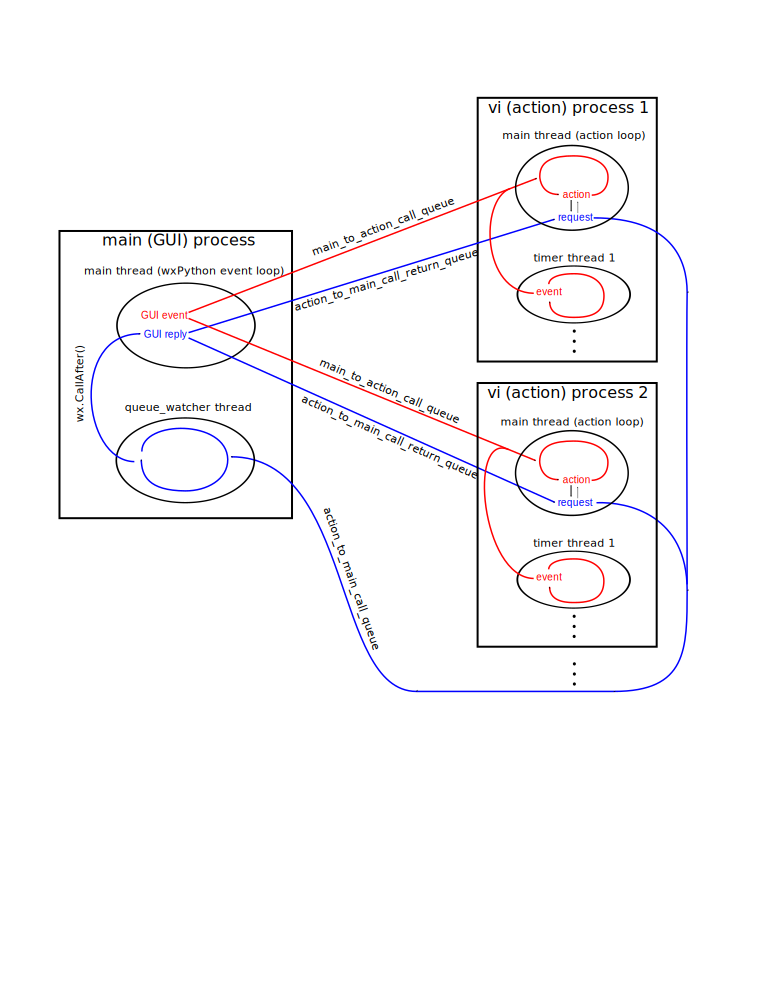
\includegraphics[width=0.800\linewidth]{process_diagram.png}
\caption{Data flow betweeen processes and threads in Pythics.}\end{figure}

Writing code for a new VI in Pythics generally consists of writing two
components:
\begin{enumerate}
\item {} 
A single XML file (a subset of XHTML) to layout the graphical user interface.

\item {} 
One or more text files containing Python code. These give functionality to
the VI.

\end{enumerate}

The XML file is loaded by the GUI process in order to set up the interface,
while the Python code files are loaded and ultimately executed in a VI
subprocess. For each XML file loaded a new tab will be created in the
Pythics window which holds the corresponding VI GUI and a VI subprocess which
handles the associated functionality.

The XML file specifies the layout for the controls in the GUI with a structure
very similar to that used to describe the layout of a web page. Simple tables,
styles, alignments, etc. of text and controls are supported. In the XML file,
parameters may also be passed to controls to setup the behavior of the
controls. The XML file can also direct Pythics to load files which contain
Python code, for example in order to respond to a button press.

The second VI component is one or more text files which contain Python code
and are loaded based on requests in the XML file. The Python code typically
takes the form of a series of Python functions with a particular format. Each
function to be called from the GUI should take an indefinite number of keyword
arguments. In practice, when a GUI control calls a function from one of these
files, Pythics passes the function an object for each control in the GUI with
a \emph{id} attribute. The \emph{id} attribute is used as the name of the
corresponding keyword argument. Additional functions or other code may be
included in the Python code files for use within a VI subprocess. It may sound
complex, but the examples show that this actually a simple and effective
protocol.


\section{XML/HTML File Format}
\label{programming:xml-html-file-format}
The file format which describes the GUI layout in Pythics is an XML-compliant
HTML format, similar to a subset of XHTML. Elements (text, controls, etc.)
within the XML file are controlled by up to three sources within the XML file
in addition to the document structure itself: a cascading style sheet (CSS)
which specifies element \emph{properties} and element \emph{attributes}. The
CSS is located in a \emph{\textless{}style type='text/css'\textgreater{}} element in the document
\emph{\textless{}head\textgreater{}} , and will be described in the section below.

A nearly minimal XML document for Pythics has a \emph{head} with \emph{title} and \emph{style}
elements, and a \emph{body} which contains the controls and other GUI layout
elements:

\begin{Verbatim}[commandchars=\\\{\}]
\textless{}html\textgreater{}

    \textless{}head\textgreater{}

        \textless{}title\textgreater{}Hello World\textless{}/title\textgreater{}

        \textless{}style type='text/css'\textgreater{}

            \textless{}!-- Style Sheet (CSS) goes here --\textgreater{}

        \textless{}/style\textgreater{}

    \textless{}/head\textgreater{}

    \textless{}body\textgreater{}

        \textless{}h1\textgreater{}Hello World\textless{}/h1\textgreater{}

        \textless{}!-- more elements go here for GUI layout --\textgreater{}

    \textless{}/body\textgreater{}

\textless{}/html\textgreater{}
\end{Verbatim}

The \emph{head} is actually completely optional, although the defaults that are used
without a \emph{head} are typically not desirable.


\subsection{HTML Elements}
\label{programming:html-elements}\begin{itemize}
\item {} 
\emph{\textless{}html\textgreater{}}: begin and end \emph{html} tags should surround the whole document

\item {} 
\emph{\textless{}head\textgreater{}}: used to surround the header of the document, which contains \emph{title}
\emph{style} elements

\item {} 
\emph{\textless{}style type='text/css'\textgreater{}}:

\item {} 
\emph{\textless{}title\textgreater{}}: The text between \emph{title} start and end tags will be used as the
VI tab title and the window title when the VI tab is selected

\item {} 
\emph{\textless{}body\textgreater{}}: surrounds the main body of the html document (everything but the
document header)

\item {} 
\emph{\textless{}h1\textgreater{}}, \emph{\textless{}h2\textgreater{}}, ... \emph{\textless{}h6\textgreater{}}: text placed on its own line, typically used for
VI or section names

\item {} 
\emph{\textless{}p\textgreater{}}: text which is not on its own line

\item {} 
\emph{\textless{}hr/\textgreater{}}: insert a horizontal line, typeically as a separator between sections
(no closing tag needed)

\item {} 
\emph{\textless{}br/\textgreater{}}: insert a line break to start the next elements on a new line (no
closing tag needed)

\item {} 
\emph{\textless{}table\textgreater{}}: use a table to arrange elements

\item {} 
\emph{\textless{}object\textgreater{}}: used to insert a control object into a VI interface, see details
below

\end{itemize}


\subsection{Cascading Style Sheets (CSS)}
\label{programming:cascading-style-sheets-css}
A VI's appearance can be specified in a Cascading Style Sheet (CSS), enclosed
between \emph{\textless{}style type='text/css'\textgreater{}} and  \emph{\textless{}/style\textgreater{}} tags within the document
\emph{head}. The style sheet consist of a series of entries separated by white space
(new lines or spaces) of the form:
\emph{selector\{property1:value1; property2:value2\}}
where there may be an arbitrary number of \emph{property:value} pairs separated
by semicolons. The available properties and example values are given below.

The \emph{selector} in a CSS entry may take one of five forms. In order of increasing
specificity, these are:  \emph{tag}, .*class*, \emph{tag}.*class*, \emph{\#id}, and
\emph{tag\#id}. When Pythics encounter an Pythics encounters an XML element in the
body of the document, it searches for a style \emph{property} of a given \emph{element}
as follows, where the first match encountered is used:
\begin{enumerate}
\item {} 
If the element has a \emph{id} attribute: An entry in the style sheet of the form
\emph{tag\#id}, where \emph{tag} is replaced with the element's \emph{tag}, and \emph{id} is
replaced with the element's \emph{id} attribute.

\item {} 
If the element has a \emph{id} attribute: An entry in the style sheet of the form
\emph{\#id}, where \emph{id} is replaced with the element's \emph{id} attribute.

\item {} 
If the element has a \emph{class} attribute: An entry in the style sheet of the
form \emph{tag.class}, where \emph{tag} is replaced with the element's \emph{tag}, and
\emph{class} is replaced with the element's \emph{class} attribute.

\item {} 
If the element has a \emph{class} attribute: An entry in the style sheet of the
form \emph{.class}, where \emph{class} is replaced with the element's \emph{class}
attribute.

\item {} 
An entry matching the element \emph{tag}.

\item {} 
If no entry has been found, the process stated above is repeated for the
parent element containing the original element. As long as no entry is found,
the search keeps proceeding to parent elements until the \emph{body} tag is
reached, which contains a default value for every property.

\end{enumerate}

The following properties can be set in style sheets. Not all properties have
meaning for all element types.

\begin{tabulary}{\linewidth}{|L|L|L|L|}
\hline
\textbf{
Property
} & \textbf{
Description
} & \textbf{
Default
} & \textbf{
Applies to
}\\\hline

\emph{align}
 & 
Alignment of element
 & 
\emph{left}
 & 
all elements
\\\hline

\emph{background-color}
 & 
RGB background color
 & 
\emph{\#eeeeee}
 & 
body only
\\\hline

\emph{margin}
 & 
Margin on left and right side
 & 
\emph{10px}
 & 
body only
\\\hline

\emph{padding}
 & 
Space around element
 & 
\emph{5px}
 & 
all elements
\\\hline

\emph{color}
 & 
Text color
 & 
\emph{black}
 & 
text elements
\\\hline

\emph{font-size}
 & 
Text size
 & 
\emph{12pt}
 & 
text elements
\\\hline

\emph{font-family}
 & 
Family
 & 
\emph{default}
 & 
text elements
\\\hline

\emph{font-style}
 & 
Style
 & 
\emph{normal}
 & 
text elements
\\\hline

\emph{font-weight}
 & 
Weight
 & 
\emph{normal}
 & 
text elements
\\\hline
\end{tabulary}


Here is an example style sheet:

\begin{Verbatim}[commandchars=\\\{\}]
\textless{}style type='text/css'\textgreater{}

body \PYGZob{}background-color: \#eeeeee; margin: 10px; padding: 5px\PYGZcb{}

a \PYGZob{}align: left; color: black; font-size: 8pt; font-family: default; font-style: normal; font-weight: normal\PYGZcb{}

p \PYGZob{}align: left; color: black; font-size: 8pt; font-family: default; font-style: normal; font-weight: normal\PYGZcb{}

h1 \PYGZob{}align: center; font-size: 22pt; font-family: default; font-style: normal; font-weight: bold\PYGZcb{}

h2 \PYGZob{}align: left; font-size: 18pt; font-family: default; font-style: normal; font-weight: normal\PYGZcb{}

h3 \PYGZob{}align: left; font-size: 14pt; font-family: default; font-style: normal; font-weight: normal\PYGZcb{}

h4 \PYGZob{}align: left; font-size: 12pt; font-family: default; font-style: normal; font-weight: normal\PYGZcb{}

h5 \PYGZob{}align: left; font-size: 10pt; font-family: default; font-style: normal; font-weight: normal\PYGZcb{}

h6 \PYGZob{}align: left; font-size: 8pt; font-family: default; font-style: normal; font-weight: normal\PYGZcb{}

object \PYGZob{}align: left\PYGZcb{}

table \PYGZob{}align: center\PYGZcb{}

.cells \PYGZob{}align: left; padding: 1px\PYGZcb{}

.compact \PYGZob{}padding: 0px\PYGZcb{}

\textless{}/style\textgreater{}
\end{Verbatim}


\section{Controls}
\label{programming:controls}
object \emph{parameters} (for controls (\emph{object}) elements only)

A quick example illustrates the differences between object attributes and
parameters:

\begin{Verbatim}[commandchars=\\\{\}]
\textless{}object classid='NumBox' id='voltage' width='200'\textgreater{}
    \textless{}param name='digits' value='3'/\textgreater{}
    \textless{}param name='read\_only' value='True'/\textgreater{}
\textless{}/object\textgreater{}
\end{Verbatim}

In this case, we refer to \emph{id}, \emph{classid}, \emph{width} as \emph{attributes} of \emph{object},
while we refer to \emph{digits} and \emph{read\_only} as \emph{parameters} of \emph{object}, since
they are in \emph{param} elements. Note that \emph{param} elements can only be present
inside of \emph{object} elements.


\subsection{Common Attributes}
\label{programming:common-attributes}
Attributes:
\begin{itemize}
\item {} 
\emph{classid}: A string indicating the type of control to be inserted. For
standard controls, only the name of the control is needed. For custom
controls, it should be of the form `module.class', where \emph{module} is the name
of the module to be imported to find the control class.

\item {} 
\emph{id}: A string used for identifying the control in the html style sheet and
used as the name of the keyword argument when the control is passed to VI
Python code.

\item {} 
\emph{width}: A string giving the width of the control in pixels (default) or in
percent of the window width if the string ends in \emph{\%}.

\item {} 
\emph{height}: A string giving the height of the control in pixels. Many controls
have a reasonable default height so this attribute may not be needed for all
controls.

\end{itemize}


\subsection{Parameters and Python API}
\label{programming:parameters-and-python-api}
See automatically generated API documetation, which lists parameters for
specifying the behavior of each control from the html file as well as the
methods and properties of the control accessible from a VI's Python code.


\chapter{Examples}
\label{examples::doc}\label{examples:examples}\label{examples:id1}
\begin{Verbatim}[commandchars=\\\{\}]
\textless{}html\textgreater{}

\textless{}head\textgreater{}\textless{}title\textgreater{}Hello World\textless{}/title\textgreater{}\textless{}/head\textgreater{}

\textless{}body\textgreater{}



\textless{}h1\textgreater{}Hello World\textless{}/h1\textgreater{}



\textless{}object classid='Button' width='200'\textgreater{}

    \textless{}param name='label' value='Run'/\textgreater{}

    \textless{}param name='action' value='hello\_world.run'/\textgreater{}

\textless{}/object\textgreater{}

\textless{}br/\textgreater{}



\textless{}object classid='TextBox' id='result' width='200'\textgreater{}

\textless{}/object\textgreater{}

\textless{}br/\textgreater{}



\textless{}object classid='ScriptLoader' width='100\%'\textgreater{}

    \textless{}param name='filename' value='hello\_world'/\textgreater{}

\textless{}/object\textgreater{}



\textless{}/body\textgreater{}

\textless{}/html\textgreater{}
\end{Verbatim}

\begin{Verbatim}[commandchars=\\\{\}]
\PYG{k}{def} \PYG{n+nf}{run}\PYG{p}{(}\PYG{n}{result}\PYG{p}{,} \PYG{o}{*}\PYG{o}{*}\PYG{n}{kwargs}\PYG{p}{)}\PYG{p}{:}
    \PYG{n}{result}\PYG{o}{.}\PYG{n}{value} \PYG{o}{=} \PYG{l+s}{"}\PYG{l+s}{Hello, world!}\PYG{l+s}{"}
\end{Verbatim}

See the examples directory of the Pythics distribution for additional examples.


\chapter{Pythics API}
\label{api:pythics-api}\label{api:api}\label{api::doc}
This section describes the html \emph{parameters} as well as the Python attributes
and methods of all the standard controls which are included with the Pythics
distribution.

HTML paramter names and values must always be passed as strings (surrounded
with single or double quotes). Many of the HTML parameter descriptions include
a listing of the allowed values for the parameter, with the default value
emphasized. For example, in (`True' or \emph{`False'}), the value `False' is the
default value if no value is specified.


\section{Controls}
\label{api:controls}
These controls are built in and always loaded. You should omit \code{controls.}
from the start of the \code{classid} when using these controls.
\phantomsection\label{api:module-controls}\index{controls (module)}\index{Button (class in controls)}

\begin{fulllineitems}
\phantomsection\label{api:controls.Button}\pysigline{\strong{class }\code{controls.}\bfcode{Button}}
A push or toggle button which can trigger an action.

HTML Parameters:
\begin{itemize}
\item {} 
\emph{action}: name of a function to run when the button is clicked (\emph{None})

\item {} 
\emph{save}: whether to save the value as a default (\emph{`True'} or `False')

\item {} 
\emph{label}: text to be displayed on the button (\emph{`'})

\item {} 
\emph{toggle}: whether the button should hold the pressed state (`True' or
\emph{`False'})

\end{itemize}
\index{action (controls.Button attribute)}

\begin{fulllineitems}
\phantomsection\label{api:controls.Button.action}\pysigline{\bfcode{action}}
None

\end{fulllineitems}

\index{enabled (controls.Button attribute)}

\begin{fulllineitems}
\phantomsection\label{api:controls.Button.enabled}\pysigline{\bfcode{enabled}}
This property holds whether the control is enabled.

If \emph{enabled} is True, the control handles keyboard and mouse events.
If \emph{enabled} is False, the control does not handle these events and may
be displayed differently.

\end{fulllineitems}

\index{label (controls.Button attribute)}

\begin{fulllineitems}
\phantomsection\label{api:controls.Button.label}\pysigline{\bfcode{label}}
None

\end{fulllineitems}

\index{save (controls.Button attribute)}

\begin{fulllineitems}
\phantomsection\label{api:controls.Button.save}\pysigline{\bfcode{save}}
This property holds whether the control is saved in parameter files.

If \emph{save} is True, the control value is saved.
If \emph{save} is False, the control value is not saved.

\end{fulllineitems}

\index{user (controls.Button attribute)}

\begin{fulllineitems}
\phantomsection\label{api:controls.Button.user}\pysigline{\bfcode{user}}
This property holds arbitrary data that can be set by the user.

The original html parameter value is passes to eval() and stored.

\end{fulllineitems}

\index{value (controls.Button attribute)}

\begin{fulllineitems}
\phantomsection\label{api:controls.Button.value}\pysigline{\bfcode{value}}
None

\end{fulllineitems}


\end{fulllineitems}

\index{CheckBox (class in controls)}

\begin{fulllineitems}
\phantomsection\label{api:controls.CheckBox}\pysigline{\strong{class }\code{controls.}\bfcode{CheckBox}}
A button with a label and a checked or unchecked state.

HTML Parameters:
\begin{itemize}
\item {} 
\emph{action}: name of a function to run when the box is clicked (\emph{None})

\item {} 
\emph{save}: whether to save the value as a default (\emph{`True'} or `False')

\item {} 
\emph{label}: text to display next to the box (\emph{`'})

\end{itemize}
\index{action (controls.CheckBox attribute)}

\begin{fulllineitems}
\phantomsection\label{api:controls.CheckBox.action}\pysigline{\bfcode{action}}
None

\end{fulllineitems}

\index{enabled (controls.CheckBox attribute)}

\begin{fulllineitems}
\phantomsection\label{api:controls.CheckBox.enabled}\pysigline{\bfcode{enabled}}
This property holds whether the control is enabled.

If \emph{enabled} is True, the control handles keyboard and mouse events.
If \emph{enabled} is False, the control does not handle these events and may
be displayed differently.

\end{fulllineitems}

\index{save (controls.CheckBox attribute)}

\begin{fulllineitems}
\phantomsection\label{api:controls.CheckBox.save}\pysigline{\bfcode{save}}
This property holds whether the control is saved in parameter files.

If \emph{save} is True, the control value is saved.
If \emph{save} is False, the control value is not saved.

\end{fulllineitems}

\index{user (controls.CheckBox attribute)}

\begin{fulllineitems}
\phantomsection\label{api:controls.CheckBox.user}\pysigline{\bfcode{user}}
This property holds arbitrary data that can be set by the user.

The original html parameter value is passes to eval() and stored.

\end{fulllineitems}

\index{value (controls.CheckBox attribute)}

\begin{fulllineitems}
\phantomsection\label{api:controls.CheckBox.value}\pysigline{\bfcode{value}}
None

\end{fulllineitems}


\end{fulllineitems}

\index{ChoiceBox (class in controls)}

\begin{fulllineitems}
\phantomsection\label{api:controls.ChoiceBox}\pysigline{\strong{class }\code{controls.}\bfcode{ChoiceBox}}
To be written.

HTML Parameters:
\begin{itemize}
\item {} 
\emph{action}: name of a function to run when a selection is made (\emph{None})

\item {} 
\emph{save}: whether to save the value as a default (\emph{`True'} or `False')

\item {} 
\emph{choices}: (\emph{`{[}{]}'})

\item {} 
\emph{style}: (\emph{`single'}, `multiple', or `extended')

\end{itemize}
\index{action (controls.ChoiceBox attribute)}

\begin{fulllineitems}
\phantomsection\label{api:controls.ChoiceBox.action}\pysigline{\bfcode{action}}
None

\end{fulllineitems}

\index{choices (controls.ChoiceBox attribute)}

\begin{fulllineitems}
\phantomsection\label{api:controls.ChoiceBox.choices}\pysigline{\bfcode{choices}}
None

\end{fulllineitems}

\index{enabled (controls.ChoiceBox attribute)}

\begin{fulllineitems}
\phantomsection\label{api:controls.ChoiceBox.enabled}\pysigline{\bfcode{enabled}}
This property holds whether the control is enabled.

If \emph{enabled} is True, the control handles keyboard and mouse events.
If \emph{enabled} is False, the control does not handle these events and may
be displayed differently.

\end{fulllineitems}

\index{save (controls.ChoiceBox attribute)}

\begin{fulllineitems}
\phantomsection\label{api:controls.ChoiceBox.save}\pysigline{\bfcode{save}}
This property holds whether the control is saved in parameter files.

If \emph{save} is True, the control value is saved.
If \emph{save} is False, the control value is not saved.

\end{fulllineitems}

\index{set\_first\_visible\_item() (controls.ChoiceBox method)}

\begin{fulllineitems}
\phantomsection\label{api:controls.ChoiceBox.set_first_visible_item}\pysiglinewithargsret{\bfcode{set\_first\_visible\_item}}{\emph{value}}{}
None

\end{fulllineitems}

\index{user (controls.ChoiceBox attribute)}

\begin{fulllineitems}
\phantomsection\label{api:controls.ChoiceBox.user}\pysigline{\bfcode{user}}
This property holds arbitrary data that can be set by the user.

The original html parameter value is passes to eval() and stored.

\end{fulllineitems}

\index{value (controls.ChoiceBox attribute)}

\begin{fulllineitems}
\phantomsection\label{api:controls.ChoiceBox.value}\pysigline{\bfcode{value}}
None

\end{fulllineitems}


\end{fulllineitems}

\index{ChoiceButton (class in controls)}

\begin{fulllineitems}
\phantomsection\label{api:controls.ChoiceButton}\pysigline{\strong{class }\code{controls.}\bfcode{ChoiceButton}}
To be written.

HTML Parameters:
\begin{itemize}
\item {} 
\emph{action}: name of a function to run when a selection is made (\emph{None})

\item {} 
\emph{save}: whether to save the value as a default (\emph{`True'} or `False')

\item {} 
\emph{choices}: (\emph{`{[}{]}'})

\end{itemize}
\index{action (controls.ChoiceButton attribute)}

\begin{fulllineitems}
\phantomsection\label{api:controls.ChoiceButton.action}\pysigline{\bfcode{action}}
None

\end{fulllineitems}

\index{choices (controls.ChoiceButton attribute)}

\begin{fulllineitems}
\phantomsection\label{api:controls.ChoiceButton.choices}\pysigline{\bfcode{choices}}
None

\end{fulllineitems}

\index{enabled (controls.ChoiceButton attribute)}

\begin{fulllineitems}
\phantomsection\label{api:controls.ChoiceButton.enabled}\pysigline{\bfcode{enabled}}
This property holds whether the control is enabled.

If \emph{enabled} is True, the control handles keyboard and mouse events.
If \emph{enabled} is False, the control does not handle these events and may
be displayed differently.

\end{fulllineitems}

\index{save (controls.ChoiceButton attribute)}

\begin{fulllineitems}
\phantomsection\label{api:controls.ChoiceButton.save}\pysigline{\bfcode{save}}
This property holds whether the control is saved in parameter files.

If \emph{save} is True, the control value is saved.
If \emph{save} is False, the control value is not saved.

\end{fulllineitems}

\index{user (controls.ChoiceButton attribute)}

\begin{fulllineitems}
\phantomsection\label{api:controls.ChoiceButton.user}\pysigline{\bfcode{user}}
This property holds arbitrary data that can be set by the user.

The original html parameter value is passes to eval() and stored.

\end{fulllineitems}

\index{value (controls.ChoiceButton attribute)}

\begin{fulllineitems}
\phantomsection\label{api:controls.ChoiceButton.value}\pysigline{\bfcode{value}}
None

\end{fulllineitems}


\end{fulllineitems}

\index{EventButton (class in controls)}

\begin{fulllineitems}
\phantomsection\label{api:controls.EventButton}\pysigline{\strong{class }\code{controls.}\bfcode{EventButton}}~\index{action (controls.EventButton attribute)}

\begin{fulllineitems}
\phantomsection\label{api:controls.EventButton.action}\pysigline{\bfcode{action}}
None

\end{fulllineitems}

\index{clear() (controls.EventButton method)}

\begin{fulllineitems}
\phantomsection\label{api:controls.EventButton.clear}\pysiglinewithargsret{\bfcode{clear}}{}{}
\end{fulllineitems}

\index{enabled (controls.EventButton attribute)}

\begin{fulllineitems}
\phantomsection\label{api:controls.EventButton.enabled}\pysigline{\bfcode{enabled}}
This property holds whether the control is enabled.

If \emph{enabled} is True, the control handles keyboard and mouse events.
If \emph{enabled} is False, the control does not handle these events and may
be displayed differently.

\end{fulllineitems}

\index{is\_set() (controls.EventButton method)}

\begin{fulllineitems}
\phantomsection\label{api:controls.EventButton.is_set}\pysiglinewithargsret{\bfcode{is\_set}}{}{}
\end{fulllineitems}

\index{label (controls.EventButton attribute)}

\begin{fulllineitems}
\phantomsection\label{api:controls.EventButton.label}\pysigline{\bfcode{label}}
None

\end{fulllineitems}

\index{save (controls.EventButton attribute)}

\begin{fulllineitems}
\phantomsection\label{api:controls.EventButton.save}\pysigline{\bfcode{save}}
This property holds whether the control is saved in parameter files.

If \emph{save} is True, the control value is saved.
If \emph{save} is False, the control value is not saved.

\end{fulllineitems}

\index{user (controls.EventButton attribute)}

\begin{fulllineitems}
\phantomsection\label{api:controls.EventButton.user}\pysigline{\bfcode{user}}
This property holds arbitrary data that can be set by the user.

The original html parameter value is passes to eval() and stored.

\end{fulllineitems}

\index{value (controls.EventButton attribute)}

\begin{fulllineitems}
\phantomsection\label{api:controls.EventButton.value}\pysigline{\bfcode{value}}
None

\end{fulllineitems}

\index{wait() (controls.EventButton method)}

\begin{fulllineitems}
\phantomsection\label{api:controls.EventButton.wait}\pysiglinewithargsret{\bfcode{wait}}{\emph{t}}{}
\end{fulllineitems}

\index{wait\_interval() (controls.EventButton method)}

\begin{fulllineitems}
\phantomsection\label{api:controls.EventButton.wait_interval}\pysiglinewithargsret{\bfcode{wait\_interval}}{\emph{t}}{}
\end{fulllineitems}


\end{fulllineitems}

\index{FileDialog (class in controls)}

\begin{fulllineitems}
\phantomsection\label{api:controls.FileDialog}\pysigline{\strong{class }\code{controls.}\bfcode{FileDialog}}
To be written.

HTML Parameters:
\begin{itemize}
\item {} 
\emph{title}: (\emph{`Choose a File'})

\item {} 
\emph{directory}: (\emph{`'})

\item {} 
\emph{filter}: (\emph{`*.*'})

\item {} 
\emph{label}: text to show in GUI, set to `' for none (default `FileDialog: id')

\end{itemize}
\index{enabled (controls.FileDialog attribute)}

\begin{fulllineitems}
\phantomsection\label{api:controls.FileDialog.enabled}\pysigline{\bfcode{enabled}}
This property holds whether the control is enabled.

If \emph{enabled} is True, the control handles keyboard and mouse events.
If \emph{enabled} is False, the control does not handle these events and may
be displayed differently.

\end{fulllineitems}

\index{get\_directory() (controls.FileDialog method)}

\begin{fulllineitems}
\phantomsection\label{api:controls.FileDialog.get_directory}\pysiglinewithargsret{\bfcode{get\_directory}}{}{}
None

\end{fulllineitems}

\index{get\_open() (controls.FileDialog method)}

\begin{fulllineitems}
\phantomsection\label{api:controls.FileDialog.get_open}\pysiglinewithargsret{\bfcode{get\_open}}{}{}
None

\end{fulllineitems}

\index{get\_save() (controls.FileDialog method)}

\begin{fulllineitems}
\phantomsection\label{api:controls.FileDialog.get_save}\pysiglinewithargsret{\bfcode{get\_save}}{}{}
None

\end{fulllineitems}

\index{save (controls.FileDialog attribute)}

\begin{fulllineitems}
\phantomsection\label{api:controls.FileDialog.save}\pysigline{\bfcode{save}}
This property holds whether the control is saved in parameter files.

If \emph{save} is True, the control value is saved.
If \emph{save} is False, the control value is not saved.

\end{fulllineitems}

\index{user (controls.FileDialog attribute)}

\begin{fulllineitems}
\phantomsection\label{api:controls.FileDialog.user}\pysigline{\bfcode{user}}
This property holds arbitrary data that can be set by the user.

The original html parameter value is passes to eval() and stored.

\end{fulllineitems}


\end{fulllineitems}

\index{FilePicker (class in controls)}

\begin{fulllineitems}
\phantomsection\label{api:controls.FilePicker}\pysigline{\strong{class }\code{controls.}\bfcode{FilePicker}}
To be written.

HTML Parameters:
\begin{itemize}
\item {} 
\emph{action}: name of a function to run when a file is selected (\emph{None})

\item {} 
\emph{save}: whether to save the value as a default (\emph{`True'} or `False')

\item {} 
\emph{label}: (\emph{`File'})

\item {} 
\emph{title}: (\emph{`Choose'})

\item {} 
\emph{directory}: (\emph{`'})

\item {} 
\emph{filter}: (\emph{`*.*'})

\item {} 
\emph{type}: (`open', \emph{`save'}, or `directory')

\end{itemize}
\index{action (controls.FilePicker attribute)}

\begin{fulllineitems}
\phantomsection\label{api:controls.FilePicker.action}\pysigline{\bfcode{action}}
None

\end{fulllineitems}

\index{browse() (controls.FilePicker method)}

\begin{fulllineitems}
\phantomsection\label{api:controls.FilePicker.browse}\pysiglinewithargsret{\bfcode{browse}}{\emph{*args}, \emph{**kwargs}}{}
None

\end{fulllineitems}

\index{enabled (controls.FilePicker attribute)}

\begin{fulllineitems}
\phantomsection\label{api:controls.FilePicker.enabled}\pysigline{\bfcode{enabled}}
This property holds whether the control is enabled.

If \emph{enabled} is True, the control handles keyboard and mouse events.
If \emph{enabled} is False, the control does not handle these events and may
be displayed differently.

\end{fulllineitems}

\index{save (controls.FilePicker attribute)}

\begin{fulllineitems}
\phantomsection\label{api:controls.FilePicker.save}\pysigline{\bfcode{save}}
This property holds whether the control is saved in parameter files.

If \emph{save} is True, the control value is saved.
If \emph{save} is False, the control value is not saved.

\end{fulllineitems}

\index{user (controls.FilePicker attribute)}

\begin{fulllineitems}
\phantomsection\label{api:controls.FilePicker.user}\pysigline{\bfcode{user}}
This property holds arbitrary data that can be set by the user.

The original html parameter value is passes to eval() and stored.

\end{fulllineitems}

\index{value (controls.FilePicker attribute)}

\begin{fulllineitems}
\phantomsection\label{api:controls.FilePicker.value}\pysigline{\bfcode{value}}
None

\end{fulllineitems}


\end{fulllineitems}

\index{GlobalAction (class in controls)}

\begin{fulllineitems}
\phantomsection\label{api:controls.GlobalAction}\pysigline{\strong{class }\code{controls.}\bfcode{GlobalAction}}
Holds an action which can triggered by a \emph{GlobalTrigger} control in another VI.

The \emph{id} parameter is the name of the control and it must match the
`action\_id' of an associated \emph{GlobalTrigger}. The GlobalAction and
GlobalTrigger may be in different vi's.

HTML Parameters:
\begin{itemize}
\item {} 
\emph{action}: name of a function to run when the control is triggered (default None)

\item {} 
\emph{label}: text to show in GUI, set to `' for none (default `GlobalAction: id')

\end{itemize}
\index{action (controls.GlobalAction attribute)}

\begin{fulllineitems}
\phantomsection\label{api:controls.GlobalAction.action}\pysigline{\bfcode{action}}
Name of a function to run when the control is triggered.

\end{fulllineitems}

\index{enabled (controls.GlobalAction attribute)}

\begin{fulllineitems}
\phantomsection\label{api:controls.GlobalAction.enabled}\pysigline{\bfcode{enabled}}
This property holds whether the control is enabled.

If \emph{enabled} is True, the control handles keyboard and mouse events.
If \emph{enabled} is False, the control does not handle these events and may
be displayed differently.

\end{fulllineitems}

\index{save (controls.GlobalAction attribute)}

\begin{fulllineitems}
\phantomsection\label{api:controls.GlobalAction.save}\pysigline{\bfcode{save}}
This property holds whether the control is saved in parameter files.

If \emph{save} is True, the control value is saved.
If \emph{save} is False, the control value is not saved.

\end{fulllineitems}

\index{user (controls.GlobalAction attribute)}

\begin{fulllineitems}
\phantomsection\label{api:controls.GlobalAction.user}\pysigline{\bfcode{user}}
This property holds arbitrary data that can be set by the user.

The original html parameter value is passes to eval() and stored.

\end{fulllineitems}


\end{fulllineitems}

\index{GlobalNamespace (class in controls)}

\begin{fulllineitems}
\phantomsection\label{api:controls.GlobalNamespace}\pysigline{\strong{class }\code{controls.}\bfcode{GlobalNamespace}}
Creates a namespace that is shared between all VIs. GlobalNamespaces in
different vi's with the same \emph{id} attribute will share the same namespace.

HTML Parameters:
\begin{itemize}
\item {} 
\emph{label}: text to show in GUI, set to `' for none (default `GlobalNamespace: id')

\end{itemize}
\index{enabled (controls.GlobalNamespace attribute)}

\begin{fulllineitems}
\phantomsection\label{api:controls.GlobalNamespace.enabled}\pysigline{\bfcode{enabled}}
This property holds whether the control is enabled.

If \emph{enabled} is True, the control handles keyboard and mouse events.
If \emph{enabled} is False, the control does not handle these events and may
be displayed differently.

\end{fulllineitems}

\index{save (controls.GlobalNamespace attribute)}

\begin{fulllineitems}
\phantomsection\label{api:controls.GlobalNamespace.save}\pysigline{\bfcode{save}}
This property holds whether the control is saved in parameter files.

If \emph{save} is True, the control value is saved.
If \emph{save} is False, the control value is not saved.

\end{fulllineitems}

\index{user (controls.GlobalNamespace attribute)}

\begin{fulllineitems}
\phantomsection\label{api:controls.GlobalNamespace.user}\pysigline{\bfcode{user}}
This property holds arbitrary data that can be set by the user.

The original html parameter value is passes to eval() and stored.

\end{fulllineitems}


\end{fulllineitems}

\index{GlobalTrigger (class in controls)}

\begin{fulllineitems}
\phantomsection\label{api:controls.GlobalTrigger}\pysigline{\strong{class }\code{controls.}\bfcode{GlobalTrigger}}
A control to trigger any \emph{GlobalAction} with an \emph{id} that matches the
`action\_id' paramter.

The GlobalAction and GlobalTrigger may be in different vi's.

HTML Parameters:
\begin{itemize}
\item {} 
\emph{action\_id}: text to match to a `GlobalAction' id

\item {} 
\emph{label}: text to show in GUI, set to `' for none (default `GlobalTrigger:  id: action\_id')

\end{itemize}
\index{enabled (controls.GlobalTrigger attribute)}

\begin{fulllineitems}
\phantomsection\label{api:controls.GlobalTrigger.enabled}\pysigline{\bfcode{enabled}}
This property holds whether the control is enabled.

If \emph{enabled} is True, the control handles keyboard and mouse events.
If \emph{enabled} is False, the control does not handle these events and may
be displayed differently.

\end{fulllineitems}

\index{save (controls.GlobalTrigger attribute)}

\begin{fulllineitems}
\phantomsection\label{api:controls.GlobalTrigger.save}\pysigline{\bfcode{save}}
This property holds whether the control is saved in parameter files.

If \emph{save} is True, the control value is saved.
If \emph{save} is False, the control value is not saved.

\end{fulllineitems}

\index{trigger() (controls.GlobalTrigger method)}

\begin{fulllineitems}
\phantomsection\label{api:controls.GlobalTrigger.trigger}\pysiglinewithargsret{\bfcode{trigger}}{}{}
Trigger all GlobalActions with a matching \emph{key}.

\end{fulllineitems}

\index{user (controls.GlobalTrigger attribute)}

\begin{fulllineitems}
\phantomsection\label{api:controls.GlobalTrigger.user}\pysigline{\bfcode{user}}
This property holds arbitrary data that can be set by the user.

The original html parameter value is passes to eval() and stored.

\end{fulllineitems}


\end{fulllineitems}

\index{Image (class in controls)}

\begin{fulllineitems}
\phantomsection\label{api:controls.Image}\pysigline{\strong{class }\code{controls.}\bfcode{Image}}
To be written.

HTML Parameters:
\begin{itemize}
\item {} 
\emph{action}: name of a function to run when the box is clicked (\emph{None})

\item {} 
\emph{save}: whether to save the value as a default (\emph{`True'} or `False')

\item {} 
\emph{fit}: (`True' or \emph{`False'})

\item {} 
\emph{scale}: (\emph{`1.0'})

\item {} 
\emph{use\_shared\_memory}: (`True' or \emph{`False'})

\item {} 
\emph{image\_dimensions}: (\emph{None})

\item {} 
\emph{left\_press\_action}: (\emph{None})

\item {} 
\emph{right\_press\_action}: (\emph{None})

\item {} 
\emph{left\_release\_action}: (\emph{None})

\item {} 
\emph{right\_release\_action}: (\emph{None})

\item {} 
\emph{left\_double\_click\_action}: (\emph{None})

\item {} 
\emph{right\_double\_click\_action}: (\emph{None})

\end{itemize}
\index{enabled (controls.Image attribute)}

\begin{fulllineitems}
\phantomsection\label{api:controls.Image.enabled}\pysigline{\bfcode{enabled}}
This property holds whether the control is enabled.

If \emph{enabled} is True, the control handles keyboard and mouse events.
If \emph{enabled} is False, the control does not handle these events and may
be displayed differently.

\end{fulllineitems}

\index{image (controls.Image attribute)}

\begin{fulllineitems}
\phantomsection\label{api:controls.Image.image}\pysigline{\bfcode{image}}
None

\end{fulllineitems}

\index{image\_with\_shared (controls.Image attribute)}

\begin{fulllineitems}
\phantomsection\label{api:controls.Image.image_with_shared}\pysigline{\bfcode{image\_with\_shared}}
None

\end{fulllineitems}

\index{left\_double\_click\_action (controls.Image attribute)}

\begin{fulllineitems}
\phantomsection\label{api:controls.Image.left_double_click_action}\pysigline{\bfcode{left\_double\_click\_action}}
None

\end{fulllineitems}

\index{left\_double\_click\_position (controls.Image attribute)}

\begin{fulllineitems}
\phantomsection\label{api:controls.Image.left_double_click_position}\pysigline{\bfcode{left\_double\_click\_position}}
None

\end{fulllineitems}

\index{left\_press\_action (controls.Image attribute)}

\begin{fulllineitems}
\phantomsection\label{api:controls.Image.left_press_action}\pysigline{\bfcode{left\_press\_action}}
None

\end{fulllineitems}

\index{left\_press\_position (controls.Image attribute)}

\begin{fulllineitems}
\phantomsection\label{api:controls.Image.left_press_position}\pysigline{\bfcode{left\_press\_position}}
None

\end{fulllineitems}

\index{left\_release\_action (controls.Image attribute)}

\begin{fulllineitems}
\phantomsection\label{api:controls.Image.left_release_action}\pysigline{\bfcode{left\_release\_action}}
None

\end{fulllineitems}

\index{left\_release\_position (controls.Image attribute)}

\begin{fulllineitems}
\phantomsection\label{api:controls.Image.left_release_position}\pysigline{\bfcode{left\_release\_position}}
None

\end{fulllineitems}

\index{right\_double\_click\_action (controls.Image attribute)}

\begin{fulllineitems}
\phantomsection\label{api:controls.Image.right_double_click_action}\pysigline{\bfcode{right\_double\_click\_action}}
None

\end{fulllineitems}

\index{right\_double\_click\_position (controls.Image attribute)}

\begin{fulllineitems}
\phantomsection\label{api:controls.Image.right_double_click_position}\pysigline{\bfcode{right\_double\_click\_position}}
None

\end{fulllineitems}

\index{right\_press\_action (controls.Image attribute)}

\begin{fulllineitems}
\phantomsection\label{api:controls.Image.right_press_action}\pysigline{\bfcode{right\_press\_action}}
None

\end{fulllineitems}

\index{right\_press\_position (controls.Image attribute)}

\begin{fulllineitems}
\phantomsection\label{api:controls.Image.right_press_position}\pysigline{\bfcode{right\_press\_position}}
None

\end{fulllineitems}

\index{right\_release\_action (controls.Image attribute)}

\begin{fulllineitems}
\phantomsection\label{api:controls.Image.right_release_action}\pysigline{\bfcode{right\_release\_action}}
None

\end{fulllineitems}

\index{right\_release\_position (controls.Image attribute)}

\begin{fulllineitems}
\phantomsection\label{api:controls.Image.right_release_position}\pysigline{\bfcode{right\_release\_position}}
None

\end{fulllineitems}

\index{save (controls.Image attribute)}

\begin{fulllineitems}
\phantomsection\label{api:controls.Image.save}\pysigline{\bfcode{save}}
This property holds whether the control is saved in parameter files.

If \emph{save} is True, the control value is saved.
If \emph{save} is False, the control value is not saved.

\end{fulllineitems}

\index{user (controls.Image attribute)}

\begin{fulllineitems}
\phantomsection\label{api:controls.Image.user}\pysigline{\bfcode{user}}
This property holds arbitrary data that can be set by the user.

The original html parameter value is passes to eval() and stored.

\end{fulllineitems}


\end{fulllineitems}

\index{ImageButton (class in controls)}

\begin{fulllineitems}
\phantomsection\label{api:controls.ImageButton}\pysigline{\strong{class }\code{controls.}\bfcode{ImageButton}}
To be written.

HTML Parameters:
\begin{itemize}
\item {} 
\emph{action}: name of a function to run when the box is clicked (\emph{None})

\item {} 
\emph{save}: whether to save the value as a default (\emph{`True'} or `False')

\item {} 
\emph{toggle}: (`True' or \emph{`False'})

\item {} 
\emph{image\_filename}: (\emph{None})

\item {} 
\emph{pressed\_image\_filename}: (\emph{None})

\end{itemize}
\index{action (controls.ImageButton attribute)}

\begin{fulllineitems}
\phantomsection\label{api:controls.ImageButton.action}\pysigline{\bfcode{action}}
None

\end{fulllineitems}

\index{enabled (controls.ImageButton attribute)}

\begin{fulllineitems}
\phantomsection\label{api:controls.ImageButton.enabled}\pysigline{\bfcode{enabled}}
This property holds whether the control is enabled.

If \emph{enabled} is True, the control handles keyboard and mouse events.
If \emph{enabled} is False, the control does not handle these events and may
be displayed differently.

\end{fulllineitems}

\index{save (controls.ImageButton attribute)}

\begin{fulllineitems}
\phantomsection\label{api:controls.ImageButton.save}\pysigline{\bfcode{save}}
This property holds whether the control is saved in parameter files.

If \emph{save} is True, the control value is saved.
If \emph{save} is False, the control value is not saved.

\end{fulllineitems}

\index{user (controls.ImageButton attribute)}

\begin{fulllineitems}
\phantomsection\label{api:controls.ImageButton.user}\pysigline{\bfcode{user}}
This property holds arbitrary data that can be set by the user.

The original html parameter value is passes to eval() and stored.

\end{fulllineitems}

\index{value (controls.ImageButton attribute)}

\begin{fulllineitems}
\phantomsection\label{api:controls.ImageButton.value}\pysigline{\bfcode{value}}
None

\end{fulllineitems}


\end{fulllineitems}

\index{MessageDialog (class in controls)}

\begin{fulllineitems}
\phantomsection\label{api:controls.MessageDialog}\pysigline{\strong{class }\code{controls.}\bfcode{MessageDialog}}
To be written.

HTML Parameters:
\begin{itemize}
\item {} 
\emph{title}: (\emph{`MessageDialog'})

\item {} 
\emph{message}: (\emph{`'})

\item {} 
\emph{ok\_button}: (`True' or \emph{`False'})

\item {} 
\emph{cancel\_button}: (`True' or \emph{`False'})

\item {} 
\emph{yes\_button}: (`True' or \emph{`False'})

\item {} 
\emph{no\_button}: (`True' or \emph{`False'})

\item {} 
\emph{abort\_button}: (`True' or \emph{`False'})

\item {} 
\emph{retry\_button}: (`True' or \emph{`False'})

\item {} 
\emph{ignore\_button}: (`True' or \emph{`False'})

\item {} 
\emph{severity}: (\emph{`None'}, `question', `information', `warning', or `critical')

\item {} 
\emph{label}: text to show in GUI, set to `' for none (default `MessageDialog: id')

\end{itemize}
\index{enabled (controls.MessageDialog attribute)}

\begin{fulllineitems}
\phantomsection\label{api:controls.MessageDialog.enabled}\pysigline{\bfcode{enabled}}
This property holds whether the control is enabled.

If \emph{enabled} is True, the control handles keyboard and mouse events.
If \emph{enabled} is False, the control does not handle these events and may
be displayed differently.

\end{fulllineitems}

\index{message (controls.MessageDialog attribute)}

\begin{fulllineitems}
\phantomsection\label{api:controls.MessageDialog.message}\pysigline{\bfcode{message}}
None

\end{fulllineitems}

\index{open() (controls.MessageDialog method)}

\begin{fulllineitems}
\phantomsection\label{api:controls.MessageDialog.open}\pysiglinewithargsret{\bfcode{open}}{}{}
None

\end{fulllineitems}

\index{save (controls.MessageDialog attribute)}

\begin{fulllineitems}
\phantomsection\label{api:controls.MessageDialog.save}\pysigline{\bfcode{save}}
This property holds whether the control is saved in parameter files.

If \emph{save} is True, the control value is saved.
If \emph{save} is False, the control value is not saved.

\end{fulllineitems}

\index{severity (controls.MessageDialog attribute)}

\begin{fulllineitems}
\phantomsection\label{api:controls.MessageDialog.severity}\pysigline{\bfcode{severity}}
None

\end{fulllineitems}

\index{user (controls.MessageDialog attribute)}

\begin{fulllineitems}
\phantomsection\label{api:controls.MessageDialog.user}\pysigline{\bfcode{user}}
This property holds arbitrary data that can be set by the user.

The original html parameter value is passes to eval() and stored.

\end{fulllineitems}


\end{fulllineitems}

\index{NumBox (class in controls)}

\begin{fulllineitems}
\phantomsection\label{api:controls.NumBox}\pysigline{\strong{class }\code{controls.}\bfcode{NumBox}}
To be written.

HTML Parameters:
\begin{itemize}
\item {} 
\emph{action}: name of a function to run when the value is changeed (\emph{None})

\item {} 
\emph{save}: whether to save the value as a default (\emph{`True'} or `False')

\item {} 
\emph{read\_only}: (`True' or \emph{`False'})

\item {} 
\emph{align}: (\emph{`left'}, `center' or `right')

\item {} 
\emph{increment}: (\emph{`1'})

\item {} 
\emph{digits}: number of digits to show after the decimal point (\emph{`1'})

\item {} \begin{description}
\item[{\emph{notation}: how to enter and display numbers. `scientific' enables }] \leavevmode
scientific notation and formats the number according to `format\_str'
(\emph{`decimal'} or `scientific')

\end{description}

\item {} \begin{description}
\item[{\emph{format\_str}: printf style format string used to format number if }] \leavevmode
`notation' is `scientific' (\emph{`\%g'})

\end{description}

\item {} 
\emph{maximum}: (\emph{None})

\item {} 
\emph{minimum}: (\emph{None})

\item {} 
\emph{prefix}: text to show before the value, e.g. `\$' (\emph{`'})

\item {} 
\emph{suffix}: text to shwo after the value, e.g. a unit (\emph{`'})

\end{itemize}
\index{action (controls.NumBox attribute)}

\begin{fulllineitems}
\phantomsection\label{api:controls.NumBox.action}\pysigline{\bfcode{action}}
None

\end{fulllineitems}

\index{enabled (controls.NumBox attribute)}

\begin{fulllineitems}
\phantomsection\label{api:controls.NumBox.enabled}\pysigline{\bfcode{enabled}}
This property holds whether the control is enabled.

If \emph{enabled} is True, the control handles keyboard and mouse events.
If \emph{enabled} is False, the control does not handle these events and may
be displayed differently.

\end{fulllineitems}

\index{save (controls.NumBox attribute)}

\begin{fulllineitems}
\phantomsection\label{api:controls.NumBox.save}\pysigline{\bfcode{save}}
This property holds whether the control is saved in parameter files.

If \emph{save} is True, the control value is saved.
If \emph{save} is False, the control value is not saved.

\end{fulllineitems}

\index{user (controls.NumBox attribute)}

\begin{fulllineitems}
\phantomsection\label{api:controls.NumBox.user}\pysigline{\bfcode{user}}
This property holds arbitrary data that can be set by the user.

The original html parameter value is passes to eval() and stored.

\end{fulllineitems}

\index{value (controls.NumBox attribute)}

\begin{fulllineitems}
\phantomsection\label{api:controls.NumBox.value}\pysigline{\bfcode{value}}
None

\end{fulllineitems}


\end{fulllineitems}

\index{ParameterLoader (class in controls)}

\begin{fulllineitems}
\phantomsection\label{api:controls.ParameterLoader}\pysigline{\strong{class }\code{controls.}\bfcode{ParameterLoader}}
Loads VI parameters from a file and sets that file as the default.

HTML Parameters:
\begin{itemize}
\item {} 
\emph{filename}: name of the file to load the parameters from

\item {} 
\emph{label}: text to show in GUI, set to `' for none (default `ParameterLoader: filename')

\end{itemize}
\index{enabled (controls.ParameterLoader attribute)}

\begin{fulllineitems}
\phantomsection\label{api:controls.ParameterLoader.enabled}\pysigline{\bfcode{enabled}}
This property holds whether the control is enabled.

If \emph{enabled} is True, the control handles keyboard and mouse events.
If \emph{enabled} is False, the control does not handle these events and may
be displayed differently.

\end{fulllineitems}

\index{save (controls.ParameterLoader attribute)}

\begin{fulllineitems}
\phantomsection\label{api:controls.ParameterLoader.save}\pysigline{\bfcode{save}}
This property holds whether the control is saved in parameter files.

If \emph{save} is True, the control value is saved.
If \emph{save} is False, the control value is not saved.

\end{fulllineitems}

\index{user (controls.ParameterLoader attribute)}

\begin{fulllineitems}
\phantomsection\label{api:controls.ParameterLoader.user}\pysigline{\bfcode{user}}
This property holds arbitrary data that can be set by the user.

The original html parameter value is passes to eval() and stored.

\end{fulllineitems}


\end{fulllineitems}

\index{Plot2D (class in controls)}

\begin{fulllineitems}
\phantomsection\label{api:controls.Plot2D}\pysigline{\strong{class }\code{controls.}\bfcode{Plot2D}}
An easy to use plotting control for 2-dimensional plotting.
Right click on the plot to save an image of the plot to a file.

HTML parameters (values must be given in quotation marks):
\begin{quote}
\begin{description}
\item[{\emph{projection}: {[} `cartesian' (default) \textbar{} `polar' {]}}] \leavevmode
Set to polar for polar plots (not all plot items supported).

\end{description}
\end{quote}
\index{append\_data() (controls.Plot2D method)}

\begin{fulllineitems}
\phantomsection\label{api:controls.Plot2D.append_data}\pysiglinewithargsret{\bfcode{append\_data}}{\emph{key}, \emph{data}, \emph{redraw=True}, \emph{rescale='auto'}}{}
Append data to a plot item.

Only works with curves which were created with 
\emph{memory} = `circular' or \emph{memory} = `growable'.

Arguments:
\begin{quote}
\begin{description}
\item[{\emph{key}: str}] \leavevmode
The name you gave to the plot item when it was created.

\item[{\emph{data}: one or two-dimensional numpy array, list, or tuple}] \leavevmode
The new data to be appended to the previous data of the plot item.
\emph{data} should be a single point of the form (x, y) or a series of
points of the form ((x1, y1), (x2, y2), ...).

\end{description}
\end{quote}

Keyword arguments:
\begin{quote}
\begin{description}
\item[{\emph{redraw}: {[} \emph{True}  (default) \textbar{} \emph{False} {]}}] \leavevmode
Whether to redraw the plot after applying changes.

\item[{\emph{rescale}: {[} `auto' (default) \textbar{} \emph{True} \textbar{} \emph{False} {]}}] \leavevmode
Whether to rescale the plot. If `auto', then only rescale if needed.

\end{description}
\end{quote}

\end{fulllineitems}

\index{axes\_enter\_action (controls.Plot2D attribute)}

\begin{fulllineitems}
\phantomsection\label{api:controls.Plot2D.axes_enter_action}\pysigline{\bfcode{axes\_enter\_action}}
None

\end{fulllineitems}

\index{axes\_leave\_action (controls.Plot2D attribute)}

\begin{fulllineitems}
\phantomsection\label{api:controls.Plot2D.axes_leave_action}\pysigline{\bfcode{axes\_leave\_action}}
None

\end{fulllineitems}

\index{button\_press\_action (controls.Plot2D attribute)}

\begin{fulllineitems}
\phantomsection\label{api:controls.Plot2D.button_press_action}\pysigline{\bfcode{button\_press\_action}}
None

\end{fulllineitems}

\index{button\_release\_action (controls.Plot2D attribute)}

\begin{fulllineitems}
\phantomsection\label{api:controls.Plot2D.button_release_action}\pysigline{\bfcode{button\_release\_action}}
None

\end{fulllineitems}

\index{clear() (controls.Plot2D method)}

\begin{fulllineitems}
\phantomsection\label{api:controls.Plot2D.clear}\pysiglinewithargsret{\bfcode{clear}}{\emph{redraw=True}, \emph{rescale='auto'}}{}
Delete all plot items to clear the plot.

Optional keyword arguments:
\begin{quote}
\begin{description}
\item[{\emph{redraw}: {[} \emph{True}  (default) \textbar{} \emph{False} {]}}] \leavevmode
Whether to redraw the plot after applying changes.

\item[{\emph{rescale}: {[} `auto' (default) \textbar{} \emph{True} \textbar{} \emph{False} {]}}] \leavevmode
Whether to rescale the plot. If `auto', then only rescale if needed.

\end{description}
\end{quote}

\end{fulllineitems}

\index{clear\_data() (controls.Plot2D method)}

\begin{fulllineitems}
\phantomsection\label{api:controls.Plot2D.clear_data}\pysiglinewithargsret{\bfcode{clear\_data}}{\emph{key}, \emph{redraw=True}, \emph{rescale='auto'}}{}
Delete all the data of a plot item.

Arguments:
\begin{quote}
\begin{description}
\item[{\emph{key}: str}] \leavevmode
The name you gave to the plot item when it was created.

\end{description}
\end{quote}

Optional keyword arguments:
\begin{quote}
\begin{description}
\item[{\emph{redraw}: {[} \emph{True}  (default) \textbar{} \emph{False} {]}}] \leavevmode
Whether to redraw the plot after applying changes.

\item[{\emph{rescale}: {[} `auto' (default) \textbar{} \emph{True} \textbar{} \emph{False} {]}}] \leavevmode
Whether to rescale the plot. If `auto', then only rescale if needed.

\end{description}
\end{quote}

\end{fulllineitems}

\index{clear\_events() (controls.Plot2D method)}

\begin{fulllineitems}
\phantomsection\label{api:controls.Plot2D.clear_events}\pysiglinewithargsret{\bfcode{clear\_events}}{}{}
None

\end{fulllineitems}

\index{delete() (controls.Plot2D method)}

\begin{fulllineitems}
\phantomsection\label{api:controls.Plot2D.delete}\pysiglinewithargsret{\bfcode{delete}}{\emph{key}, \emph{redraw=True}, \emph{rescale='auto'}}{}
Delete a plot item.

Arguments:
\begin{quote}
\begin{description}
\item[{\emph{key}: str}] \leavevmode
The name you gave to the plot item when it was created.

\end{description}
\end{quote}

Optional keyword arguments:
\begin{quote}
\begin{description}
\item[{\emph{redraw}: {[} \emph{True}  (default) \textbar{} \emph{False} {]}}] \leavevmode
Whether to redraw the plot after applying changes.

\item[{\emph{rescale}: {[} `auto' (default) \textbar{} \emph{True} \textbar{} \emph{False} {]}}] \leavevmode
Whether to rescale the plot. If `auto', then only rescale if needed.

\end{description}
\end{quote}

\end{fulllineitems}

\index{draw\_action (controls.Plot2D attribute)}

\begin{fulllineitems}
\phantomsection\label{api:controls.Plot2D.draw_action}\pysigline{\bfcode{draw\_action}}
None

\end{fulllineitems}

\index{enabled (controls.Plot2D attribute)}

\begin{fulllineitems}
\phantomsection\label{api:controls.Plot2D.enabled}\pysigline{\bfcode{enabled}}
This property holds whether the control is enabled.

If \emph{enabled} is True, the control handles keyboard and mouse events.
If \emph{enabled} is False, the control does not handle these events and may
be displayed differently.

\end{fulllineitems}

\index{events\_length (controls.Plot2D attribute)}

\begin{fulllineitems}
\phantomsection\label{api:controls.Plot2D.events_length}\pysigline{\bfcode{events\_length}}
None

\end{fulllineitems}

\index{figure\_enter\_action (controls.Plot2D attribute)}

\begin{fulllineitems}
\phantomsection\label{api:controls.Plot2D.figure_enter_action}\pysigline{\bfcode{figure\_enter\_action}}
None

\end{fulllineitems}

\index{figure\_leave\_action (controls.Plot2D attribute)}

\begin{fulllineitems}
\phantomsection\label{api:controls.Plot2D.figure_leave_action}\pysigline{\bfcode{figure\_leave\_action}}
None

\end{fulllineitems}

\index{key\_press\_action (controls.Plot2D attribute)}

\begin{fulllineitems}
\phantomsection\label{api:controls.Plot2D.key_press_action}\pysigline{\bfcode{key\_press\_action}}
None

\end{fulllineitems}

\index{key\_release\_action (controls.Plot2D attribute)}

\begin{fulllineitems}
\phantomsection\label{api:controls.Plot2D.key_release_action}\pysigline{\bfcode{key\_release\_action}}
None

\end{fulllineitems}

\index{motion\_notify\_action (controls.Plot2D attribute)}

\begin{fulllineitems}
\phantomsection\label{api:controls.Plot2D.motion_notify_action}\pysigline{\bfcode{motion\_notify\_action}}
None

\end{fulllineitems}

\index{new\_colormesh() (controls.Plot2D method)}

\begin{fulllineitems}
\phantomsection\label{api:controls.Plot2D.new_colormesh}\pysiglinewithargsret{\bfcode{new\_colormesh}}{\emph{key}, \emph{X}, \emph{Y}, \emph{**kwargs}}{}
Create a new pseudocolor mesh item on the plot.

Arguments:
\begin{quote}
\begin{description}
\item[{\emph{key}: str}] \leavevmode
The name you give to this plot item for future access.

\item[{\emph{X}: str}] \leavevmode
The x coordinates of the colored quadrilaterals.
\emph{numpy.meshgrid()} may be helpful for making this.

\item[{\emph{Y}: str}] \leavevmode
The x coordinates of the colored quadrilaterals.
\emph{numpy.meshgrid()} may be helpful for making this.

\end{description}
\end{quote}

Optional keyword arguments:
\begin{quote}
\begin{description}
\item[{\emph{animated}: {[} \emph{True} \textbar{} \emph{False} (default) {]}}] \leavevmode
If \emph{True}, try to redraw this item without redrawing the whole plot
whenever it is updated. This is generally faster if the axes do not
need to be rescaled, and thus is recommended for plot items that 
are changed frequently.

\item[{\emph{alpha}: \code{0 \textless{}= scalar \textless{}= 1}}] \leavevmode
The alpha value for the image. 0.0 is transparent and 1.0 is opaque.

\item[{\emph{extent}:  {[} \emph{None} (default) \textbar{} scalars (left, right, bottom, top) {]}}] \leavevmode
Data limits for the axes. The default assigns zero-based row, 
column indices to the x, y centers of the pixels.

\item[{\emph{interpolation}: str}] \leavevmode
Acceptable values are `none', `nearest', `bilinear',
`bicubic', `spline16', `spline36', `hanning', `hamming',
`hermite', `kaiser', `quadric', `catrom', `gaussian',
`bessel', `mitchell', `sinc', `lanczos'

\item[{\emph{colormap}: str}] \leavevmode
The name of a matplotlib colormap for mapping the data value to the
displayed color at each point.

\emph{colormap} is ignored when \emph{data} has RGB(A) information

\item[{\emph{c\_limits}:  {[} `auto' (default) \textbar{} scalars (vmin, vmax) {]}}] \leavevmode
Data limits for the colormap.

\end{description}
\end{quote}

\end{fulllineitems}

\index{new\_curve() (controls.Plot2D method)}

\begin{fulllineitems}
\phantomsection\label{api:controls.Plot2D.new_curve}\pysiglinewithargsret{\bfcode{new\_curve}}{\emph{key}, \emph{memory='array'}, \emph{length=1000}, \emph{**kwargs}}{}
Create a new curve or set of points on the plot.

Arguments:
\begin{quote}
\begin{description}
\item[{\emph{key}: str}] \leavevmode
The name you give to this plot item for future access.

\end{description}
\end{quote}

Optional keyword arguments:
\begin{quote}
\begin{description}
\item[{\emph{memory}: {[} `array' (default) \textbar{} `circular' \textbar{} `growable' {]}}] \leavevmode
Format for plot item data storage which determines how future updates 
to the data can be made.

\item[{\emph{length}: int}] \leavevmode
if \emph{memory} == `circular': The number of elements in the circular array.
if \emph{memory} == `growable': The initial number of elements in the array.

\item[{\emph{animated}: {[} \emph{True} \textbar{} \emph{False} (default) {]}}] \leavevmode
If \emph{True}, try to redraw this item without redrawing the whole plot
whenever it is updated. This is generally faster if the axes do not
need to be rescaled, and thus is recommended for plot items that 
are changed frequently.

\item[{\emph{alpha}: \code{0 \textless{}= scalar \textless{}= 1}}] \leavevmode
The alpha value for the curve. 0.0 is transparent and 1.0 is opaque.

\item[{\emph{line\_color}: any valid color, see more information below}] \leavevmode
The color used for drawing lines between points.

\end{description}

\emph{line\_style}: {[} `-` \textbar{} `--` \textbar{} `-.' \textbar{} `:' \textbar{} `' {]}
\begin{quote}

The following format string characters are accepted to control
the line style:

\begin{tabulary}{\linewidth}{|L|L|}
\hline
\textbf{
character
} & \textbf{
description
}\\\hline

\code{'-'}
 & 
solid line style (default)
\\\hline

\code{'-{-}'}
 & 
dashed line style
\\\hline

\code{'-.'}
 & 
dash-dot line style
\\\hline

\code{':'}
 & 
dotted line style
\\\hline

\code{''}
 & 
no line
\\\hline
\end{tabulary}

\end{quote}
\begin{description}
\item[{\emph{line\_width}: float value in points}] \leavevmode
The width of lines between points.

\item[{\emph{marker\_color}: any valid color, see more information below}] \leavevmode
The fill color of markers drawn at the specified points.

\item[{\emph{marker\_edge\_color}: any valid color, see more information below}] \leavevmode
The color of the edges of markers or of the whole marker if the
marker consists of lines only.

\item[{\emph{marker\_edge\_width}: float value in points}] \leavevmode
The width of the edges of markers or of the lines if the marker 
consists of lines only.

\item[{\emph{marker\_style}: any valid marker style, see table below}] \leavevmode
The shape of the markers drawn.

The following format string characters are accepted to control
the marker style:

\begin{tabulary}{\linewidth}{|L|L|}
\hline
\textbf{
Value
} & \textbf{
Description
}\\\hline

\code{''}
 & 
no marker (default)
\\\hline

\code{'.'}
 & 
point marker
\\\hline

\code{','}
 & 
pixel marker
\\\hline

\code{'o'}
 & 
circle marker
\\\hline

\code{'v'}
 & 
triangle\_down marker
\\\hline

\code{'\textasciicircum{}'}
 & 
triangle\_up marker
\\\hline

\code{'\textless{}'}
 & 
triangle\_left marker
\\\hline

\code{'\textgreater{}'}
 & 
triangle\_right marker
\\\hline

\code{'1'}
 & 
tri\_down marker
\\\hline

\code{'2'}
 & 
tri\_up marker
\\\hline

\code{'3'}
 & 
tri\_left marker
\\\hline

\code{'4'}
 & 
tri\_right marker
\\\hline

\code{'s'}
 & 
square marker
\\\hline

\code{'p'}
 & 
pentagon marker
\\\hline

\code{'*'}
 & 
star marker
\\\hline

\code{'h'}
 & 
hexagon1 marker
\\\hline

\code{'H'}
 & 
hexagon2 marker
\\\hline

\code{'+'}
 & 
plus marker
\\\hline

\code{'x'}
 & 
x marker
\\\hline

\code{'D'}
 & 
diamond marker
\\\hline

\code{'d'}
 & 
thin\_diamond marker
\\\hline

\code{'\textbar{}'}
 & 
vline marker
\\\hline

\code{'\_'}
 & 
hline marker
\\\hline

(\emph{numsides}, \emph{style}, \emph{angle})
 & 
see below
\\\hline
\end{tabulary}


The marker can also be a tuple (\emph{numsides}, \emph{style}, \emph{angle}), 
which will create a custom, regular symbol.
\begin{quote}
\begin{description}
\item[{\emph{numsides}:}] \leavevmode
the number of sides

\item[{\emph{style}:}] \leavevmode
the style of the regular symbol:

\begin{tabulary}{\linewidth}{|L|L|}
\hline
\textbf{
Value
} & \textbf{
Description
}\\\hline

0
 & 
a regular polygon
\\\hline

1
 & 
a star-like symbol
\\\hline

2
 & 
an asterisk
\\\hline

3
 & 
a circle (\emph{numsides} and \emph{angle} is ignored)
\\\hline
\end{tabulary}


\item[{\emph{angle}:}] \leavevmode
the angle of rotation of the symbol

\end{description}
\end{quote}

\item[{\emph{marker\_width}: float value in points}] \leavevmode
The overall size of the markers draw at the data points.

\end{description}
\end{quote}

Colors:
\begin{quote}

The following color abbreviations are supported:
\begin{quote}

\begin{tabulary}{\linewidth}{|L|L|}
\hline
\textbf{
Value
} & \textbf{
Color
}\\\hline

`b'
 & 
blue
\\\hline

`g'
 & 
green
\\\hline

`r'
 & 
red
\\\hline

`c'
 & 
cyan
\\\hline

`m'
 & 
magenta
\\\hline

`y'
 & 
yellow
\\\hline

`k'
 & 
black
\\\hline

`w'
 & 
white
\\\hline
\end{tabulary}

\end{quote}
\end{quote}

In addition, you can specify colors in many other ways, including 
full names (\code{'green'}), hex strings (\code{'\#008000'}), RGB or 
RGBA tuples (\code{(0,1,0,1)}) or grayscale intensities as a string (\code{'0.8'}).

\end{fulllineitems}

\index{new\_image() (controls.Plot2D method)}

\begin{fulllineitems}
\phantomsection\label{api:controls.Plot2D.new_image}\pysiglinewithargsret{\bfcode{new\_image}}{\emph{key}, \emph{**kwargs}}{}
Create a new image item on the plot.

Arguments:
\begin{quote}
\begin{description}
\item[{\emph{key}: str}] \leavevmode
The name you give to this plot item for future access.

\end{description}
\end{quote}

Optional keyword arguments:
\begin{quote}
\begin{description}
\item[{\emph{animated}: {[} \emph{True} \textbar{} \emph{False} (default) {]}}] \leavevmode
If \emph{True}, try to redraw this item without redrawing the whole plot
whenever it is updated. This is generally faster if the axes do not
need to be rescaled, and thus is recommended for plot items that 
are changed frequently.

\item[{\emph{alpha}: \code{0 \textless{}= scalar \textless{}= 1}}] \leavevmode
The alpha value for the image. 0.0 is transparent and 1.0 is opaque.

\item[{\emph{extent}:  {[} \emph{None} (default) \textbar{} scalars (left, right, bottom, top) {]}}] \leavevmode
Data limits for the axes. The default assigns zero-based row, 
column indices to the x, y centers of the pixels.

\item[{\emph{interpolation}: str}] \leavevmode
Acceptable values are `none', `nearest', `bilinear',
`bicubic', `spline16', `spline36', `hanning', `hamming',
`hermite', `kaiser', `quadric', `catrom', `gaussian',
`bessel', `mitchell', `sinc', `lanczos'

\item[{\emph{origin}: {[} None \textbar{} `upper' \textbar{} `lower' {]}}] \leavevmode
Place the {[}0,0{]} index of the array in the upper left or lower left 
corner of the axes.

\item[{\emph{colormap}: str}] \leavevmode
The name of a matplotlib colormap for mapping the data value to the
displayed color at each point.

\emph{colormap} is ignored when \emph{data} has RGB(A) information

\item[{\emph{c\_limits}:  {[} `auto' (default) \textbar{} scalars (vmin, vmax) {]}}] \leavevmode
Data limits for the colormap.

\end{description}
\end{quote}

\end{fulllineitems}

\index{pick\_action (controls.Plot2D attribute)}

\begin{fulllineitems}
\phantomsection\label{api:controls.Plot2D.pick_action}\pysigline{\bfcode{pick\_action}}
None

\end{fulllineitems}

\index{pop\_event() (controls.Plot2D method)}

\begin{fulllineitems}
\phantomsection\label{api:controls.Plot2D.pop_event}\pysiglinewithargsret{\bfcode{pop\_event}}{}{}
None

\end{fulllineitems}

\index{resize\_action (controls.Plot2D attribute)}

\begin{fulllineitems}
\phantomsection\label{api:controls.Plot2D.resize_action}\pysigline{\bfcode{resize\_action}}
None

\end{fulllineitems}

\index{save (controls.Plot2D attribute)}

\begin{fulllineitems}
\phantomsection\label{api:controls.Plot2D.save}\pysigline{\bfcode{save}}
This property holds whether the control is saved in parameter files.

If \emph{save} is True, the control value is saved.
If \emph{save} is False, the control value is not saved.

\end{fulllineitems}

\index{save\_figure() (controls.Plot2D method)}

\begin{fulllineitems}
\phantomsection\label{api:controls.Plot2D.save_figure}\pysiglinewithargsret{\bfcode{save\_figure}}{\emph{filename=None}, \emph{rescale='auto'}}{}
Save an image of the plot to a file.

Optional keyword arguments:
\begin{quote}
\begin{description}
\item[{\emph{filename}: str}] \leavevmode
The name of the file to save to. If no filename is given, a dialog
box in which to choose a filname will be presented.

\item[{\emph{rescale}: {[} `auto' (default) \textbar{} \emph{True} \textbar{} \emph{False} {]}}] \leavevmode
Whether to rescale the plot. If `auto', then only rescale if needed.

\end{description}
\end{quote}

\end{fulllineitems}

\index{scroll\_action (controls.Plot2D attribute)}

\begin{fulllineitems}
\phantomsection\label{api:controls.Plot2D.scroll_action}\pysigline{\bfcode{scroll\_action}}
None

\end{fulllineitems}

\index{set\_data() (controls.Plot2D method)}

\begin{fulllineitems}
\phantomsection\label{api:controls.Plot2D.set_data}\pysiglinewithargsret{\bfcode{set\_data}}{\emph{key}, \emph{data}, \emph{redraw=True}, \emph{rescale='auto'}}{}
Change the data of a plot item.

Arguments:
\begin{quote}
\begin{description}
\item[{\emph{key}: str}] \leavevmode
The name you gave to the plot item when it was created.

\item[{\emph{data}: two-dimensional numpy array, list, or tuple or a PIL image}] \leavevmode
The new data to be assigned to the plot item.

For curves, \emph{data} should be a series of points 
of the form ((x1, y1), (x2, y2), ...).

For images, \emph{data} should be a two dimensional float array, a uint8 
array or a PIL image. If \emph{data} is an array, \emph{data} can have the 
following shapes:
\begin{itemize}
\item {} 
MxN -- luminance (grayscale, float array only)

\item {} 
MxNx3 -- RGB (float or uint8 array)

\item {} 
MxNx4 -- RGBA (float or uint8 array)

\end{itemize}

The value for each component of MxNx3 and MxNx4 float arrays should be
in the range 0.0 to 1.0; MxN float arrays may be normalized.

For colormeshes, \emph{data} is a 2-D array, and the dimensions of \emph{X} 
and \emph{Y} should be one greater than those of \emph{data}.

\end{description}
\end{quote}

Optional keyword arguments:
\begin{quote}
\begin{description}
\item[{\emph{redraw}: {[} \emph{True}  (default) \textbar{} \emph{False} {]}}] \leavevmode
Whether to redraw the plot after applying changes.

\item[{\emph{rescale}: {[} `auto' (default) \textbar{} \emph{True} \textbar{} \emph{False} {]}}] \leavevmode
Whether to rescale the plot. If `auto', then only rescale if needed.

\end{description}
\end{quote}

\end{fulllineitems}

\index{set\_plot\_properties() (controls.Plot2D method)}

\begin{fulllineitems}
\phantomsection\label{api:controls.Plot2D.set_plot_properties}\pysiglinewithargsret{\bfcode{set\_plot\_properties}}{\emph{redraw=True}, \emph{rescale='auto'}, \emph{**kwargs}}{}
Set the graphical properties of a plot.

Optional keyword arguments:
\begin{quote}

\emph{aspect\_ratio}: {[}'auto' (default) \textbar{} `equal' \textbar{} a number {]}

\emph{x\_limits}: {[}'auto' (default) \textbar{} scalars (x\_min, x\_max){]}

\emph{y\_limits}: {[}'auto' (default) \textbar{} scalars (y\_min, y\_max){]}

\emph{tight\_autoscale}: {[}\emph{True} \textbar{} \emph{False} (default){]}
\begin{description}
\item[{\emph{x\_scale}: {[}'linear' (default) \textbar{} `log'{]}}] \leavevmode
Scaling of the x-axis.

\item[{\emph{y\_scale}: {[}'linear' (default) \textbar{} `log'{]}}] \leavevmode
Scaling of the y-axis.

\item[{\emph{title}: str}] \leavevmode
Title to be drawn above the plot.

\item[{\emph{x\_label}: str}] \leavevmode
Label to be drawn on the x-axis of the plot.

\item[{\emph{y\_label}: str}] \leavevmode
Label to be drawn on the y-axis of the plot.

\item[{\emph{dpi}: int}] \leavevmode
Resolution (dots per inch) of plots saved to files.

\item[{\emph{redraw}: {[} \emph{True}  (default) \textbar{} \emph{False} {]}}] \leavevmode
Whether to redraw the plot after applying changes.

\item[{\emph{rescale}: {[} `auto' (default) \textbar{} \emph{True} \textbar{} \emph{False} {]}}] \leavevmode
Whether to rescale the plot. If `auto', then only rescale if needed.

\end{description}
\end{quote}

\end{fulllineitems}

\index{set\_properties() (controls.Plot2D method)}

\begin{fulllineitems}
\phantomsection\label{api:controls.Plot2D.set_properties}\pysiglinewithargsret{\bfcode{set\_properties}}{\emph{key}, \emph{redraw=True}, \emph{rescale='auto'}, \emph{**kwargs}}{}
Set the graphical properties of a plot item.

Arguments:
\begin{quote}
\begin{description}
\item[{\emph{key}: str}] \leavevmode
The name you gave to the plot item when it was created.

\end{description}
\end{quote}

Optional keyword arguments:
\begin{quote}

Any of the the keyword arguments describing the graphical representation 
of the plot item that can be given when the item is created.
\begin{description}
\item[{\emph{redraw}: {[} \emph{True}  (default) \textbar{} \emph{False} {]}}] \leavevmode
Whether to redraw the plot after applying changes.

\item[{\emph{rescale}: {[} `auto' (default) \textbar{} \emph{True} \textbar{} \emph{False} {]}}] \leavevmode
Whether to rescale the plot. If `auto', then only rescale if needed.

\end{description}
\end{quote}

\end{fulllineitems}

\index{user (controls.Plot2D attribute)}

\begin{fulllineitems}
\phantomsection\label{api:controls.Plot2D.user}\pysigline{\bfcode{user}}
This property holds arbitrary data that can be set by the user.

The original html parameter value is passes to eval() and stored.

\end{fulllineitems}


\end{fulllineitems}

\index{RadioButtonBox (class in controls)}

\begin{fulllineitems}
\phantomsection\label{api:controls.RadioButtonBox}\pysigline{\strong{class }\code{controls.}\bfcode{RadioButtonBox}}
To be written.

HTML Parameters:
\begin{itemize}
\item {} 
\emph{action}: name of a function to run when a button is clicked (\emph{None})

\item {} 
\emph{save}: whether to save the value as a default (\emph{`True'} or `False')

\item {} 
\emph{label}: (\emph{`'})

\item {} 
\emph{rows}: (\emph{None})

\item {} 
\emph{columns}: (\emph{None})

\item {} 
\emph{choices}: (\emph{`{[}{]}'})

\end{itemize}
\index{action (controls.RadioButtonBox attribute)}

\begin{fulllineitems}
\phantomsection\label{api:controls.RadioButtonBox.action}\pysigline{\bfcode{action}}
None

\end{fulllineitems}

\index{enabled (controls.RadioButtonBox attribute)}

\begin{fulllineitems}
\phantomsection\label{api:controls.RadioButtonBox.enabled}\pysigline{\bfcode{enabled}}
This property holds whether the control is enabled.

If \emph{enabled} is True, the control handles keyboard and mouse events.
If \emph{enabled} is False, the control does not handle these events and may
be displayed differently.

\end{fulllineitems}

\index{save (controls.RadioButtonBox attribute)}

\begin{fulllineitems}
\phantomsection\label{api:controls.RadioButtonBox.save}\pysigline{\bfcode{save}}
This property holds whether the control is saved in parameter files.

If \emph{save} is True, the control value is saved.
If \emph{save} is False, the control value is not saved.

\end{fulllineitems}

\index{user (controls.RadioButtonBox attribute)}

\begin{fulllineitems}
\phantomsection\label{api:controls.RadioButtonBox.user}\pysigline{\bfcode{user}}
This property holds arbitrary data that can be set by the user.

The original html parameter value is passes to eval() and stored.

\end{fulllineitems}

\index{value (controls.RadioButtonBox attribute)}

\begin{fulllineitems}
\phantomsection\label{api:controls.RadioButtonBox.value}\pysigline{\bfcode{value}}
None

\end{fulllineitems}


\end{fulllineitems}

\index{ScriptLoader (class in controls)}

\begin{fulllineitems}
\phantomsection\label{api:controls.ScriptLoader}\pysigline{\strong{class }\code{controls.}\bfcode{ScriptLoader}}
Imports a Python file for use by the VI process.

HTML Parameters:
\begin{itemize}
\item {} 
\emph{filename}: name of the python file to import with no extension

\item {} 
\emph{initialization\_action}: name of a function to run after the VI is loaded (default None)

\item {} 
\emph{termination\_action}: name of a function to run before the VI is terminated (default None)

\item {} 
\emph{label}: text to show in GUI, set to `' for none (default `ScriptLoader: filename')

\end{itemize}
\index{enabled (controls.ScriptLoader attribute)}

\begin{fulllineitems}
\phantomsection\label{api:controls.ScriptLoader.enabled}\pysigline{\bfcode{enabled}}
This property holds whether the control is enabled.

If \emph{enabled} is True, the control handles keyboard and mouse events.
If \emph{enabled} is False, the control does not handle these events and may
be displayed differently.

\end{fulllineitems}

\index{save (controls.ScriptLoader attribute)}

\begin{fulllineitems}
\phantomsection\label{api:controls.ScriptLoader.save}\pysigline{\bfcode{save}}
This property holds whether the control is saved in parameter files.

If \emph{save} is True, the control value is saved.
If \emph{save} is False, the control value is not saved.

\end{fulllineitems}

\index{user (controls.ScriptLoader attribute)}

\begin{fulllineitems}
\phantomsection\label{api:controls.ScriptLoader.user}\pysigline{\bfcode{user}}
This property holds arbitrary data that can be set by the user.

The original html parameter value is passes to eval() and stored.

\end{fulllineitems}


\end{fulllineitems}

\index{ScrollBar (class in controls)}

\begin{fulllineitems}
\phantomsection\label{api:controls.ScrollBar}\pysigline{\strong{class }\code{controls.}\bfcode{ScrollBar}}
To be written.

HTML Parameters:
\begin{itemize}
\item {} 
\emph{action}: name of a function to run when the box is clicked (\emph{None})

\item {} 
\emph{save}: whether to save the value as a default (\emph{`True'} or `False')

\item {} 
\emph{tracking}: (`True' or  \emph{`False'})

\item {} 
\emph{orientation}: (\emph{`horizontal'} or `vertical')

\end{itemize}
\index{action (controls.ScrollBar attribute)}

\begin{fulllineitems}
\phantomsection\label{api:controls.ScrollBar.action}\pysigline{\bfcode{action}}
None

\end{fulllineitems}

\index{enabled (controls.ScrollBar attribute)}

\begin{fulllineitems}
\phantomsection\label{api:controls.ScrollBar.enabled}\pysigline{\bfcode{enabled}}
This property holds whether the control is enabled.

If \emph{enabled} is True, the control handles keyboard and mouse events.
If \emph{enabled} is False, the control does not handle these events and may
be displayed differently.

\end{fulllineitems}

\index{ranges (controls.ScrollBar attribute)}

\begin{fulllineitems}
\phantomsection\label{api:controls.ScrollBar.ranges}\pysigline{\bfcode{ranges}}
None

\end{fulllineitems}

\index{save (controls.ScrollBar attribute)}

\begin{fulllineitems}
\phantomsection\label{api:controls.ScrollBar.save}\pysigline{\bfcode{save}}
This property holds whether the control is saved in parameter files.

If \emph{save} is True, the control value is saved.
If \emph{save} is False, the control value is not saved.

\end{fulllineitems}

\index{user (controls.ScrollBar attribute)}

\begin{fulllineitems}
\phantomsection\label{api:controls.ScrollBar.user}\pysigline{\bfcode{user}}
This property holds arbitrary data that can be set by the user.

The original html parameter value is passes to eval() and stored.

\end{fulllineitems}

\index{value (controls.ScrollBar attribute)}

\begin{fulllineitems}
\phantomsection\label{api:controls.ScrollBar.value}\pysigline{\bfcode{value}}
None

\end{fulllineitems}


\end{fulllineitems}

\index{Shell (class in controls)}

\begin{fulllineitems}
\phantomsection\label{api:controls.Shell}\pysigline{\strong{class }\code{controls.}\bfcode{Shell}}~\index{enabled (controls.Shell attribute)}

\begin{fulllineitems}
\phantomsection\label{api:controls.Shell.enabled}\pysigline{\bfcode{enabled}}
This property holds whether the control is enabled.

If \emph{enabled} is True, the control handles keyboard and mouse events.
If \emph{enabled} is False, the control does not handle these events and may
be displayed differently.

\end{fulllineitems}

\index{interact() (controls.Shell method)}

\begin{fulllineitems}
\phantomsection\label{api:controls.Shell.interact}\pysiglinewithargsret{\bfcode{interact}}{\emph{local\_dict}, \emph{banner=None}}{}
\end{fulllineitems}

\index{message() (controls.Shell method)}

\begin{fulllineitems}
\phantomsection\label{api:controls.Shell.message}\pysiglinewithargsret{\bfcode{message}}{\emph{message}}{}
None

\end{fulllineitems}

\index{push() (controls.Shell method)}

\begin{fulllineitems}
\phantomsection\label{api:controls.Shell.push}\pysiglinewithargsret{\bfcode{push}}{\emph{line}}{}
\end{fulllineitems}

\index{resetbuffer() (controls.Shell method)}

\begin{fulllineitems}
\phantomsection\label{api:controls.Shell.resetbuffer}\pysiglinewithargsret{\bfcode{resetbuffer}}{}{}
\end{fulllineitems}

\index{save (controls.Shell attribute)}

\begin{fulllineitems}
\phantomsection\label{api:controls.Shell.save}\pysigline{\bfcode{save}}
This property holds whether the control is saved in parameter files.

If \emph{save} is True, the control value is saved.
If \emph{save} is False, the control value is not saved.

\end{fulllineitems}

\index{user (controls.Shell attribute)}

\begin{fulllineitems}
\phantomsection\label{api:controls.Shell.user}\pysigline{\bfcode{user}}
This property holds arbitrary data that can be set by the user.

The original html parameter value is passes to eval() and stored.

\end{fulllineitems}

\index{write() (controls.Shell method)}

\begin{fulllineitems}
\phantomsection\label{api:controls.Shell.write}\pysiglinewithargsret{\bfcode{write}}{\emph{text}}{}
None

\end{fulllineitems}


\end{fulllineitems}

\index{SubWindow (class in controls)}

\begin{fulllineitems}
\phantomsection\label{api:controls.SubWindow}\pysigline{\strong{class }\code{controls.}\bfcode{SubWindow}}
To be written.

HTML Parameters:
\begin{itemize}
\item {} 
\emph{filename}: (\emph{`'})

\end{itemize}
\index{enabled (controls.SubWindow attribute)}

\begin{fulllineitems}
\phantomsection\label{api:controls.SubWindow.enabled}\pysigline{\bfcode{enabled}}
This property holds whether the control is enabled.

If \emph{enabled} is True, the control handles keyboard and mouse events.
If \emph{enabled} is False, the control does not handle these events and may
be displayed differently.

\end{fulllineitems}

\index{save (controls.SubWindow attribute)}

\begin{fulllineitems}
\phantomsection\label{api:controls.SubWindow.save}\pysigline{\bfcode{save}}
This property holds whether the control is saved in parameter files.

If \emph{save} is True, the control value is saved.
If \emph{save} is False, the control value is not saved.

\end{fulllineitems}

\index{user (controls.SubWindow attribute)}

\begin{fulllineitems}
\phantomsection\label{api:controls.SubWindow.user}\pysigline{\bfcode{user}}
This property holds arbitrary data that can be set by the user.

The original html parameter value is passes to eval() and stored.

\end{fulllineitems}


\end{fulllineitems}

\index{TextBox (class in controls)}

\begin{fulllineitems}
\phantomsection\label{api:controls.TextBox}\pysigline{\strong{class }\code{controls.}\bfcode{TextBox}}
To be written.

HTML Parameters:
\begin{itemize}
\item {} 
\emph{action}: name of a function to run when the value is changed (\emph{None})

\item {} 
\emph{save}: whether to save the value as a default (\emph{`True'} or `False')

\item {} 
\emph{align}: (\emph{`left'}, `center' or `right')

\item {} 
\emph{multiline}: (`True' or \emph{`False'})

\item {} 
\emph{read\_only}: (`True' or \emph{`False'})

\item {} 
\emph{font}: name of font to use for shell text (\emph{Consolas})

\item {} 
\emph{font\_size}: size of font to use for shell text in points (\emph{10})

\end{itemize}
\index{action (controls.TextBox attribute)}

\begin{fulllineitems}
\phantomsection\label{api:controls.TextBox.action}\pysigline{\bfcode{action}}
None

\end{fulllineitems}

\index{enabled (controls.TextBox attribute)}

\begin{fulllineitems}
\phantomsection\label{api:controls.TextBox.enabled}\pysigline{\bfcode{enabled}}
This property holds whether the control is enabled.

If \emph{enabled} is True, the control handles keyboard and mouse events.
If \emph{enabled} is False, the control does not handle these events and may
be displayed differently.

\end{fulllineitems}

\index{save (controls.TextBox attribute)}

\begin{fulllineitems}
\phantomsection\label{api:controls.TextBox.save}\pysigline{\bfcode{save}}
This property holds whether the control is saved in parameter files.

If \emph{save} is True, the control value is saved.
If \emph{save} is False, the control value is not saved.

\end{fulllineitems}

\index{scroll() (controls.TextBox method)}

\begin{fulllineitems}
\phantomsection\label{api:controls.TextBox.scroll}\pysiglinewithargsret{\bfcode{scroll}}{\emph{dx}, \emph{dy}}{}
None

\end{fulllineitems}

\index{user (controls.TextBox attribute)}

\begin{fulllineitems}
\phantomsection\label{api:controls.TextBox.user}\pysigline{\bfcode{user}}
This property holds arbitrary data that can be set by the user.

The original html parameter value is passes to eval() and stored.

\end{fulllineitems}

\index{value (controls.TextBox attribute)}

\begin{fulllineitems}
\phantomsection\label{api:controls.TextBox.value}\pysigline{\bfcode{value}}
None

\end{fulllineitems}


\end{fulllineitems}

\index{TextIOBox (class in controls)}

\begin{fulllineitems}
\phantomsection\label{api:controls.TextIOBox}\pysigline{\strong{class }\code{controls.}\bfcode{TextIOBox}}
To be written.

HTML Parameters:
\begin{itemize}
\item {} 
\emph{save}: whether to save the value as a default (`True' or \emph{`False'})

\item {} 
\emph{align}: (\emph{`left'}, `center', or `right')

\item {} 
\emph{auto\_update}: (\emph{`True'} or `False')

\item {} 
\emph{reverse}: (`True' or \emph{`False'})

\item {} 
\emph{font}: name of font to use for shell text (\emph{Consolas})

\item {} 
\emph{font\_size}: size of font to use for shell text in points (\emph{10})

\end{itemize}
\index{action (controls.TextIOBox attribute)}

\begin{fulllineitems}
\phantomsection\label{api:controls.TextIOBox.action}\pysigline{\bfcode{action}}
None

\end{fulllineitems}

\index{clear() (controls.TextIOBox method)}

\begin{fulllineitems}
\phantomsection\label{api:controls.TextIOBox.clear}\pysiglinewithargsret{\bfcode{clear}}{\emph{*args}, \emph{**kwargs}}{}
None

\end{fulllineitems}

\index{close() (controls.TextIOBox method)}

\begin{fulllineitems}
\phantomsection\label{api:controls.TextIOBox.close}\pysiglinewithargsret{\bfcode{close}}{\emph{*args}, \emph{**kwargs}}{}
None

\end{fulllineitems}

\index{enabled (controls.TextIOBox attribute)}

\begin{fulllineitems}
\phantomsection\label{api:controls.TextIOBox.enabled}\pysigline{\bfcode{enabled}}
This property holds whether the control is enabled.

If \emph{enabled} is True, the control handles keyboard and mouse events.
If \emph{enabled} is False, the control does not handle these events and may
be displayed differently.

\end{fulllineitems}

\index{flush() (controls.TextIOBox method)}

\begin{fulllineitems}
\phantomsection\label{api:controls.TextIOBox.flush}\pysiglinewithargsret{\bfcode{flush}}{\emph{*args}, \emph{**kwargs}}{}
None

\end{fulllineitems}

\index{getvalue() (controls.TextIOBox method)}

\begin{fulllineitems}
\phantomsection\label{api:controls.TextIOBox.getvalue}\pysiglinewithargsret{\bfcode{getvalue}}{\emph{*args}, \emph{**kwargs}}{}
None

\end{fulllineitems}

\index{isatty() (controls.TextIOBox method)}

\begin{fulllineitems}
\phantomsection\label{api:controls.TextIOBox.isatty}\pysiglinewithargsret{\bfcode{isatty}}{\emph{*args}, \emph{**kwargs}}{}
None

\end{fulllineitems}

\index{next() (controls.TextIOBox method)}

\begin{fulllineitems}
\phantomsection\label{api:controls.TextIOBox.next}\pysiglinewithargsret{\bfcode{next}}{\emph{*args}, \emph{**kwargs}}{}
None

\end{fulllineitems}

\index{read() (controls.TextIOBox method)}

\begin{fulllineitems}
\phantomsection\label{api:controls.TextIOBox.read}\pysiglinewithargsret{\bfcode{read}}{\emph{*args}, \emph{**kwargs}}{}
None

\end{fulllineitems}

\index{readline() (controls.TextIOBox method)}

\begin{fulllineitems}
\phantomsection\label{api:controls.TextIOBox.readline}\pysiglinewithargsret{\bfcode{readline}}{\emph{*args}, \emph{**kwargs}}{}
None

\end{fulllineitems}

\index{readlines() (controls.TextIOBox method)}

\begin{fulllineitems}
\phantomsection\label{api:controls.TextIOBox.readlines}\pysiglinewithargsret{\bfcode{readlines}}{\emph{*args}, \emph{**kwargs}}{}
None

\end{fulllineitems}

\index{reset() (controls.TextIOBox method)}

\begin{fulllineitems}
\phantomsection\label{api:controls.TextIOBox.reset}\pysiglinewithargsret{\bfcode{reset}}{\emph{*args}, \emph{**kwargs}}{}
None

\end{fulllineitems}

\index{save (controls.TextIOBox attribute)}

\begin{fulllineitems}
\phantomsection\label{api:controls.TextIOBox.save}\pysigline{\bfcode{save}}
This property holds whether the control is saved in parameter files.

If \emph{save} is True, the control value is saved.
If \emph{save} is False, the control value is not saved.

\end{fulllineitems}

\index{scroll() (controls.TextIOBox method)}

\begin{fulllineitems}
\phantomsection\label{api:controls.TextIOBox.scroll}\pysiglinewithargsret{\bfcode{scroll}}{\emph{dx}, \emph{dy}}{}
None

\end{fulllineitems}

\index{seek() (controls.TextIOBox method)}

\begin{fulllineitems}
\phantomsection\label{api:controls.TextIOBox.seek}\pysiglinewithargsret{\bfcode{seek}}{\emph{*args}, \emph{**kwargs}}{}
None

\end{fulllineitems}

\index{tell() (controls.TextIOBox method)}

\begin{fulllineitems}
\phantomsection\label{api:controls.TextIOBox.tell}\pysiglinewithargsret{\bfcode{tell}}{\emph{*args}, \emph{**kwargs}}{}
None

\end{fulllineitems}

\index{truncate() (controls.TextIOBox method)}

\begin{fulllineitems}
\phantomsection\label{api:controls.TextIOBox.truncate}\pysiglinewithargsret{\bfcode{truncate}}{\emph{*args}, \emph{**kwargs}}{}
None

\end{fulllineitems}

\index{user (controls.TextIOBox attribute)}

\begin{fulllineitems}
\phantomsection\label{api:controls.TextIOBox.user}\pysigline{\bfcode{user}}
This property holds arbitrary data that can be set by the user.

The original html parameter value is passes to eval() and stored.

\end{fulllineitems}

\index{value (controls.TextIOBox attribute)}

\begin{fulllineitems}
\phantomsection\label{api:controls.TextIOBox.value}\pysigline{\bfcode{value}}
None

\end{fulllineitems}

\index{write() (controls.TextIOBox method)}

\begin{fulllineitems}
\phantomsection\label{api:controls.TextIOBox.write}\pysiglinewithargsret{\bfcode{write}}{\emph{*args}, \emph{**kwargs}}{}
None

\end{fulllineitems}

\index{writelines() (controls.TextIOBox method)}

\begin{fulllineitems}
\phantomsection\label{api:controls.TextIOBox.writelines}\pysiglinewithargsret{\bfcode{writelines}}{\emph{*args}, \emph{**kwargs}}{}
None

\end{fulllineitems}


\end{fulllineitems}

\index{Timer (class in controls)}

\begin{fulllineitems}
\phantomsection\label{api:controls.Timer}\pysigline{\strong{class }\code{controls.}\bfcode{Timer}}
A control which makes calls to \emph{action} at regular time intervals. Most 
settings are controlled in a call to \emph{start}, which begins the timer. The 
timer can be stopped by calling the \emph{stop} method. The timer may be started 
and stopped multiple times. Due to the mult-threaded nature of Timers, most
control properties are read-only and can only be set by calling \emph{start}.

HTML Parameters:
\begin{itemize}
\item {} 
\emph{action}: name of a function to run when the timer is triggered (\emph{None})

\item {} 
\emph{label}: text to show in GUI, set to `' for none (default `Timer: id')

\end{itemize}
\index{action (controls.Timer attribute)}

\begin{fulllineitems}
\phantomsection\label{api:controls.Timer.action}\pysigline{\bfcode{action}}
\end{fulllineitems}

\index{interval (controls.Timer attribute)}

\begin{fulllineitems}
\phantomsection\label{api:controls.Timer.interval}\pysigline{\bfcode{interval}}
\end{fulllineitems}

\index{retrigger() (controls.Timer method)}

\begin{fulllineitems}
\phantomsection\label{api:controls.Timer.retrigger}\pysiglinewithargsret{\bfcode{retrigger}}{}{}
\end{fulllineitems}

\index{running (controls.Timer attribute)}

\begin{fulllineitems}
\phantomsection\label{api:controls.Timer.running}\pysigline{\bfcode{running}}
\end{fulllineitems}

\index{start() (controls.Timer method)}

\begin{fulllineitems}
\phantomsection\label{api:controls.Timer.start}\pysiglinewithargsret{\bfcode{start}}{\emph{interval=1.0}, \emph{action=None}, \emph{call\_at\_zero=True}, \emph{require\_retrigger=False}, \emph{retrigger\_timeout=None}}{}
\end{fulllineitems}

\index{stop() (controls.Timer method)}

\begin{fulllineitems}
\phantomsection\label{api:controls.Timer.stop}\pysiglinewithargsret{\bfcode{stop}}{}{}
\end{fulllineitems}


\end{fulllineitems}



\section{Matplotlib Controls}
\label{api:matplotlib-controls}
These controls are from the matplotlib library. This library optional for
Pythics (although strongly recommended for plotting) and is not loaded if none
of these controls are used. When these controls are used, the \code{classid} must
begin with \code{mpl.}.
\phantomsection\label{api:module-mpl}\index{mpl (module)}\index{Canvas (class in mpl)}

\begin{fulllineitems}
\phantomsection\label{api:mpl.Canvas}\pysigline{\strong{class }\code{mpl.}\bfcode{Canvas}}
Gives essentially complete acess to the matplotlib object oriented (OO) 
API. Use this control when Plot2D and Chart2D don't give all the features
you need. All interaction with this control, except configuring the 
callbacks, is done through the following four attributes:
\begin{itemize}
\item {} 
mpl.Canvas.figure: the matplotlib Figure

\item {} 
mpl.Canvas.canvas: The matplotlib FigureCanvas.

\item {} 
mpl.Canvas.toolbar: The matplotlib Toolbar (NavigationToolbar2QTAgg).

\item {} 
mpl.Canvas.matplotlib: Access to everything else in the matplotlib library.

\end{itemize}

See the examples and matplotlib documentation for details. Note: do not 
share the above objects or objects from these between mpl.Canvas controls.
They are for use only with the control that generated them. Configuration 
of the callback functions (if needed) can be done through html parameters 
or python attributes.

HTML parameters (values must be given in quotation marks):
\begin{quote}
\begin{description}
\item[{\emph{toolbar}: {[} `True' (default) \textbar{} `False' {]}}] \leavevmode
Whether to add a matplotlib toolbar below the plot.

\item[{\emph{button\_press\_action}: str (default None)}] \leavevmode
Name of a function to run when a mouse button is pressed.

\item[{\emph{button\_release\_action}: str (default None)}] \leavevmode
Name of a function to run when a mouse button is released.

\item[{\emph{draw\_action}: str (default None)}] \leavevmode
Name of a function to run when the canvas is redraw.

\item[{\emph{key\_press\_action}: str (default None)}] \leavevmode
Name of a function to run when a key is pressed.

\item[{\emph{key\_release\_action}: str (default None)}] \leavevmode
Name of a function to run when a key is released.

\item[{\emph{motion\_notify\_action}: str (default None)}] \leavevmode
Name of a function to run when the mouse is moved.

\item[{\emph{pick\_action}: str (default None)}] \leavevmode
Name of a function to run when an object in the canvas is selected.

\item[{\emph{resize\_action}: str (default None)}] \leavevmode
Name of a function to run when the figure canvas is resized.

\item[{\emph{scroll\_action}: str (default None)}] \leavevmode
Name of a function to run when the mouse scroll wheel is rolled.

\item[{\emph{figure\_enter\_action}: str (default None)}] \leavevmode
Name of a function to run when the mouse enters a new figure.

\item[{\emph{figure\_leave\_action}: str (default None)}] \leavevmode
Name of a function to run when the mouse leaves a figure.

\item[{\emph{axes\_enter\_action}: str (default None)}] \leavevmode
Name of a function to run when the mouse enters a new axes.

\item[{\emph{axes\_leave\_action}: str (default None)}] \leavevmode
Name of a function to run when the mouse leaves an axes.

\end{description}
\end{quote}
\index{axes\_enter\_action (mpl.Canvas attribute)}

\begin{fulllineitems}
\phantomsection\label{api:mpl.Canvas.axes_enter_action}\pysigline{\bfcode{axes\_enter\_action}}
None

\end{fulllineitems}

\index{axes\_leave\_action (mpl.Canvas attribute)}

\begin{fulllineitems}
\phantomsection\label{api:mpl.Canvas.axes_leave_action}\pysigline{\bfcode{axes\_leave\_action}}
None

\end{fulllineitems}

\index{button\_press\_action (mpl.Canvas attribute)}

\begin{fulllineitems}
\phantomsection\label{api:mpl.Canvas.button_press_action}\pysigline{\bfcode{button\_press\_action}}
None

\end{fulllineitems}

\index{button\_release\_action (mpl.Canvas attribute)}

\begin{fulllineitems}
\phantomsection\label{api:mpl.Canvas.button_release_action}\pysigline{\bfcode{button\_release\_action}}
None

\end{fulllineitems}

\index{canvas (mpl.Canvas attribute)}

\begin{fulllineitems}
\phantomsection\label{api:mpl.Canvas.canvas}\pysigline{\bfcode{canvas}}
The matplotlib FigureCanvas of this control.

\end{fulllineitems}

\index{clear\_events() (mpl.Canvas method)}

\begin{fulllineitems}
\phantomsection\label{api:mpl.Canvas.clear_events}\pysiglinewithargsret{\bfcode{clear\_events}}{}{}
None

\end{fulllineitems}

\index{draw\_action (mpl.Canvas attribute)}

\begin{fulllineitems}
\phantomsection\label{api:mpl.Canvas.draw_action}\pysigline{\bfcode{draw\_action}}
None

\end{fulllineitems}

\index{enabled (mpl.Canvas attribute)}

\begin{fulllineitems}
\phantomsection\label{api:mpl.Canvas.enabled}\pysigline{\bfcode{enabled}}
This property holds whether the control is enabled.

If \emph{enabled} is True, the control handles keyboard and mouse events.
If \emph{enabled} is False, the control does not handle these events and may
be displayed differently.

\end{fulllineitems}

\index{events\_length (mpl.Canvas attribute)}

\begin{fulllineitems}
\phantomsection\label{api:mpl.Canvas.events_length}\pysigline{\bfcode{events\_length}}
None

\end{fulllineitems}

\index{figure (mpl.Canvas attribute)}

\begin{fulllineitems}
\phantomsection\label{api:mpl.Canvas.figure}\pysigline{\bfcode{figure}}
The matplotlib Figure of this control.

\end{fulllineitems}

\index{figure\_enter\_action (mpl.Canvas attribute)}

\begin{fulllineitems}
\phantomsection\label{api:mpl.Canvas.figure_enter_action}\pysigline{\bfcode{figure\_enter\_action}}
None

\end{fulllineitems}

\index{figure\_leave\_action (mpl.Canvas attribute)}

\begin{fulllineitems}
\phantomsection\label{api:mpl.Canvas.figure_leave_action}\pysigline{\bfcode{figure\_leave\_action}}
None

\end{fulllineitems}

\index{key\_press\_action (mpl.Canvas attribute)}

\begin{fulllineitems}
\phantomsection\label{api:mpl.Canvas.key_press_action}\pysigline{\bfcode{key\_press\_action}}
None

\end{fulllineitems}

\index{key\_release\_action (mpl.Canvas attribute)}

\begin{fulllineitems}
\phantomsection\label{api:mpl.Canvas.key_release_action}\pysigline{\bfcode{key\_release\_action}}
None

\end{fulllineitems}

\index{matplotlib (mpl.Canvas attribute)}

\begin{fulllineitems}
\phantomsection\label{api:mpl.Canvas.matplotlib}\pysigline{\bfcode{matplotlib}}
Access to the matplotlib library. Use this attribute instead of 
using \code{import matplotlib} in your code.

\end{fulllineitems}

\index{motion\_notify\_action (mpl.Canvas attribute)}

\begin{fulllineitems}
\phantomsection\label{api:mpl.Canvas.motion_notify_action}\pysigline{\bfcode{motion\_notify\_action}}
None

\end{fulllineitems}

\index{pick\_action (mpl.Canvas attribute)}

\begin{fulllineitems}
\phantomsection\label{api:mpl.Canvas.pick_action}\pysigline{\bfcode{pick\_action}}
None

\end{fulllineitems}

\index{pop\_event() (mpl.Canvas method)}

\begin{fulllineitems}
\phantomsection\label{api:mpl.Canvas.pop_event}\pysiglinewithargsret{\bfcode{pop\_event}}{}{}
None

\end{fulllineitems}

\index{resize\_action (mpl.Canvas attribute)}

\begin{fulllineitems}
\phantomsection\label{api:mpl.Canvas.resize_action}\pysigline{\bfcode{resize\_action}}
None

\end{fulllineitems}

\index{save (mpl.Canvas attribute)}

\begin{fulllineitems}
\phantomsection\label{api:mpl.Canvas.save}\pysigline{\bfcode{save}}
This property holds whether the control is saved in parameter files.

If \emph{save} is True, the control value is saved.
If \emph{save} is False, the control value is not saved.

\end{fulllineitems}

\index{scroll\_action (mpl.Canvas attribute)}

\begin{fulllineitems}
\phantomsection\label{api:mpl.Canvas.scroll_action}\pysigline{\bfcode{scroll\_action}}
None

\end{fulllineitems}

\index{toolbar (mpl.Canvas attribute)}

\begin{fulllineitems}
\phantomsection\label{api:mpl.Canvas.toolbar}\pysigline{\bfcode{toolbar}}
The matplotlib Toolbar (NavigationToolbar2QTAgg) of this control.

\end{fulllineitems}

\index{user (mpl.Canvas attribute)}

\begin{fulllineitems}
\phantomsection\label{api:mpl.Canvas.user}\pysigline{\bfcode{user}}
This property holds arbitrary data that can be set by the user.

The original html parameter value is passes to eval() and stored.

\end{fulllineitems}


\end{fulllineitems}

\index{Chart2D (class in mpl)}

\begin{fulllineitems}
\phantomsection\label{api:mpl.Chart2D}\pysigline{\strong{class }\code{mpl.}\bfcode{Chart2D}}
Make a strip chart like plot of data with multiple y values for a given
x value. Additional data can be added efficiently and the user can scroll
through the chart history with a built-in scrollbar. Right click on the 
plot to save an image of the plot to a file.

HTML Parameters (values must be given in quotation marks):
\begin{quote}
\begin{description}
\item[{\emph{plots}: int (default `1')}] \leavevmode
The number of plots to draw, stacked vertically with a common x axis.
Note that each plot may have multiple curves, as set with the 
\emph{curves\_per\_plot} property.

\item[{\emph{memory}: int {[} `circular' (default) \textbar{} `growable' {]}}] \leavevmode
Speicifies how data will be stored, and what happens when the 
orginally allocated memory is full. See the \emph{length} parameter for more 
information.

\item[{\emph{length}: int (default `1000')}] \leavevmode
The maximum number of points for the plot to store. Additional points
will force earlier points to scroll out of range (if \emph{memory} = `circular')
or grow the memory (if \emph{memory} = `growable').

\item[{\emph{fast\_scroll}: {[} `True' \textbar{} `False' (default) {]}}] \leavevmode
Whether to accelerate scrolling by not drawing axes while scrolling.

\end{description}
\end{quote}
\index{append\_data() (mpl.Chart2D method)}

\begin{fulllineitems}
\phantomsection\label{api:mpl.Chart2D.append_data}\pysiglinewithargsret{\bfcode{append\_data}}{\emph{data}}{}
Append data to the plot.

Arguments:
\begin{quote}
\begin{description}
\item[{\emph{data}: one or two-dimensional numpy array, list, or tuple}] \leavevmode
The new data to be appended to the previous data of the plot item.
\emph{data} should be a single point of the form {[}x, y\_1, y\_2, ...{]} or a
series of points of the form: 
{[}{[}x\_0, y\_01, y\_02, ...{]}, {[}x\_1, y\_11, y\_12, ...{]}, ...{]}.

\end{description}
\end{quote}

\end{fulllineitems}

\index{axes\_enter\_action (mpl.Chart2D attribute)}

\begin{fulllineitems}
\phantomsection\label{api:mpl.Chart2D.axes_enter_action}\pysigline{\bfcode{axes\_enter\_action}}
None

\end{fulllineitems}

\index{axes\_leave\_action (mpl.Chart2D attribute)}

\begin{fulllineitems}
\phantomsection\label{api:mpl.Chart2D.axes_leave_action}\pysigline{\bfcode{axes\_leave\_action}}
None

\end{fulllineitems}

\index{button\_press\_action (mpl.Chart2D attribute)}

\begin{fulllineitems}
\phantomsection\label{api:mpl.Chart2D.button_press_action}\pysigline{\bfcode{button\_press\_action}}
None

\end{fulllineitems}

\index{button\_release\_action (mpl.Chart2D attribute)}

\begin{fulllineitems}
\phantomsection\label{api:mpl.Chart2D.button_release_action}\pysigline{\bfcode{button\_release\_action}}
None

\end{fulllineitems}

\index{clear() (mpl.Chart2D method)}

\begin{fulllineitems}
\phantomsection\label{api:mpl.Chart2D.clear}\pysiglinewithargsret{\bfcode{clear}}{}{}
Clear all data and labels from the plot.

\end{fulllineitems}

\index{clear\_data() (mpl.Chart2D method)}

\begin{fulllineitems}
\phantomsection\label{api:mpl.Chart2D.clear_data}\pysiglinewithargsret{\bfcode{clear\_data}}{}{}
Clear all data from the plot.

\end{fulllineitems}

\index{clear\_events() (mpl.Chart2D method)}

\begin{fulllineitems}
\phantomsection\label{api:mpl.Chart2D.clear_events}\pysiglinewithargsret{\bfcode{clear\_events}}{}{}
None

\end{fulllineitems}

\index{curves\_per\_plot (mpl.Chart2D attribute)}

\begin{fulllineitems}
\phantomsection\label{api:mpl.Chart2D.curves_per_plot}\pysigline{\bfcode{curves\_per\_plot}}
A list integers specifying how many curves are to be drawn in each
plot. {[} 1, 1, 2 {]} would specify 1 curve in the first plot, 1 in the 
second, and two in the third. These curves would be numbered 0 through 
3 for access in other methods.

\end{fulllineitems}

\index{draw\_action (mpl.Chart2D attribute)}

\begin{fulllineitems}
\phantomsection\label{api:mpl.Chart2D.draw_action}\pysigline{\bfcode{draw\_action}}
None

\end{fulllineitems}

\index{enabled (mpl.Chart2D attribute)}

\begin{fulllineitems}
\phantomsection\label{api:mpl.Chart2D.enabled}\pysigline{\bfcode{enabled}}
This property holds whether the control is enabled.

If \emph{enabled} is True, the control handles keyboard and mouse events.
If \emph{enabled} is False, the control does not handle these events and may
be displayed differently.

\end{fulllineitems}

\index{events\_length (mpl.Chart2D attribute)}

\begin{fulllineitems}
\phantomsection\label{api:mpl.Chart2D.events_length}\pysigline{\bfcode{events\_length}}
None

\end{fulllineitems}

\index{fast (mpl.Chart2D attribute)}

\begin{fulllineitems}
\phantomsection\label{api:mpl.Chart2D.fast}\pysigline{\bfcode{fast}}
Whether to skip drawing the axes to accelerate drawing. Set to 
\emph{False} when done with updates to force a full redraw.
{[} \emph{True} (default) \textbar{} \emph{False} {]}

\end{fulllineitems}

\index{figure\_enter\_action (mpl.Chart2D attribute)}

\begin{fulllineitems}
\phantomsection\label{api:mpl.Chart2D.figure_enter_action}\pysigline{\bfcode{figure\_enter\_action}}
None

\end{fulllineitems}

\index{figure\_leave\_action (mpl.Chart2D attribute)}

\begin{fulllineitems}
\phantomsection\label{api:mpl.Chart2D.figure_leave_action}\pysigline{\bfcode{figure\_leave\_action}}
None

\end{fulllineitems}

\index{key\_press\_action (mpl.Chart2D attribute)}

\begin{fulllineitems}
\phantomsection\label{api:mpl.Chart2D.key_press_action}\pysigline{\bfcode{key\_press\_action}}
None

\end{fulllineitems}

\index{key\_release\_action (mpl.Chart2D attribute)}

\begin{fulllineitems}
\phantomsection\label{api:mpl.Chart2D.key_release_action}\pysigline{\bfcode{key\_release\_action}}
None

\end{fulllineitems}

\index{motion\_notify\_action (mpl.Chart2D attribute)}

\begin{fulllineitems}
\phantomsection\label{api:mpl.Chart2D.motion_notify_action}\pysigline{\bfcode{motion\_notify\_action}}
None

\end{fulllineitems}

\index{pick\_action (mpl.Chart2D attribute)}

\begin{fulllineitems}
\phantomsection\label{api:mpl.Chart2D.pick_action}\pysigline{\bfcode{pick\_action}}
None

\end{fulllineitems}

\index{pop\_event() (mpl.Chart2D method)}

\begin{fulllineitems}
\phantomsection\label{api:mpl.Chart2D.pop_event}\pysiglinewithargsret{\bfcode{pop\_event}}{}{}
None

\end{fulllineitems}

\index{resize\_action (mpl.Chart2D attribute)}

\begin{fulllineitems}
\phantomsection\label{api:mpl.Chart2D.resize_action}\pysigline{\bfcode{resize\_action}}
None

\end{fulllineitems}

\index{save (mpl.Chart2D attribute)}

\begin{fulllineitems}
\phantomsection\label{api:mpl.Chart2D.save}\pysigline{\bfcode{save}}
This property holds whether the control is saved in parameter files.

If \emph{save} is True, the control value is saved.
If \emph{save} is False, the control value is not saved.

\end{fulllineitems}

\index{save\_figure() (mpl.Chart2D method)}

\begin{fulllineitems}
\phantomsection\label{api:mpl.Chart2D.save_figure}\pysiglinewithargsret{\bfcode{save\_figure}}{\emph{filename=None}}{}
Save an image of the plot to a file.

Optional keyword arguments:
\begin{quote}
\begin{description}
\item[{\emph{filename}: str}] \leavevmode
The name of the file to save to. If no filename is given, a dialog
box in which to choose a filname will be presented.

\item[{\emph{rescale}: {[} `auto' (default) \textbar{} \emph{True} \textbar{} \emph{False} {]}}] \leavevmode
Whether to rescale the plot. If `auto', then only rescale if needed.

\end{description}
\end{quote}

\end{fulllineitems}

\index{scroll\_action (mpl.Chart2D attribute)}

\begin{fulllineitems}
\phantomsection\label{api:mpl.Chart2D.scroll_action}\pysigline{\bfcode{scroll\_action}}
None

\end{fulllineitems}

\index{scroll\_to\_end (mpl.Chart2D attribute)}

\begin{fulllineitems}
\phantomsection\label{api:mpl.Chart2D.scroll_to_end}\pysigline{\bfcode{scroll\_to\_end}}
Whether to scroll to the right as new data is added to the plot.
{[} \emph{True} (default) \textbar{} \emph{False} {]}

\end{fulllineitems}

\index{set\_curve\_properties() (mpl.Chart2D method)}

\begin{fulllineitems}
\phantomsection\label{api:mpl.Chart2D.set_curve_properties}\pysiglinewithargsret{\bfcode{set\_curve\_properties}}{\emph{n}, \emph{**kwargs}}{}
Set the graphical properties of a curve item.

Arguments:
\begin{quote}
\begin{description}
\item[{\emph{n}: int}] \leavevmode
The index of the plot of which to set the properties.

\end{description}
\end{quote}

Optional keyword arguments:
\begin{quote}

Any of the the keyword arguments that can be given to specify the 
properties of a curve in Plot2D (listed under \emph{new\_curve}).
\end{quote}

\end{fulllineitems}

\index{set\_data() (mpl.Chart2D method)}

\begin{fulllineitems}
\phantomsection\label{api:mpl.Chart2D.set_data}\pysiglinewithargsret{\bfcode{set\_data}}{\emph{data}}{}
Set the data displayed on the plot, replacing the old data.

Arguments:
\begin{quote}
\begin{description}
\item[{\emph{data}: one or two-dimensional numpy array, list, or tuple}] \leavevmode
The new data to be appended to the previous data of the plot item.
\emph{data} should be a single point of the form {[}x, y\_1, y\_2, ...{]} or a
series of points of the form: 
{[}{[}x\_0, y\_01, y\_02, ...{]}, {[}x\_1, y\_11, y\_12, ...{]}, ...{]}.

\end{description}
\end{quote}

\end{fulllineitems}

\index{set\_plot\_properties() (mpl.Chart2D method)}

\begin{fulllineitems}
\phantomsection\label{api:mpl.Chart2D.set_plot_properties}\pysiglinewithargsret{\bfcode{set\_plot\_properties}}{\emph{n}, \emph{**kwargs}}{}
Set the graphical properties of a plot.
Arguments:
\begin{quote}
\begin{description}
\item[{\emph{n}: int}] \leavevmode
The index of the plot of which to set the properties.

\end{description}
\end{quote}

Optional keyword arguments:
\begin{quote}

\emph{y\_limits}: {[} `auto' (default) \textbar{} scalars (y\_min, y\_max) {]}
\begin{description}
\item[{\emph{x\_scale}: {[} `linear' (default) \textbar{} `log' {]}}] \leavevmode
Scaling of the x-axis.

\item[{\emph{y\_scale}: {[} `linear' (default) \textbar{} `log' {]}}] \leavevmode
Scaling of the y-axis.

\item[{\emph{title}: str}] \leavevmode
Title to be drawn above the plot.

\item[{\emph{x\_label}: str}] \leavevmode
Label to be drawn on the x-axis of the plot.

\item[{\emph{y\_label}: str}] \leavevmode
Label to be drawn on the y-axis of the plot.

\item[{\emph{dpi}: int}] \leavevmode
Resolution (dots per inch) of plots saved to files.

\end{description}
\end{quote}

\end{fulllineitems}

\index{update() (mpl.Chart2D method)}

\begin{fulllineitems}
\phantomsection\label{api:mpl.Chart2D.update}\pysiglinewithargsret{\bfcode{update}}{}{}
Force the plot to update. This should not normally be necessary.

\end{fulllineitems}

\index{user (mpl.Chart2D attribute)}

\begin{fulllineitems}
\phantomsection\label{api:mpl.Chart2D.user}\pysigline{\bfcode{user}}
This property holds arbitrary data that can be set by the user.

The original html parameter value is passes to eval() and stored.

\end{fulllineitems}


\end{fulllineitems}

\index{Plot2D (class in mpl)}

\begin{fulllineitems}
\phantomsection\label{api:mpl.Plot2D}\pysigline{\strong{class }\code{mpl.}\bfcode{Plot2D}}
An easy to use plotting control for 2-dimensional plotting.
Right click on the plot to save an image of the plot to a file.

HTML parameters (values must be given in quotation marks):
\begin{quote}
\begin{description}
\item[{\emph{projection}: {[} `cartesian' (default) \textbar{} `polar' {]}}] \leavevmode
Set to polar for polar plots (not all plot items supported).

\end{description}
\end{quote}
\index{append\_data() (mpl.Plot2D method)}

\begin{fulllineitems}
\phantomsection\label{api:mpl.Plot2D.append_data}\pysiglinewithargsret{\bfcode{append\_data}}{\emph{key}, \emph{data}, \emph{redraw=True}, \emph{rescale='auto'}}{}
Append data to a plot item.

Only works with curves which were created with 
\emph{memory} = `circular' or \emph{memory} = `growable'.

Arguments:
\begin{quote}
\begin{description}
\item[{\emph{key}: str}] \leavevmode
The name you gave to the plot item when it was created.

\item[{\emph{data}: one or two-dimensional numpy array, list, or tuple}] \leavevmode
The new data to be appended to the previous data of the plot item.
\emph{data} should be a single point of the form (x, y) or a series of
points of the form ((x1, y1), (x2, y2), ...).

\end{description}
\end{quote}

Keyword arguments:
\begin{quote}
\begin{description}
\item[{\emph{redraw}: {[} \emph{True}  (default) \textbar{} \emph{False} {]}}] \leavevmode
Whether to redraw the plot after applying changes.

\item[{\emph{rescale}: {[} `auto' (default) \textbar{} \emph{True} \textbar{} \emph{False} {]}}] \leavevmode
Whether to rescale the plot. If `auto', then only rescale if needed.

\end{description}
\end{quote}

\end{fulllineitems}

\index{axes\_enter\_action (mpl.Plot2D attribute)}

\begin{fulllineitems}
\phantomsection\label{api:mpl.Plot2D.axes_enter_action}\pysigline{\bfcode{axes\_enter\_action}}
None

\end{fulllineitems}

\index{axes\_leave\_action (mpl.Plot2D attribute)}

\begin{fulllineitems}
\phantomsection\label{api:mpl.Plot2D.axes_leave_action}\pysigline{\bfcode{axes\_leave\_action}}
None

\end{fulllineitems}

\index{button\_press\_action (mpl.Plot2D attribute)}

\begin{fulllineitems}
\phantomsection\label{api:mpl.Plot2D.button_press_action}\pysigline{\bfcode{button\_press\_action}}
None

\end{fulllineitems}

\index{button\_release\_action (mpl.Plot2D attribute)}

\begin{fulllineitems}
\phantomsection\label{api:mpl.Plot2D.button_release_action}\pysigline{\bfcode{button\_release\_action}}
None

\end{fulllineitems}

\index{clear() (mpl.Plot2D method)}

\begin{fulllineitems}
\phantomsection\label{api:mpl.Plot2D.clear}\pysiglinewithargsret{\bfcode{clear}}{\emph{redraw=True}, \emph{rescale='auto'}}{}
Delete all plot items to clear the plot.

Optional keyword arguments:
\begin{quote}
\begin{description}
\item[{\emph{redraw}: {[} \emph{True}  (default) \textbar{} \emph{False} {]}}] \leavevmode
Whether to redraw the plot after applying changes.

\item[{\emph{rescale}: {[} `auto' (default) \textbar{} \emph{True} \textbar{} \emph{False} {]}}] \leavevmode
Whether to rescale the plot. If `auto', then only rescale if needed.

\end{description}
\end{quote}

\end{fulllineitems}

\index{clear\_data() (mpl.Plot2D method)}

\begin{fulllineitems}
\phantomsection\label{api:mpl.Plot2D.clear_data}\pysiglinewithargsret{\bfcode{clear\_data}}{\emph{key}, \emph{redraw=True}, \emph{rescale='auto'}}{}
Delete all the data of a plot item.

Arguments:
\begin{quote}
\begin{description}
\item[{\emph{key}: str}] \leavevmode
The name you gave to the plot item when it was created.

\end{description}
\end{quote}

Optional keyword arguments:
\begin{quote}
\begin{description}
\item[{\emph{redraw}: {[} \emph{True}  (default) \textbar{} \emph{False} {]}}] \leavevmode
Whether to redraw the plot after applying changes.

\item[{\emph{rescale}: {[} `auto' (default) \textbar{} \emph{True} \textbar{} \emph{False} {]}}] \leavevmode
Whether to rescale the plot. If `auto', then only rescale if needed.

\end{description}
\end{quote}

\end{fulllineitems}

\index{clear\_events() (mpl.Plot2D method)}

\begin{fulllineitems}
\phantomsection\label{api:mpl.Plot2D.clear_events}\pysiglinewithargsret{\bfcode{clear\_events}}{}{}
None

\end{fulllineitems}

\index{delete() (mpl.Plot2D method)}

\begin{fulllineitems}
\phantomsection\label{api:mpl.Plot2D.delete}\pysiglinewithargsret{\bfcode{delete}}{\emph{key}, \emph{redraw=True}, \emph{rescale='auto'}}{}
Delete a plot item.

Arguments:
\begin{quote}
\begin{description}
\item[{\emph{key}: str}] \leavevmode
The name you gave to the plot item when it was created.

\end{description}
\end{quote}

Optional keyword arguments:
\begin{quote}
\begin{description}
\item[{\emph{redraw}: {[} \emph{True}  (default) \textbar{} \emph{False} {]}}] \leavevmode
Whether to redraw the plot after applying changes.

\item[{\emph{rescale}: {[} `auto' (default) \textbar{} \emph{True} \textbar{} \emph{False} {]}}] \leavevmode
Whether to rescale the plot. If `auto', then only rescale if needed.

\end{description}
\end{quote}

\end{fulllineitems}

\index{draw\_action (mpl.Plot2D attribute)}

\begin{fulllineitems}
\phantomsection\label{api:mpl.Plot2D.draw_action}\pysigline{\bfcode{draw\_action}}
None

\end{fulllineitems}

\index{enabled (mpl.Plot2D attribute)}

\begin{fulllineitems}
\phantomsection\label{api:mpl.Plot2D.enabled}\pysigline{\bfcode{enabled}}
This property holds whether the control is enabled.

If \emph{enabled} is True, the control handles keyboard and mouse events.
If \emph{enabled} is False, the control does not handle these events and may
be displayed differently.

\end{fulllineitems}

\index{events\_length (mpl.Plot2D attribute)}

\begin{fulllineitems}
\phantomsection\label{api:mpl.Plot2D.events_length}\pysigline{\bfcode{events\_length}}
None

\end{fulllineitems}

\index{figure\_enter\_action (mpl.Plot2D attribute)}

\begin{fulllineitems}
\phantomsection\label{api:mpl.Plot2D.figure_enter_action}\pysigline{\bfcode{figure\_enter\_action}}
None

\end{fulllineitems}

\index{figure\_leave\_action (mpl.Plot2D attribute)}

\begin{fulllineitems}
\phantomsection\label{api:mpl.Plot2D.figure_leave_action}\pysigline{\bfcode{figure\_leave\_action}}
None

\end{fulllineitems}

\index{key\_press\_action (mpl.Plot2D attribute)}

\begin{fulllineitems}
\phantomsection\label{api:mpl.Plot2D.key_press_action}\pysigline{\bfcode{key\_press\_action}}
None

\end{fulllineitems}

\index{key\_release\_action (mpl.Plot2D attribute)}

\begin{fulllineitems}
\phantomsection\label{api:mpl.Plot2D.key_release_action}\pysigline{\bfcode{key\_release\_action}}
None

\end{fulllineitems}

\index{motion\_notify\_action (mpl.Plot2D attribute)}

\begin{fulllineitems}
\phantomsection\label{api:mpl.Plot2D.motion_notify_action}\pysigline{\bfcode{motion\_notify\_action}}
None

\end{fulllineitems}

\index{new\_colormesh() (mpl.Plot2D method)}

\begin{fulllineitems}
\phantomsection\label{api:mpl.Plot2D.new_colormesh}\pysiglinewithargsret{\bfcode{new\_colormesh}}{\emph{key}, \emph{X}, \emph{Y}, \emph{**kwargs}}{}
Create a new pseudocolor mesh item on the plot.

Arguments:
\begin{quote}
\begin{description}
\item[{\emph{key}: str}] \leavevmode
The name you give to this plot item for future access.

\item[{\emph{X}: str}] \leavevmode
The x coordinates of the colored quadrilaterals.
\emph{numpy.meshgrid()} may be helpful for making this.

\item[{\emph{Y}: str}] \leavevmode
The x coordinates of the colored quadrilaterals.
\emph{numpy.meshgrid()} may be helpful for making this.

\end{description}
\end{quote}

Optional keyword arguments:
\begin{quote}
\begin{description}
\item[{\emph{animated}: {[} \emph{True} \textbar{} \emph{False} (default) {]}}] \leavevmode
If \emph{True}, try to redraw this item without redrawing the whole plot
whenever it is updated. This is generally faster if the axes do not
need to be rescaled, and thus is recommended for plot items that 
are changed frequently.

\item[{\emph{alpha}: \code{0 \textless{}= scalar \textless{}= 1}}] \leavevmode
The alpha value for the image. 0.0 is transparent and 1.0 is opaque.

\item[{\emph{extent}:  {[} \emph{None} (default) \textbar{} scalars (left, right, bottom, top) {]}}] \leavevmode
Data limits for the axes. The default assigns zero-based row, 
column indices to the x, y centers of the pixels.

\item[{\emph{interpolation}: str}] \leavevmode
Acceptable values are `none', `nearest', `bilinear',
`bicubic', `spline16', `spline36', `hanning', `hamming',
`hermite', `kaiser', `quadric', `catrom', `gaussian',
`bessel', `mitchell', `sinc', `lanczos'

\item[{\emph{colormap}: str}] \leavevmode
The name of a matplotlib colormap for mapping the data value to the
displayed color at each point.

\emph{colormap} is ignored when \emph{data} has RGB(A) information

\item[{\emph{c\_limits}:  {[} `auto' (default) \textbar{} scalars (vmin, vmax) {]}}] \leavevmode
Data limits for the colormap.

\end{description}
\end{quote}

\end{fulllineitems}

\index{new\_curve() (mpl.Plot2D method)}

\begin{fulllineitems}
\phantomsection\label{api:mpl.Plot2D.new_curve}\pysiglinewithargsret{\bfcode{new\_curve}}{\emph{key}, \emph{memory='array'}, \emph{length=1000}, \emph{**kwargs}}{}
Create a new curve or set of points on the plot.

Arguments:
\begin{quote}
\begin{description}
\item[{\emph{key}: str}] \leavevmode
The name you give to this plot item for future access.

\end{description}
\end{quote}

Optional keyword arguments:
\begin{quote}
\begin{description}
\item[{\emph{memory}: {[} `array' (default) \textbar{} `circular' \textbar{} `growable' {]}}] \leavevmode
Format for plot item data storage which determines how future updates 
to the data can be made.

\item[{\emph{length}: int}] \leavevmode
if \emph{memory} == `circular': The number of elements in the circular array.
if \emph{memory} == `growable': The initial number of elements in the array.

\item[{\emph{animated}: {[} \emph{True} \textbar{} \emph{False} (default) {]}}] \leavevmode
If \emph{True}, try to redraw this item without redrawing the whole plot
whenever it is updated. This is generally faster if the axes do not
need to be rescaled, and thus is recommended for plot items that 
are changed frequently.

\item[{\emph{alpha}: \code{0 \textless{}= scalar \textless{}= 1}}] \leavevmode
The alpha value for the curve. 0.0 is transparent and 1.0 is opaque.

\item[{\emph{line\_color}: any valid color, see more information below}] \leavevmode
The color used for drawing lines between points.

\end{description}

\emph{line\_style}: {[} `-` \textbar{} `--` \textbar{} `-.' \textbar{} `:' \textbar{} `' {]}
\begin{quote}

The following format string characters are accepted to control
the line style:

\begin{tabulary}{\linewidth}{|L|L|}
\hline
\textbf{
character
} & \textbf{
description
}\\\hline

\code{'-'}
 & 
solid line style (default)
\\\hline

\code{'-{-}'}
 & 
dashed line style
\\\hline

\code{'-.'}
 & 
dash-dot line style
\\\hline

\code{':'}
 & 
dotted line style
\\\hline

\code{''}
 & 
no line
\\\hline
\end{tabulary}

\end{quote}
\begin{description}
\item[{\emph{line\_width}: float value in points}] \leavevmode
The width of lines between points.

\item[{\emph{marker\_color}: any valid color, see more information below}] \leavevmode
The fill color of markers drawn at the specified points.

\item[{\emph{marker\_edge\_color}: any valid color, see more information below}] \leavevmode
The color of the edges of markers or of the whole marker if the
marker consists of lines only.

\item[{\emph{marker\_edge\_width}: float value in points}] \leavevmode
The width of the edges of markers or of the lines if the marker 
consists of lines only.

\item[{\emph{marker\_style}: any valid marker style, see table below}] \leavevmode
The shape of the markers drawn.

The following format string characters are accepted to control
the marker style:

\begin{tabulary}{\linewidth}{|L|L|}
\hline
\textbf{
Value
} & \textbf{
Description
}\\\hline

\code{''}
 & 
no marker (default)
\\\hline

\code{'.'}
 & 
point marker
\\\hline

\code{','}
 & 
pixel marker
\\\hline

\code{'o'}
 & 
circle marker
\\\hline

\code{'v'}
 & 
triangle\_down marker
\\\hline

\code{'\textasciicircum{}'}
 & 
triangle\_up marker
\\\hline

\code{'\textless{}'}
 & 
triangle\_left marker
\\\hline

\code{'\textgreater{}'}
 & 
triangle\_right marker
\\\hline

\code{'1'}
 & 
tri\_down marker
\\\hline

\code{'2'}
 & 
tri\_up marker
\\\hline

\code{'3'}
 & 
tri\_left marker
\\\hline

\code{'4'}
 & 
tri\_right marker
\\\hline

\code{'s'}
 & 
square marker
\\\hline

\code{'p'}
 & 
pentagon marker
\\\hline

\code{'*'}
 & 
star marker
\\\hline

\code{'h'}
 & 
hexagon1 marker
\\\hline

\code{'H'}
 & 
hexagon2 marker
\\\hline

\code{'+'}
 & 
plus marker
\\\hline

\code{'x'}
 & 
x marker
\\\hline

\code{'D'}
 & 
diamond marker
\\\hline

\code{'d'}
 & 
thin\_diamond marker
\\\hline

\code{'\textbar{}'}
 & 
vline marker
\\\hline

\code{'\_'}
 & 
hline marker
\\\hline

(\emph{numsides}, \emph{style}, \emph{angle})
 & 
see below
\\\hline
\end{tabulary}


The marker can also be a tuple (\emph{numsides}, \emph{style}, \emph{angle}), 
which will create a custom, regular symbol.
\begin{quote}
\begin{description}
\item[{\emph{numsides}:}] \leavevmode
the number of sides

\item[{\emph{style}:}] \leavevmode
the style of the regular symbol:

\begin{tabulary}{\linewidth}{|L|L|}
\hline
\textbf{
Value
} & \textbf{
Description
}\\\hline

0
 & 
a regular polygon
\\\hline

1
 & 
a star-like symbol
\\\hline

2
 & 
an asterisk
\\\hline

3
 & 
a circle (\emph{numsides} and \emph{angle} is ignored)
\\\hline
\end{tabulary}


\item[{\emph{angle}:}] \leavevmode
the angle of rotation of the symbol

\end{description}
\end{quote}

\item[{\emph{marker\_width}: float value in points}] \leavevmode
The overall size of the markers draw at the data points.

\end{description}
\end{quote}

Colors:
\begin{quote}

The following color abbreviations are supported:
\begin{quote}

\begin{tabulary}{\linewidth}{|L|L|}
\hline
\textbf{
Value
} & \textbf{
Color
}\\\hline

`b'
 & 
blue
\\\hline

`g'
 & 
green
\\\hline

`r'
 & 
red
\\\hline

`c'
 & 
cyan
\\\hline

`m'
 & 
magenta
\\\hline

`y'
 & 
yellow
\\\hline

`k'
 & 
black
\\\hline

`w'
 & 
white
\\\hline
\end{tabulary}

\end{quote}
\end{quote}

In addition, you can specify colors in many other ways, including 
full names (\code{'green'}), hex strings (\code{'\#008000'}), RGB or 
RGBA tuples (\code{(0,1,0,1)}) or grayscale intensities as a string (\code{'0.8'}).

\end{fulllineitems}

\index{new\_image() (mpl.Plot2D method)}

\begin{fulllineitems}
\phantomsection\label{api:mpl.Plot2D.new_image}\pysiglinewithargsret{\bfcode{new\_image}}{\emph{key}, \emph{**kwargs}}{}
Create a new image item on the plot.

Arguments:
\begin{quote}
\begin{description}
\item[{\emph{key}: str}] \leavevmode
The name you give to this plot item for future access.

\end{description}
\end{quote}

Optional keyword arguments:
\begin{quote}
\begin{description}
\item[{\emph{animated}: {[} \emph{True} \textbar{} \emph{False} (default) {]}}] \leavevmode
If \emph{True}, try to redraw this item without redrawing the whole plot
whenever it is updated. This is generally faster if the axes do not
need to be rescaled, and thus is recommended for plot items that 
are changed frequently.

\item[{\emph{alpha}: \code{0 \textless{}= scalar \textless{}= 1}}] \leavevmode
The alpha value for the image. 0.0 is transparent and 1.0 is opaque.

\item[{\emph{extent}:  {[} \emph{None} (default) \textbar{} scalars (left, right, bottom, top) {]}}] \leavevmode
Data limits for the axes. The default assigns zero-based row, 
column indices to the x, y centers of the pixels.

\item[{\emph{interpolation}: str}] \leavevmode
Acceptable values are `none', `nearest', `bilinear',
`bicubic', `spline16', `spline36', `hanning', `hamming',
`hermite', `kaiser', `quadric', `catrom', `gaussian',
`bessel', `mitchell', `sinc', `lanczos'

\item[{\emph{origin}: {[} None \textbar{} `upper' \textbar{} `lower' {]}}] \leavevmode
Place the {[}0,0{]} index of the array in the upper left or lower left 
corner of the axes.

\item[{\emph{colormap}: str}] \leavevmode
The name of a matplotlib colormap for mapping the data value to the
displayed color at each point.

\emph{colormap} is ignored when \emph{data} has RGB(A) information

\item[{\emph{c\_limits}:  {[} `auto' (default) \textbar{} scalars (vmin, vmax) {]}}] \leavevmode
Data limits for the colormap.

\end{description}
\end{quote}

\end{fulllineitems}

\index{pick\_action (mpl.Plot2D attribute)}

\begin{fulllineitems}
\phantomsection\label{api:mpl.Plot2D.pick_action}\pysigline{\bfcode{pick\_action}}
None

\end{fulllineitems}

\index{pop\_event() (mpl.Plot2D method)}

\begin{fulllineitems}
\phantomsection\label{api:mpl.Plot2D.pop_event}\pysiglinewithargsret{\bfcode{pop\_event}}{}{}
None

\end{fulllineitems}

\index{resize\_action (mpl.Plot2D attribute)}

\begin{fulllineitems}
\phantomsection\label{api:mpl.Plot2D.resize_action}\pysigline{\bfcode{resize\_action}}
None

\end{fulllineitems}

\index{save (mpl.Plot2D attribute)}

\begin{fulllineitems}
\phantomsection\label{api:mpl.Plot2D.save}\pysigline{\bfcode{save}}
This property holds whether the control is saved in parameter files.

If \emph{save} is True, the control value is saved.
If \emph{save} is False, the control value is not saved.

\end{fulllineitems}

\index{save\_figure() (mpl.Plot2D method)}

\begin{fulllineitems}
\phantomsection\label{api:mpl.Plot2D.save_figure}\pysiglinewithargsret{\bfcode{save\_figure}}{\emph{filename=None}, \emph{rescale='auto'}}{}
Save an image of the plot to a file.

Optional keyword arguments:
\begin{quote}
\begin{description}
\item[{\emph{filename}: str}] \leavevmode
The name of the file to save to. If no filename is given, a dialog
box in which to choose a filname will be presented.

\item[{\emph{rescale}: {[} `auto' (default) \textbar{} \emph{True} \textbar{} \emph{False} {]}}] \leavevmode
Whether to rescale the plot. If `auto', then only rescale if needed.

\end{description}
\end{quote}

\end{fulllineitems}

\index{scroll\_action (mpl.Plot2D attribute)}

\begin{fulllineitems}
\phantomsection\label{api:mpl.Plot2D.scroll_action}\pysigline{\bfcode{scroll\_action}}
None

\end{fulllineitems}

\index{set\_data() (mpl.Plot2D method)}

\begin{fulllineitems}
\phantomsection\label{api:mpl.Plot2D.set_data}\pysiglinewithargsret{\bfcode{set\_data}}{\emph{key}, \emph{data}, \emph{redraw=True}, \emph{rescale='auto'}}{}
Change the data of a plot item.

Arguments:
\begin{quote}
\begin{description}
\item[{\emph{key}: str}] \leavevmode
The name you gave to the plot item when it was created.

\item[{\emph{data}: two-dimensional numpy array, list, or tuple or a PIL image}] \leavevmode
The new data to be assigned to the plot item.

For curves, \emph{data} should be a series of points 
of the form ((x1, y1), (x2, y2), ...).

For images, \emph{data} should be a two dimensional float array, a uint8 
array or a PIL image. If \emph{data} is an array, \emph{data} can have the 
following shapes:
\begin{itemize}
\item {} 
MxN -- luminance (grayscale, float array only)

\item {} 
MxNx3 -- RGB (float or uint8 array)

\item {} 
MxNx4 -- RGBA (float or uint8 array)

\end{itemize}

The value for each component of MxNx3 and MxNx4 float arrays should be
in the range 0.0 to 1.0; MxN float arrays may be normalized.

For colormeshes, \emph{data} is a 2-D array, and the dimensions of \emph{X} 
and \emph{Y} should be one greater than those of \emph{data}.

\end{description}
\end{quote}

Optional keyword arguments:
\begin{quote}
\begin{description}
\item[{\emph{redraw}: {[} \emph{True}  (default) \textbar{} \emph{False} {]}}] \leavevmode
Whether to redraw the plot after applying changes.

\item[{\emph{rescale}: {[} `auto' (default) \textbar{} \emph{True} \textbar{} \emph{False} {]}}] \leavevmode
Whether to rescale the plot. If `auto', then only rescale if needed.

\end{description}
\end{quote}

\end{fulllineitems}

\index{set\_plot\_properties() (mpl.Plot2D method)}

\begin{fulllineitems}
\phantomsection\label{api:mpl.Plot2D.set_plot_properties}\pysiglinewithargsret{\bfcode{set\_plot\_properties}}{\emph{redraw=True}, \emph{rescale='auto'}, \emph{**kwargs}}{}
Set the graphical properties of a plot.

Optional keyword arguments:
\begin{quote}

\emph{aspect\_ratio}: {[}'auto' (default) \textbar{} `equal' \textbar{} a number {]}

\emph{x\_limits}: {[}'auto' (default) \textbar{} scalars (x\_min, x\_max){]}

\emph{y\_limits}: {[}'auto' (default) \textbar{} scalars (y\_min, y\_max){]}

\emph{tight\_autoscale}: {[}\emph{True} \textbar{} \emph{False} (default){]}
\begin{description}
\item[{\emph{x\_scale}: {[}'linear' (default) \textbar{} `log'{]}}] \leavevmode
Scaling of the x-axis.

\item[{\emph{y\_scale}: {[}'linear' (default) \textbar{} `log'{]}}] \leavevmode
Scaling of the y-axis.

\item[{\emph{title}: str}] \leavevmode
Title to be drawn above the plot.

\item[{\emph{x\_label}: str}] \leavevmode
Label to be drawn on the x-axis of the plot.

\item[{\emph{y\_label}: str}] \leavevmode
Label to be drawn on the y-axis of the plot.

\item[{\emph{dpi}: int}] \leavevmode
Resolution (dots per inch) of plots saved to files.

\item[{\emph{redraw}: {[} \emph{True}  (default) \textbar{} \emph{False} {]}}] \leavevmode
Whether to redraw the plot after applying changes.

\item[{\emph{rescale}: {[} `auto' (default) \textbar{} \emph{True} \textbar{} \emph{False} {]}}] \leavevmode
Whether to rescale the plot. If `auto', then only rescale if needed.

\end{description}
\end{quote}

\end{fulllineitems}

\index{set\_properties() (mpl.Plot2D method)}

\begin{fulllineitems}
\phantomsection\label{api:mpl.Plot2D.set_properties}\pysiglinewithargsret{\bfcode{set\_properties}}{\emph{key}, \emph{redraw=True}, \emph{rescale='auto'}, \emph{**kwargs}}{}
Set the graphical properties of a plot item.

Arguments:
\begin{quote}
\begin{description}
\item[{\emph{key}: str}] \leavevmode
The name you gave to the plot item when it was created.

\end{description}
\end{quote}

Optional keyword arguments:
\begin{quote}

Any of the the keyword arguments describing the graphical representation 
of the plot item that can be given when the item is created.
\begin{description}
\item[{\emph{redraw}: {[} \emph{True}  (default) \textbar{} \emph{False} {]}}] \leavevmode
Whether to redraw the plot after applying changes.

\item[{\emph{rescale}: {[} `auto' (default) \textbar{} \emph{True} \textbar{} \emph{False} {]}}] \leavevmode
Whether to rescale the plot. If `auto', then only rescale if needed.

\end{description}
\end{quote}

\end{fulllineitems}

\index{user (mpl.Plot2D attribute)}

\begin{fulllineitems}
\phantomsection\label{api:mpl.Plot2D.user}\pysigline{\bfcode{user}}
This property holds arbitrary data that can be set by the user.

The original html parameter value is passes to eval() and stored.

\end{fulllineitems}


\end{fulllineitems}



\section{PyQwt Controls}
\label{api:pyqwt-controls}
These controls are from the PyQwt library. This library optional for Pythics
and is not loaded if none of these controls are used. When these controls are
used, the \code{classid} must begin with \code{qwt.}.
\phantomsection\label{api:module-qwt}\index{qwt (module)}\index{Chart (class in qwt)}

\begin{fulllineitems}
\phantomsection\label{api:qwt.Chart}\pysigline{\strong{class }\code{qwt.}\bfcode{Chart}}
Make a strip chart like plot of data with multiple y values for a given
x value. Additional data can be added efficiently and the user can scroll
through the chart history with a built-in scrollbar.

HTML Parameters:
\begin{itemize}
\item {} 
\emph{plots}: (\emph{`1'})

\item {} 
\emph{history}: (\emph{`1000'})

\end{itemize}
\index{append() (qwt.Chart method)}

\begin{fulllineitems}
\phantomsection\label{api:qwt.Chart.append}\pysiglinewithargsret{\bfcode{append}}{\emph{value}}{}
None

\end{fulllineitems}

\index{append\_array() (qwt.Chart method)}

\begin{fulllineitems}
\phantomsection\label{api:qwt.Chart.append_array}\pysiglinewithargsret{\bfcode{append\_array}}{\emph{value}}{}
None

\end{fulllineitems}

\index{clear() (qwt.Chart method)}

\begin{fulllineitems}
\phantomsection\label{api:qwt.Chart.clear}\pysiglinewithargsret{\bfcode{clear}}{}{}
None

\end{fulllineitems}

\index{curves\_per\_plot (qwt.Chart attribute)}

\begin{fulllineitems}
\phantomsection\label{api:qwt.Chart.curves_per_plot}\pysigline{\bfcode{curves\_per\_plot}}
None

\end{fulllineitems}

\index{data (qwt.Chart attribute)}

\begin{fulllineitems}
\phantomsection\label{api:qwt.Chart.data}\pysigline{\bfcode{data}}
None

\end{fulllineitems}

\index{enabled (qwt.Chart attribute)}

\begin{fulllineitems}
\phantomsection\label{api:qwt.Chart.enabled}\pysigline{\bfcode{enabled}}
This property holds whether the control is enabled.

If \emph{enabled} is True, the control handles keyboard and mouse events.
If \emph{enabled} is False, the control does not handle these events and may
be displayed differently.

\end{fulllineitems}

\index{save (qwt.Chart attribute)}

\begin{fulllineitems}
\phantomsection\label{api:qwt.Chart.save}\pysigline{\bfcode{save}}
This property holds whether the control is saved in parameter files.

If \emph{save} is True, the control value is saved.
If \emph{save} is False, the control value is not saved.

\end{fulllineitems}

\index{scroll\_to\_end (qwt.Chart attribute)}

\begin{fulllineitems}
\phantomsection\label{api:qwt.Chart.scroll_to_end}\pysigline{\bfcode{scroll\_to\_end}}
None

\end{fulllineitems}

\index{set\_curve\_properties() (qwt.Chart method)}

\begin{fulllineitems}
\phantomsection\label{api:qwt.Chart.set_curve_properties}\pysiglinewithargsret{\bfcode{set\_curve\_properties}}{\emph{curve=0}, \emph{**kwargs}}{}
None

\end{fulllineitems}

\index{set\_plot\_properties() (qwt.Chart method)}

\begin{fulllineitems}
\phantomsection\label{api:qwt.Chart.set_plot_properties}\pysiglinewithargsret{\bfcode{set\_plot\_properties}}{\emph{plot=0}, \emph{**kwargs}}{}
None

\end{fulllineitems}

\index{span (qwt.Chart attribute)}

\begin{fulllineitems}
\phantomsection\label{api:qwt.Chart.span}\pysigline{\bfcode{span}}
None

\end{fulllineitems}

\index{update() (qwt.Chart method)}

\begin{fulllineitems}
\phantomsection\label{api:qwt.Chart.update}\pysiglinewithargsret{\bfcode{update}}{}{}
None

\end{fulllineitems}

\index{user (qwt.Chart attribute)}

\begin{fulllineitems}
\phantomsection\label{api:qwt.Chart.user}\pysigline{\bfcode{user}}
This property holds arbitrary data that can be set by the user.

The original html parameter value is passes to eval() and stored.

\end{fulllineitems}


\end{fulllineitems}

\index{Dial (class in qwt)}

\begin{fulllineitems}
\phantomsection\label{api:qwt.Dial}\pysigline{\strong{class }\code{qwt.}\bfcode{Dial}}
To be written.

HTML Parameters:
\begin{itemize}
\item {} 
\emph{save}: whether to save the value as a default (\emph{`True'} or `False')

\end{itemize}
\index{enabled (qwt.Dial attribute)}

\begin{fulllineitems}
\phantomsection\label{api:qwt.Dial.enabled}\pysigline{\bfcode{enabled}}
This property holds whether the control is enabled.

If \emph{enabled} is True, the control handles keyboard and mouse events.
If \emph{enabled} is False, the control does not handle these events and may
be displayed differently.

\end{fulllineitems}

\index{range (qwt.Dial attribute)}

\begin{fulllineitems}
\phantomsection\label{api:qwt.Dial.range}\pysigline{\bfcode{range}}
None

\end{fulllineitems}

\index{save (qwt.Dial attribute)}

\begin{fulllineitems}
\phantomsection\label{api:qwt.Dial.save}\pysigline{\bfcode{save}}
This property holds whether the control is saved in parameter files.

If \emph{save} is True, the control value is saved.
If \emph{save} is False, the control value is not saved.

\end{fulllineitems}

\index{user (qwt.Dial attribute)}

\begin{fulllineitems}
\phantomsection\label{api:qwt.Dial.user}\pysigline{\bfcode{user}}
This property holds arbitrary data that can be set by the user.

The original html parameter value is passes to eval() and stored.

\end{fulllineitems}

\index{value (qwt.Dial attribute)}

\begin{fulllineitems}
\phantomsection\label{api:qwt.Dial.value}\pysigline{\bfcode{value}}
None

\end{fulllineitems}


\end{fulllineitems}

\index{Gauge (class in qwt)}

\begin{fulllineitems}
\phantomsection\label{api:qwt.Gauge}\pysigline{\strong{class }\code{qwt.}\bfcode{Gauge}}
A progress bar or thermometer-like indicator.

HTML Parameters:
\begin{itemize}
\item {} 
\emph{save}: whether to save the value as a default (\emph{`True'} or `False')

\item {} 
\emph{orientation}: (\emph{`horizontal'} or `vertical')

\item {} 
\emph{scale\_position}: (`top', `bottom', `left', `right', or \emph{`None'})

\item {} 
\emph{border\_width}: (\emph{`1'})

\item {} 
\emph{pipe\_width}: (\emph{`10'})

\item {} 
\emph{fill\_color}: (\emph{`green'})

\item {} 
\emph{alarm\_color}: (\emph{`red'})

\end{itemize}
\index{alarm (qwt.Gauge attribute)}

\begin{fulllineitems}
\phantomsection\label{api:qwt.Gauge.alarm}\pysigline{\bfcode{alarm}}
A number which sets the level at which the indicator changes color.

The Gauge color changes from \emph{fill\_color} to \emph{alarm\_color} for values
which exceed the alarm level.

\end{fulllineitems}

\index{enabled (qwt.Gauge attribute)}

\begin{fulllineitems}
\phantomsection\label{api:qwt.Gauge.enabled}\pysigline{\bfcode{enabled}}
This property holds whether the control is enabled.

If \emph{enabled} is True, the control handles keyboard and mouse events.
If \emph{enabled} is False, the control does not handle these events and may
be displayed differently.

\end{fulllineitems}

\index{pulse() (qwt.Gauge method)}

\begin{fulllineitems}
\phantomsection\label{api:qwt.Gauge.pulse}\pysiglinewithargsret{\bfcode{pulse}}{}{}
Change the Gauge to indicate progress.

This should be used when there is not a known beginning or end to the 
progress which is indicated. It can be called an arbitrary number of 
times

\end{fulllineitems}

\index{range (qwt.Gauge attribute)}

\begin{fulllineitems}
\phantomsection\label{api:qwt.Gauge.range}\pysigline{\bfcode{range}}
None

\end{fulllineitems}

\index{save (qwt.Gauge attribute)}

\begin{fulllineitems}
\phantomsection\label{api:qwt.Gauge.save}\pysigline{\bfcode{save}}
This property holds whether the control is saved in parameter files.

If \emph{save} is True, the control value is saved.
If \emph{save} is False, the control value is not saved.

\end{fulllineitems}

\index{user (qwt.Gauge attribute)}

\begin{fulllineitems}
\phantomsection\label{api:qwt.Gauge.user}\pysigline{\bfcode{user}}
This property holds arbitrary data that can be set by the user.

The original html parameter value is passes to eval() and stored.

\end{fulllineitems}

\index{value (qwt.Gauge attribute)}

\begin{fulllineitems}
\phantomsection\label{api:qwt.Gauge.value}\pysigline{\bfcode{value}}
None

\end{fulllineitems}


\end{fulllineitems}

\index{Knob (class in qwt)}

\begin{fulllineitems}
\phantomsection\label{api:qwt.Knob}\pysigline{\strong{class }\code{qwt.}\bfcode{Knob}}
To be written.

HTML Parameters:
\begin{itemize}
\item {} 
\emph{action}: name of a function to run when the value is changed (\emph{None})

\item {} 
\emph{save}: whether to save the value as a default (\emph{`True'} or `False')

\item {} 
\emph{tracking}: (`True' or \emph{`False'})

\item {} 
\emph{minimum}: (\emph{`0.0'})

\item {} 
\emph{maximum}: (\emph{`1.0'})

\item {} 
\emph{step}: (\emph{`0.0'})

\item {} 
\emph{scale\_step}: (\emph{`0.1'})

\item {} 
\emph{total\_angle}: (\emph{`270.0'})

\item {} 
\emph{knob\_width}: (\emph{`100'})

\item {} 
\emph{border\_width}: (\emph{`1'})

\end{itemize}
\index{action (qwt.Knob attribute)}

\begin{fulllineitems}
\phantomsection\label{api:qwt.Knob.action}\pysigline{\bfcode{action}}
None

\end{fulllineitems}

\index{enabled (qwt.Knob attribute)}

\begin{fulllineitems}
\phantomsection\label{api:qwt.Knob.enabled}\pysigline{\bfcode{enabled}}
This property holds whether the control is enabled.

If \emph{enabled} is True, the control handles keyboard and mouse events.
If \emph{enabled} is False, the control does not handle these events and may
be displayed differently.

\end{fulllineitems}

\index{save (qwt.Knob attribute)}

\begin{fulllineitems}
\phantomsection\label{api:qwt.Knob.save}\pysigline{\bfcode{save}}
This property holds whether the control is saved in parameter files.

If \emph{save} is True, the control value is saved.
If \emph{save} is False, the control value is not saved.

\end{fulllineitems}

\index{user (qwt.Knob attribute)}

\begin{fulllineitems}
\phantomsection\label{api:qwt.Knob.user}\pysigline{\bfcode{user}}
This property holds arbitrary data that can be set by the user.

The original html parameter value is passes to eval() and stored.

\end{fulllineitems}

\index{value (qwt.Knob attribute)}

\begin{fulllineitems}
\phantomsection\label{api:qwt.Knob.value}\pysigline{\bfcode{value}}
None

\end{fulllineitems}


\end{fulllineitems}

\index{Plot (class in qwt)}

\begin{fulllineitems}
\phantomsection\label{api:qwt.Plot}\pysigline{\strong{class }\code{qwt.}\bfcode{Plot}}
To be written.

HTML Parameters: None
\index{clear() (qwt.Plot method)}

\begin{fulllineitems}
\phantomsection\label{api:qwt.Plot.clear}\pysiglinewithargsret{\bfcode{clear}}{}{}
None

\end{fulllineitems}

\index{delete\_element() (qwt.Plot method)}

\begin{fulllineitems}
\phantomsection\label{api:qwt.Plot.delete_element}\pysiglinewithargsret{\bfcode{delete\_element}}{\emph{key}}{}
None

\end{fulllineitems}

\index{enabled (qwt.Plot attribute)}

\begin{fulllineitems}
\phantomsection\label{api:qwt.Plot.enabled}\pysigline{\bfcode{enabled}}
This property holds whether the control is enabled.

If \emph{enabled} is True, the control handles keyboard and mouse events.
If \emph{enabled} is False, the control does not handle these events and may
be displayed differently.

\end{fulllineitems}

\index{new\_element() (qwt.Plot method)}

\begin{fulllineitems}
\phantomsection\label{api:qwt.Plot.new_element}\pysiglinewithargsret{\bfcode{new\_element}}{\emph{key}, \emph{element\_type}, \emph{**kwargs}}{}
None

\end{fulllineitems}

\index{save (qwt.Plot attribute)}

\begin{fulllineitems}
\phantomsection\label{api:qwt.Plot.save}\pysigline{\bfcode{save}}
This property holds whether the control is saved in parameter files.

If \emph{save} is True, the control value is saved.
If \emph{save} is False, the control value is not saved.

\end{fulllineitems}

\index{set\_element\_data() (qwt.Plot method)}

\begin{fulllineitems}
\phantomsection\label{api:qwt.Plot.set_element_data}\pysiglinewithargsret{\bfcode{set\_element\_data}}{\emph{key}, \emph{*args}, \emph{**kwargs}}{}
None

\end{fulllineitems}

\index{set\_element\_properties() (qwt.Plot method)}

\begin{fulllineitems}
\phantomsection\label{api:qwt.Plot.set_element_properties}\pysiglinewithargsret{\bfcode{set\_element\_properties}}{\emph{key}, \emph{**kwargs}}{}
None

\end{fulllineitems}

\index{set\_plot\_properties() (qwt.Plot method)}

\begin{fulllineitems}
\phantomsection\label{api:qwt.Plot.set_plot_properties}\pysiglinewithargsret{\bfcode{set\_plot\_properties}}{\emph{**kwargs}}{}
None

\end{fulllineitems}

\index{update() (qwt.Plot method)}

\begin{fulllineitems}
\phantomsection\label{api:qwt.Plot.update}\pysiglinewithargsret{\bfcode{update}}{}{}
None

\end{fulllineitems}

\index{user (qwt.Plot attribute)}

\begin{fulllineitems}
\phantomsection\label{api:qwt.Plot.user}\pysigline{\bfcode{user}}
This property holds arbitrary data that can be set by the user.

The original html parameter value is passes to eval() and stored.

\end{fulllineitems}


\end{fulllineitems}

\index{PointLinePlot (class in qwt)}

\begin{fulllineitems}
\phantomsection\label{api:qwt.PointLinePlot}\pysigline{\strong{class }\code{qwt.}\bfcode{PointLinePlot}}
To be written.

HTML Parameters: None
\index{change\_line\_data() (qwt.PointLinePlot method)}

\begin{fulllineitems}
\phantomsection\label{api:qwt.PointLinePlot.change_line_data}\pysiglinewithargsret{\bfcode{change\_line\_data}}{\emph{point\_1}, \emph{point\_2}, \emph{key}}{}
None

\end{fulllineitems}

\index{change\_line\_properties() (qwt.PointLinePlot method)}

\begin{fulllineitems}
\phantomsection\label{api:qwt.PointLinePlot.change_line_properties}\pysiglinewithargsret{\bfcode{change\_line\_properties}}{\emph{key}, \emph{**kwargs}}{}
None

\end{fulllineitems}

\index{change\_lines\_data() (qwt.PointLinePlot method)}

\begin{fulllineitems}
\phantomsection\label{api:qwt.PointLinePlot.change_lines_data}\pysiglinewithargsret{\bfcode{change\_lines\_data}}{\emph{points}, \emph{key}}{}
None

\end{fulllineitems}

\index{change\_point\_data() (qwt.PointLinePlot method)}

\begin{fulllineitems}
\phantomsection\label{api:qwt.PointLinePlot.change_point_data}\pysiglinewithargsret{\bfcode{change\_point\_data}}{\emph{point}, \emph{key}}{}
None

\end{fulllineitems}

\index{change\_point\_properties() (qwt.PointLinePlot method)}

\begin{fulllineitems}
\phantomsection\label{api:qwt.PointLinePlot.change_point_properties}\pysiglinewithargsret{\bfcode{change\_point\_properties}}{\emph{key}, \emph{**kwargs}}{}
None

\end{fulllineitems}

\index{change\_points\_data() (qwt.PointLinePlot method)}

\begin{fulllineitems}
\phantomsection\label{api:qwt.PointLinePlot.change_points_data}\pysiglinewithargsret{\bfcode{change\_points\_data}}{\emph{points}, \emph{key}}{}
None

\end{fulllineitems}

\index{clear() (qwt.PointLinePlot method)}

\begin{fulllineitems}
\phantomsection\label{api:qwt.PointLinePlot.clear}\pysiglinewithargsret{\bfcode{clear}}{}{}
None

\end{fulllineitems}

\index{delete\_lines() (qwt.PointLinePlot method)}

\begin{fulllineitems}
\phantomsection\label{api:qwt.PointLinePlot.delete_lines}\pysiglinewithargsret{\bfcode{delete\_lines}}{\emph{*keys}}{}
None

\end{fulllineitems}

\index{delete\_points() (qwt.PointLinePlot method)}

\begin{fulllineitems}
\phantomsection\label{api:qwt.PointLinePlot.delete_points}\pysiglinewithargsret{\bfcode{delete\_points}}{\emph{*keys}}{}
None

\end{fulllineitems}

\index{draw\_line() (qwt.PointLinePlot method)}

\begin{fulllineitems}
\phantomsection\label{api:qwt.PointLinePlot.draw_line}\pysiglinewithargsret{\bfcode{draw\_line}}{\emph{point\_1}, \emph{point\_2}, \emph{key=None}, \emph{**kwargs}}{}
None

\end{fulllineitems}

\index{draw\_line\_to() (qwt.PointLinePlot method)}

\begin{fulllineitems}
\phantomsection\label{api:qwt.PointLinePlot.draw_line_to}\pysiglinewithargsret{\bfcode{draw\_line\_to}}{\emph{point}, \emph{key=None}, \emph{**kwargs}}{}
None

\end{fulllineitems}

\index{draw\_lines() (qwt.PointLinePlot method)}

\begin{fulllineitems}
\phantomsection\label{api:qwt.PointLinePlot.draw_lines}\pysiglinewithargsret{\bfcode{draw\_lines}}{\emph{points}, \emph{key=None}, \emph{**kwargs}}{}
None

\end{fulllineitems}

\index{draw\_point() (qwt.PointLinePlot method)}

\begin{fulllineitems}
\phantomsection\label{api:qwt.PointLinePlot.draw_point}\pysiglinewithargsret{\bfcode{draw\_point}}{\emph{point}, \emph{key=None}, \emph{**kwargs}}{}
None

\end{fulllineitems}

\index{draw\_points() (qwt.PointLinePlot method)}

\begin{fulllineitems}
\phantomsection\label{api:qwt.PointLinePlot.draw_points}\pysiglinewithargsret{\bfcode{draw\_points}}{\emph{points}, \emph{key=None}, \emph{**kwargs}}{}
None

\end{fulllineitems}

\index{enabled (qwt.PointLinePlot attribute)}

\begin{fulllineitems}
\phantomsection\label{api:qwt.PointLinePlot.enabled}\pysigline{\bfcode{enabled}}
This property holds whether the control is enabled.

If \emph{enabled} is True, the control handles keyboard and mouse events.
If \emph{enabled} is False, the control does not handle these events and may
be displayed differently.

\end{fulllineitems}

\index{save (qwt.PointLinePlot attribute)}

\begin{fulllineitems}
\phantomsection\label{api:qwt.PointLinePlot.save}\pysigline{\bfcode{save}}
This property holds whether the control is saved in parameter files.

If \emph{save} is True, the control value is saved.
If \emph{save} is False, the control value is not saved.

\end{fulllineitems}

\index{set\_plot\_properties() (qwt.PointLinePlot method)}

\begin{fulllineitems}
\phantomsection\label{api:qwt.PointLinePlot.set_plot_properties}\pysiglinewithargsret{\bfcode{set\_plot\_properties}}{\emph{**kwargs}}{}
None

\end{fulllineitems}

\index{start\_line() (qwt.PointLinePlot method)}

\begin{fulllineitems}
\phantomsection\label{api:qwt.PointLinePlot.start_line}\pysiglinewithargsret{\bfcode{start\_line}}{\emph{point}}{}
None

\end{fulllineitems}

\index{user (qwt.PointLinePlot attribute)}

\begin{fulllineitems}
\phantomsection\label{api:qwt.PointLinePlot.user}\pysigline{\bfcode{user}}
This property holds arbitrary data that can be set by the user.

The original html parameter value is passes to eval() and stored.

\end{fulllineitems}


\end{fulllineitems}

\index{Slider (class in qwt)}

\begin{fulllineitems}
\phantomsection\label{api:qwt.Slider}\pysigline{\strong{class }\code{qwt.}\bfcode{Slider}}
To be written.

HTML Parameters:
\begin{itemize}
\item {} 
\emph{action}: name of a function to run when the value is changed (\emph{None})

\item {} 
\emph{save}: whether to save the value as a default (\emph{`True'} or `False')

\item {} 
\emph{tracking}: (`True' or \emph{`False'})

\item {} 
\emph{minimum}: (\emph{`0.0'})

\item {} 
\emph{maximum}: (\emph{`1.0'})

\item {} 
\emph{step}: (\emph{`0.0'})

\item {} 
\emph{scale\_step}: (\emph{`0.1'})

\item {} 
\emph{orientation}: (\emph{`horizontal'} or `vertical')

\item {} 
\emph{scale\_position}: (`top', `bottom', `left', `right', or \emph{`None'})

\item {} 
\emph{style}: (\emph{`trough'}, `slot', or `both')

\end{itemize}
\index{action (qwt.Slider attribute)}

\begin{fulllineitems}
\phantomsection\label{api:qwt.Slider.action}\pysigline{\bfcode{action}}
None

\end{fulllineitems}

\index{enabled (qwt.Slider attribute)}

\begin{fulllineitems}
\phantomsection\label{api:qwt.Slider.enabled}\pysigline{\bfcode{enabled}}
This property holds whether the control is enabled.

If \emph{enabled} is True, the control handles keyboard and mouse events.
If \emph{enabled} is False, the control does not handle these events and may
be displayed differently.

\end{fulllineitems}

\index{save (qwt.Slider attribute)}

\begin{fulllineitems}
\phantomsection\label{api:qwt.Slider.save}\pysigline{\bfcode{save}}
This property holds whether the control is saved in parameter files.

If \emph{save} is True, the control value is saved.
If \emph{save} is False, the control value is not saved.

\end{fulllineitems}

\index{user (qwt.Slider attribute)}

\begin{fulllineitems}
\phantomsection\label{api:qwt.Slider.user}\pysigline{\bfcode{user}}
This property holds arbitrary data that can be set by the user.

The original html parameter value is passes to eval() and stored.

\end{fulllineitems}

\index{value (qwt.Slider attribute)}

\begin{fulllineitems}
\phantomsection\label{api:qwt.Slider.value}\pysigline{\bfcode{value}}
None

\end{fulllineitems}


\end{fulllineitems}



\section{Deprecated Controls}
\label{api:deprecated-controls}
These controls have been replaced by newer controls and will likely be removed
from Pythics in the near future. When these controls are used, the \code{classid}
must begin with \code{deprecated.}.
\phantomsection\label{api:module-deprecated}\index{deprecated (module)}\index{MPLPlot (class in deprecated)}

\begin{fulllineitems}
\phantomsection\label{api:deprecated.MPLPlot}\pysigline{\strong{class }\code{deprecated.}\bfcode{MPLPlot}}
A Matplotlib-based plotting control.

HTML Parameters: None
\index{acorr() (deprecated.MPLPlot method)}

\begin{fulllineitems}
\phantomsection\label{api:deprecated.MPLPlot.acorr}\pysiglinewithargsret{\bfcode{acorr}}{\emph{*args}, \emph{**kwargs}}{}
See matplotlib documentation for axes method of the same name.

\end{fulllineitems}

\index{add\_artist() (deprecated.MPLPlot method)}

\begin{fulllineitems}
\phantomsection\label{api:deprecated.MPLPlot.add_artist}\pysiglinewithargsret{\bfcode{add\_artist}}{\emph{*args}, \emph{**kwargs}}{}
See matplotlib documentation for axes method of the same name.

\end{fulllineitems}

\index{add\_callback() (deprecated.MPLPlot method)}

\begin{fulllineitems}
\phantomsection\label{api:deprecated.MPLPlot.add_callback}\pysiglinewithargsret{\bfcode{add\_callback}}{\emph{*args}, \emph{**kwargs}}{}
See matplotlib documentation for axes method of the same name.

\end{fulllineitems}

\index{add\_collection() (deprecated.MPLPlot method)}

\begin{fulllineitems}
\phantomsection\label{api:deprecated.MPLPlot.add_collection}\pysiglinewithargsret{\bfcode{add\_collection}}{\emph{*args}, \emph{**kwargs}}{}
See matplotlib documentation for axes method of the same name.

\end{fulllineitems}

\index{add\_container() (deprecated.MPLPlot method)}

\begin{fulllineitems}
\phantomsection\label{api:deprecated.MPLPlot.add_container}\pysiglinewithargsret{\bfcode{add\_container}}{\emph{*args}, \emph{**kwargs}}{}
See matplotlib documentation for axes method of the same name.

\end{fulllineitems}

\index{add\_line() (deprecated.MPLPlot method)}

\begin{fulllineitems}
\phantomsection\label{api:deprecated.MPLPlot.add_line}\pysiglinewithargsret{\bfcode{add\_line}}{\emph{*args}, \emph{**kwargs}}{}
See matplotlib documentation for axes method of the same name.

\end{fulllineitems}

\index{add\_patch() (deprecated.MPLPlot method)}

\begin{fulllineitems}
\phantomsection\label{api:deprecated.MPLPlot.add_patch}\pysiglinewithargsret{\bfcode{add\_patch}}{\emph{*args}, \emph{**kwargs}}{}
See matplotlib documentation for axes method of the same name.

\end{fulllineitems}

\index{add\_table() (deprecated.MPLPlot method)}

\begin{fulllineitems}
\phantomsection\label{api:deprecated.MPLPlot.add_table}\pysiglinewithargsret{\bfcode{add\_table}}{\emph{*args}, \emph{**kwargs}}{}
See matplotlib documentation for axes method of the same name.

\end{fulllineitems}

\index{annotate() (deprecated.MPLPlot method)}

\begin{fulllineitems}
\phantomsection\label{api:deprecated.MPLPlot.annotate}\pysiglinewithargsret{\bfcode{annotate}}{\emph{*args}, \emph{**kwargs}}{}
See matplotlib documentation for axes method of the same name.

\end{fulllineitems}

\index{apply\_aspect() (deprecated.MPLPlot method)}

\begin{fulllineitems}
\phantomsection\label{api:deprecated.MPLPlot.apply_aspect}\pysiglinewithargsret{\bfcode{apply\_aspect}}{\emph{*args}, \emph{**kwargs}}{}
See matplotlib documentation for axes method of the same name.

\end{fulllineitems}

\index{arrow() (deprecated.MPLPlot method)}

\begin{fulllineitems}
\phantomsection\label{api:deprecated.MPLPlot.arrow}\pysiglinewithargsret{\bfcode{arrow}}{\emph{*args}, \emph{**kwargs}}{}
See matplotlib documentation for axes method of the same name.

\end{fulllineitems}

\index{autoscale() (deprecated.MPLPlot method)}

\begin{fulllineitems}
\phantomsection\label{api:deprecated.MPLPlot.autoscale}\pysiglinewithargsret{\bfcode{autoscale}}{\emph{*args}, \emph{**kwargs}}{}
See matplotlib documentation for axes method of the same name.

\end{fulllineitems}

\index{autoscale\_view() (deprecated.MPLPlot method)}

\begin{fulllineitems}
\phantomsection\label{api:deprecated.MPLPlot.autoscale_view}\pysiglinewithargsret{\bfcode{autoscale\_view}}{\emph{*args}, \emph{**kwargs}}{}
See matplotlib documentation for axes method of the same name.

\end{fulllineitems}

\index{axhline() (deprecated.MPLPlot method)}

\begin{fulllineitems}
\phantomsection\label{api:deprecated.MPLPlot.axhline}\pysiglinewithargsret{\bfcode{axhline}}{\emph{*args}, \emph{**kwargs}}{}
See matplotlib documentation for axes method of the same name.

\end{fulllineitems}

\index{axhspan() (deprecated.MPLPlot method)}

\begin{fulllineitems}
\phantomsection\label{api:deprecated.MPLPlot.axhspan}\pysiglinewithargsret{\bfcode{axhspan}}{\emph{*args}, \emph{**kwargs}}{}
See matplotlib documentation for axes method of the same name.

\end{fulllineitems}

\index{axis() (deprecated.MPLPlot method)}

\begin{fulllineitems}
\phantomsection\label{api:deprecated.MPLPlot.axis}\pysiglinewithargsret{\bfcode{axis}}{\emph{*args}, \emph{**kwargs}}{}
See matplotlib documentation for axes method of the same name.

\end{fulllineitems}

\index{axvline() (deprecated.MPLPlot method)}

\begin{fulllineitems}
\phantomsection\label{api:deprecated.MPLPlot.axvline}\pysiglinewithargsret{\bfcode{axvline}}{\emph{*args}, \emph{**kwargs}}{}
See matplotlib documentation for axes method of the same name.

\end{fulllineitems}

\index{axvspan() (deprecated.MPLPlot method)}

\begin{fulllineitems}
\phantomsection\label{api:deprecated.MPLPlot.axvspan}\pysiglinewithargsret{\bfcode{axvspan}}{\emph{*args}, \emph{**kwargs}}{}
See matplotlib documentation for axes method of the same name.

\end{fulllineitems}

\index{bar() (deprecated.MPLPlot method)}

\begin{fulllineitems}
\phantomsection\label{api:deprecated.MPLPlot.bar}\pysiglinewithargsret{\bfcode{bar}}{\emph{*args}, \emph{**kwargs}}{}
See matplotlib documentation for axes method of the same name.

\end{fulllineitems}

\index{barbs() (deprecated.MPLPlot method)}

\begin{fulllineitems}
\phantomsection\label{api:deprecated.MPLPlot.barbs}\pysiglinewithargsret{\bfcode{barbs}}{\emph{*args}, \emph{**kwargs}}{}
See matplotlib documentation for axes method of the same name.

\end{fulllineitems}

\index{barh() (deprecated.MPLPlot method)}

\begin{fulllineitems}
\phantomsection\label{api:deprecated.MPLPlot.barh}\pysiglinewithargsret{\bfcode{barh}}{\emph{*args}, \emph{**kwargs}}{}
See matplotlib documentation for axes method of the same name.

\end{fulllineitems}

\index{boxplot() (deprecated.MPLPlot method)}

\begin{fulllineitems}
\phantomsection\label{api:deprecated.MPLPlot.boxplot}\pysiglinewithargsret{\bfcode{boxplot}}{\emph{*args}, \emph{**kwargs}}{}
See matplotlib documentation for axes method of the same name.

\end{fulllineitems}

\index{broken\_barh() (deprecated.MPLPlot method)}

\begin{fulllineitems}
\phantomsection\label{api:deprecated.MPLPlot.broken_barh}\pysiglinewithargsret{\bfcode{broken\_barh}}{\emph{*args}, \emph{**kwargs}}{}
See matplotlib documentation for axes method of the same name.

\end{fulllineitems}

\index{can\_pan() (deprecated.MPLPlot method)}

\begin{fulllineitems}
\phantomsection\label{api:deprecated.MPLPlot.can_pan}\pysiglinewithargsret{\bfcode{can\_pan}}{\emph{*args}, \emph{**kwargs}}{}
See matplotlib documentation for axes method of the same name.

\end{fulllineitems}

\index{can\_zoom() (deprecated.MPLPlot method)}

\begin{fulllineitems}
\phantomsection\label{api:deprecated.MPLPlot.can_zoom}\pysiglinewithargsret{\bfcode{can\_zoom}}{\emph{*args}, \emph{**kwargs}}{}
See matplotlib documentation for axes method of the same name.

\end{fulllineitems}

\index{cla() (deprecated.MPLPlot method)}

\begin{fulllineitems}
\phantomsection\label{api:deprecated.MPLPlot.cla}\pysiglinewithargsret{\bfcode{cla}}{\emph{*args}, \emph{**kwargs}}{}
See matplotlib documentation for axes method of the same name.

\end{fulllineitems}

\index{clabel() (deprecated.MPLPlot method)}

\begin{fulllineitems}
\phantomsection\label{api:deprecated.MPLPlot.clabel}\pysiglinewithargsret{\bfcode{clabel}}{\emph{*args}, \emph{**kwargs}}{}
See matplotlib documentation for axes method of the same name.

\end{fulllineitems}

\index{clear() (deprecated.MPLPlot method)}

\begin{fulllineitems}
\phantomsection\label{api:deprecated.MPLPlot.clear}\pysiglinewithargsret{\bfcode{clear}}{\emph{*args}, \emph{**kwargs}}{}
See matplotlib documentation for axes method of the same name.

\end{fulllineitems}

\index{cohere() (deprecated.MPLPlot method)}

\begin{fulllineitems}
\phantomsection\label{api:deprecated.MPLPlot.cohere}\pysiglinewithargsret{\bfcode{cohere}}{\emph{*args}, \emph{**kwargs}}{}
See matplotlib documentation for axes method of the same name.

\end{fulllineitems}

\index{colorbar() (deprecated.MPLPlot method)}

\begin{fulllineitems}
\phantomsection\label{api:deprecated.MPLPlot.colorbar}\pysiglinewithargsret{\bfcode{colorbar}}{\emph{*args}, \emph{**kwargs}}{}
\end{fulllineitems}

\index{connect() (deprecated.MPLPlot method)}

\begin{fulllineitems}
\phantomsection\label{api:deprecated.MPLPlot.connect}\pysiglinewithargsret{\bfcode{connect}}{\emph{*args}, \emph{**kwargs}}{}
See matplotlib documentation for axes method of the same name.

\end{fulllineitems}

\index{contains() (deprecated.MPLPlot method)}

\begin{fulllineitems}
\phantomsection\label{api:deprecated.MPLPlot.contains}\pysiglinewithargsret{\bfcode{contains}}{\emph{*args}, \emph{**kwargs}}{}
See matplotlib documentation for axes method of the same name.

\end{fulllineitems}

\index{contains\_point() (deprecated.MPLPlot method)}

\begin{fulllineitems}
\phantomsection\label{api:deprecated.MPLPlot.contains_point}\pysiglinewithargsret{\bfcode{contains\_point}}{\emph{*args}, \emph{**kwargs}}{}
See matplotlib documentation for axes method of the same name.

\end{fulllineitems}

\index{contour() (deprecated.MPLPlot method)}

\begin{fulllineitems}
\phantomsection\label{api:deprecated.MPLPlot.contour}\pysiglinewithargsret{\bfcode{contour}}{\emph{*args}, \emph{**kwargs}}{}
See matplotlib documentation for axes method of the same name.

\end{fulllineitems}

\index{contourf() (deprecated.MPLPlot method)}

\begin{fulllineitems}
\phantomsection\label{api:deprecated.MPLPlot.contourf}\pysiglinewithargsret{\bfcode{contourf}}{\emph{*args}, \emph{**kwargs}}{}
See matplotlib documentation for axes method of the same name.

\end{fulllineitems}

\index{convert\_xunits() (deprecated.MPLPlot method)}

\begin{fulllineitems}
\phantomsection\label{api:deprecated.MPLPlot.convert_xunits}\pysiglinewithargsret{\bfcode{convert\_xunits}}{\emph{*args}, \emph{**kwargs}}{}
See matplotlib documentation for axes method of the same name.

\end{fulllineitems}

\index{convert\_yunits() (deprecated.MPLPlot method)}

\begin{fulllineitems}
\phantomsection\label{api:deprecated.MPLPlot.convert_yunits}\pysiglinewithargsret{\bfcode{convert\_yunits}}{\emph{*args}, \emph{**kwargs}}{}
See matplotlib documentation for axes method of the same name.

\end{fulllineitems}

\index{csd() (deprecated.MPLPlot method)}

\begin{fulllineitems}
\phantomsection\label{api:deprecated.MPLPlot.csd}\pysiglinewithargsret{\bfcode{csd}}{\emph{*args}, \emph{**kwargs}}{}
See matplotlib documentation for axes method of the same name.

\end{fulllineitems}

\index{disconnect() (deprecated.MPLPlot method)}

\begin{fulllineitems}
\phantomsection\label{api:deprecated.MPLPlot.disconnect}\pysiglinewithargsret{\bfcode{disconnect}}{\emph{*args}, \emph{**kwargs}}{}
See matplotlib documentation for axes method of the same name.

\end{fulllineitems}

\index{drag\_pan() (deprecated.MPLPlot method)}

\begin{fulllineitems}
\phantomsection\label{api:deprecated.MPLPlot.drag_pan}\pysiglinewithargsret{\bfcode{drag\_pan}}{\emph{*args}, \emph{**kwargs}}{}
See matplotlib documentation for axes method of the same name.

\end{fulllineitems}

\index{draw() (deprecated.MPLPlot method)}

\begin{fulllineitems}
\phantomsection\label{api:deprecated.MPLPlot.draw}\pysiglinewithargsret{\bfcode{draw}}{\emph{*args}, \emph{**kwargs}}{}
See matplotlib documentation for axes method of the same name.

\end{fulllineitems}

\index{draw\_artist() (deprecated.MPLPlot method)}

\begin{fulllineitems}
\phantomsection\label{api:deprecated.MPLPlot.draw_artist}\pysiglinewithargsret{\bfcode{draw\_artist}}{\emph{*args}, \emph{**kwargs}}{}
See matplotlib documentation for axes method of the same name.

\end{fulllineitems}

\index{end\_pan() (deprecated.MPLPlot method)}

\begin{fulllineitems}
\phantomsection\label{api:deprecated.MPLPlot.end_pan}\pysiglinewithargsret{\bfcode{end\_pan}}{\emph{*args}, \emph{**kwargs}}{}
See matplotlib documentation for axes method of the same name.

\end{fulllineitems}

\index{errorbar() (deprecated.MPLPlot method)}

\begin{fulllineitems}
\phantomsection\label{api:deprecated.MPLPlot.errorbar}\pysiglinewithargsret{\bfcode{errorbar}}{\emph{*args}, \emph{**kwargs}}{}
See matplotlib documentation for axes method of the same name.

\end{fulllineitems}

\index{fill() (deprecated.MPLPlot method)}

\begin{fulllineitems}
\phantomsection\label{api:deprecated.MPLPlot.fill}\pysiglinewithargsret{\bfcode{fill}}{\emph{*args}, \emph{**kwargs}}{}
See matplotlib documentation for axes method of the same name.

\end{fulllineitems}

\index{fill\_between() (deprecated.MPLPlot method)}

\begin{fulllineitems}
\phantomsection\label{api:deprecated.MPLPlot.fill_between}\pysiglinewithargsret{\bfcode{fill\_between}}{\emph{*args}, \emph{**kwargs}}{}
See matplotlib documentation for axes method of the same name.

\end{fulllineitems}

\index{fill\_betweenx() (deprecated.MPLPlot method)}

\begin{fulllineitems}
\phantomsection\label{api:deprecated.MPLPlot.fill_betweenx}\pysiglinewithargsret{\bfcode{fill\_betweenx}}{\emph{*args}, \emph{**kwargs}}{}
See matplotlib documentation for axes method of the same name.

\end{fulllineitems}

\index{findobj() (deprecated.MPLPlot method)}

\begin{fulllineitems}
\phantomsection\label{api:deprecated.MPLPlot.findobj}\pysiglinewithargsret{\bfcode{findobj}}{\emph{*args}, \emph{**kwargs}}{}
See matplotlib documentation for axes method of the same name.

\end{fulllineitems}

\index{format\_coord() (deprecated.MPLPlot method)}

\begin{fulllineitems}
\phantomsection\label{api:deprecated.MPLPlot.format_coord}\pysiglinewithargsret{\bfcode{format\_coord}}{\emph{*args}, \emph{**kwargs}}{}
See matplotlib documentation for axes method of the same name.

\end{fulllineitems}

\index{format\_xdata() (deprecated.MPLPlot method)}

\begin{fulllineitems}
\phantomsection\label{api:deprecated.MPLPlot.format_xdata}\pysiglinewithargsret{\bfcode{format\_xdata}}{\emph{*args}, \emph{**kwargs}}{}
See matplotlib documentation for axes method of the same name.

\end{fulllineitems}

\index{format\_ydata() (deprecated.MPLPlot method)}

\begin{fulllineitems}
\phantomsection\label{api:deprecated.MPLPlot.format_ydata}\pysiglinewithargsret{\bfcode{format\_ydata}}{\emph{*args}, \emph{**kwargs}}{}
See matplotlib documentation for axes method of the same name.

\end{fulllineitems}

\index{get\_adjustable() (deprecated.MPLPlot method)}

\begin{fulllineitems}
\phantomsection\label{api:deprecated.MPLPlot.get_adjustable}\pysiglinewithargsret{\bfcode{get\_adjustable}}{\emph{*args}, \emph{**kwargs}}{}
See matplotlib documentation for axes method of the same name.

\end{fulllineitems}

\index{get\_agg\_filter() (deprecated.MPLPlot method)}

\begin{fulllineitems}
\phantomsection\label{api:deprecated.MPLPlot.get_agg_filter}\pysiglinewithargsret{\bfcode{get\_agg\_filter}}{\emph{*args}, \emph{**kwargs}}{}
See matplotlib documentation for axes method of the same name.

\end{fulllineitems}

\index{get\_alpha() (deprecated.MPLPlot method)}

\begin{fulllineitems}
\phantomsection\label{api:deprecated.MPLPlot.get_alpha}\pysiglinewithargsret{\bfcode{get\_alpha}}{\emph{*args}, \emph{**kwargs}}{}
See matplotlib documentation for axes method of the same name.

\end{fulllineitems}

\index{get\_anchor() (deprecated.MPLPlot method)}

\begin{fulllineitems}
\phantomsection\label{api:deprecated.MPLPlot.get_anchor}\pysiglinewithargsret{\bfcode{get\_anchor}}{\emph{*args}, \emph{**kwargs}}{}
See matplotlib documentation for axes method of the same name.

\end{fulllineitems}

\index{get\_animated() (deprecated.MPLPlot method)}

\begin{fulllineitems}
\phantomsection\label{api:deprecated.MPLPlot.get_animated}\pysiglinewithargsret{\bfcode{get\_animated}}{\emph{*args}, \emph{**kwargs}}{}
See matplotlib documentation for axes method of the same name.

\end{fulllineitems}

\index{get\_aspect() (deprecated.MPLPlot method)}

\begin{fulllineitems}
\phantomsection\label{api:deprecated.MPLPlot.get_aspect}\pysiglinewithargsret{\bfcode{get\_aspect}}{\emph{*args}, \emph{**kwargs}}{}
See matplotlib documentation for axes method of the same name.

\end{fulllineitems}

\index{get\_autoscale\_on() (deprecated.MPLPlot method)}

\begin{fulllineitems}
\phantomsection\label{api:deprecated.MPLPlot.get_autoscale_on}\pysiglinewithargsret{\bfcode{get\_autoscale\_on}}{\emph{*args}, \emph{**kwargs}}{}
See matplotlib documentation for axes method of the same name.

\end{fulllineitems}

\index{get\_autoscalex\_on() (deprecated.MPLPlot method)}

\begin{fulllineitems}
\phantomsection\label{api:deprecated.MPLPlot.get_autoscalex_on}\pysiglinewithargsret{\bfcode{get\_autoscalex\_on}}{\emph{*args}, \emph{**kwargs}}{}
See matplotlib documentation for axes method of the same name.

\end{fulllineitems}

\index{get\_autoscaley\_on() (deprecated.MPLPlot method)}

\begin{fulllineitems}
\phantomsection\label{api:deprecated.MPLPlot.get_autoscaley_on}\pysiglinewithargsret{\bfcode{get\_autoscaley\_on}}{\emph{*args}, \emph{**kwargs}}{}
See matplotlib documentation for axes method of the same name.

\end{fulllineitems}

\index{get\_axes() (deprecated.MPLPlot method)}

\begin{fulllineitems}
\phantomsection\label{api:deprecated.MPLPlot.get_axes}\pysiglinewithargsret{\bfcode{get\_axes}}{\emph{*args}, \emph{**kwargs}}{}
See matplotlib documentation for axes method of the same name.

\end{fulllineitems}

\index{get\_axes\_locator() (deprecated.MPLPlot method)}

\begin{fulllineitems}
\phantomsection\label{api:deprecated.MPLPlot.get_axes_locator}\pysiglinewithargsret{\bfcode{get\_axes\_locator}}{\emph{*args}, \emph{**kwargs}}{}
See matplotlib documentation for axes method of the same name.

\end{fulllineitems}

\index{get\_axis\_bgcolor() (deprecated.MPLPlot method)}

\begin{fulllineitems}
\phantomsection\label{api:deprecated.MPLPlot.get_axis_bgcolor}\pysiglinewithargsret{\bfcode{get\_axis\_bgcolor}}{\emph{*args}, \emph{**kwargs}}{}
See matplotlib documentation for axes method of the same name.

\end{fulllineitems}

\index{get\_axisbelow() (deprecated.MPLPlot method)}

\begin{fulllineitems}
\phantomsection\label{api:deprecated.MPLPlot.get_axisbelow}\pysiglinewithargsret{\bfcode{get\_axisbelow}}{\emph{*args}, \emph{**kwargs}}{}
See matplotlib documentation for axes method of the same name.

\end{fulllineitems}

\index{get\_child\_artists() (deprecated.MPLPlot method)}

\begin{fulllineitems}
\phantomsection\label{api:deprecated.MPLPlot.get_child_artists}\pysiglinewithargsret{\bfcode{get\_child\_artists}}{\emph{*args}, \emph{**kwargs}}{}
See matplotlib documentation for axes method of the same name.

\end{fulllineitems}

\index{get\_children() (deprecated.MPLPlot method)}

\begin{fulllineitems}
\phantomsection\label{api:deprecated.MPLPlot.get_children}\pysiglinewithargsret{\bfcode{get\_children}}{\emph{*args}, \emph{**kwargs}}{}
See matplotlib documentation for axes method of the same name.

\end{fulllineitems}

\index{get\_clip\_box() (deprecated.MPLPlot method)}

\begin{fulllineitems}
\phantomsection\label{api:deprecated.MPLPlot.get_clip_box}\pysiglinewithargsret{\bfcode{get\_clip\_box}}{\emph{*args}, \emph{**kwargs}}{}
See matplotlib documentation for axes method of the same name.

\end{fulllineitems}

\index{get\_clip\_on() (deprecated.MPLPlot method)}

\begin{fulllineitems}
\phantomsection\label{api:deprecated.MPLPlot.get_clip_on}\pysiglinewithargsret{\bfcode{get\_clip\_on}}{\emph{*args}, \emph{**kwargs}}{}
See matplotlib documentation for axes method of the same name.

\end{fulllineitems}

\index{get\_clip\_path() (deprecated.MPLPlot method)}

\begin{fulllineitems}
\phantomsection\label{api:deprecated.MPLPlot.get_clip_path}\pysiglinewithargsret{\bfcode{get\_clip\_path}}{\emph{*args}, \emph{**kwargs}}{}
See matplotlib documentation for axes method of the same name.

\end{fulllineitems}

\index{get\_contains() (deprecated.MPLPlot method)}

\begin{fulllineitems}
\phantomsection\label{api:deprecated.MPLPlot.get_contains}\pysiglinewithargsret{\bfcode{get\_contains}}{\emph{*args}, \emph{**kwargs}}{}
See matplotlib documentation for axes method of the same name.

\end{fulllineitems}

\index{get\_cursor\_props() (deprecated.MPLPlot method)}

\begin{fulllineitems}
\phantomsection\label{api:deprecated.MPLPlot.get_cursor_props}\pysiglinewithargsret{\bfcode{get\_cursor\_props}}{\emph{*args}, \emph{**kwargs}}{}
See matplotlib documentation for axes method of the same name.

\end{fulllineitems}

\index{get\_data\_ratio() (deprecated.MPLPlot method)}

\begin{fulllineitems}
\phantomsection\label{api:deprecated.MPLPlot.get_data_ratio}\pysiglinewithargsret{\bfcode{get\_data\_ratio}}{\emph{*args}, \emph{**kwargs}}{}
See matplotlib documentation for axes method of the same name.

\end{fulllineitems}

\index{get\_data\_ratio\_log() (deprecated.MPLPlot method)}

\begin{fulllineitems}
\phantomsection\label{api:deprecated.MPLPlot.get_data_ratio_log}\pysiglinewithargsret{\bfcode{get\_data\_ratio\_log}}{\emph{*args}, \emph{**kwargs}}{}
See matplotlib documentation for axes method of the same name.

\end{fulllineitems}

\index{get\_default\_bbox\_extra\_artists() (deprecated.MPLPlot method)}

\begin{fulllineitems}
\phantomsection\label{api:deprecated.MPLPlot.get_default_bbox_extra_artists}\pysiglinewithargsret{\bfcode{get\_default\_bbox\_extra\_artists}}{\emph{*args}, \emph{**kwargs}}{}
See matplotlib documentation for axes method of the same name.

\end{fulllineitems}

\index{get\_figure() (deprecated.MPLPlot method)}

\begin{fulllineitems}
\phantomsection\label{api:deprecated.MPLPlot.get_figure}\pysiglinewithargsret{\bfcode{get\_figure}}{\emph{*args}, \emph{**kwargs}}{}
See matplotlib documentation for axes method of the same name.

\end{fulllineitems}

\index{get\_frame() (deprecated.MPLPlot method)}

\begin{fulllineitems}
\phantomsection\label{api:deprecated.MPLPlot.get_frame}\pysiglinewithargsret{\bfcode{get\_frame}}{\emph{*args}, \emph{**kwargs}}{}
See matplotlib documentation for axes method of the same name.

\end{fulllineitems}

\index{get\_frame\_on() (deprecated.MPLPlot method)}

\begin{fulllineitems}
\phantomsection\label{api:deprecated.MPLPlot.get_frame_on}\pysiglinewithargsret{\bfcode{get\_frame\_on}}{\emph{*args}, \emph{**kwargs}}{}
See matplotlib documentation for axes method of the same name.

\end{fulllineitems}

\index{get\_gid() (deprecated.MPLPlot method)}

\begin{fulllineitems}
\phantomsection\label{api:deprecated.MPLPlot.get_gid}\pysiglinewithargsret{\bfcode{get\_gid}}{\emph{*args}, \emph{**kwargs}}{}
See matplotlib documentation for axes method of the same name.

\end{fulllineitems}

\index{get\_images() (deprecated.MPLPlot method)}

\begin{fulllineitems}
\phantomsection\label{api:deprecated.MPLPlot.get_images}\pysiglinewithargsret{\bfcode{get\_images}}{\emph{*args}, \emph{**kwargs}}{}
See matplotlib documentation for axes method of the same name.

\end{fulllineitems}

\index{get\_label() (deprecated.MPLPlot method)}

\begin{fulllineitems}
\phantomsection\label{api:deprecated.MPLPlot.get_label}\pysiglinewithargsret{\bfcode{get\_label}}{\emph{*args}, \emph{**kwargs}}{}
See matplotlib documentation for axes method of the same name.

\end{fulllineitems}

\index{get\_legend() (deprecated.MPLPlot method)}

\begin{fulllineitems}
\phantomsection\label{api:deprecated.MPLPlot.get_legend}\pysiglinewithargsret{\bfcode{get\_legend}}{\emph{*args}, \emph{**kwargs}}{}
See matplotlib documentation for axes method of the same name.

\end{fulllineitems}

\index{get\_legend\_handles\_labels() (deprecated.MPLPlot method)}

\begin{fulllineitems}
\phantomsection\label{api:deprecated.MPLPlot.get_legend_handles_labels}\pysiglinewithargsret{\bfcode{get\_legend\_handles\_labels}}{\emph{*args}, \emph{**kwargs}}{}
See matplotlib documentation for axes method of the same name.

\end{fulllineitems}

\index{get\_lines() (deprecated.MPLPlot method)}

\begin{fulllineitems}
\phantomsection\label{api:deprecated.MPLPlot.get_lines}\pysiglinewithargsret{\bfcode{get\_lines}}{\emph{*args}, \emph{**kwargs}}{}
See matplotlib documentation for axes method of the same name.

\end{fulllineitems}

\index{get\_navigate() (deprecated.MPLPlot method)}

\begin{fulllineitems}
\phantomsection\label{api:deprecated.MPLPlot.get_navigate}\pysiglinewithargsret{\bfcode{get\_navigate}}{\emph{*args}, \emph{**kwargs}}{}
See matplotlib documentation for axes method of the same name.

\end{fulllineitems}

\index{get\_navigate\_mode() (deprecated.MPLPlot method)}

\begin{fulllineitems}
\phantomsection\label{api:deprecated.MPLPlot.get_navigate_mode}\pysiglinewithargsret{\bfcode{get\_navigate\_mode}}{\emph{*args}, \emph{**kwargs}}{}
See matplotlib documentation for axes method of the same name.

\end{fulllineitems}

\index{get\_picker() (deprecated.MPLPlot method)}

\begin{fulllineitems}
\phantomsection\label{api:deprecated.MPLPlot.get_picker}\pysiglinewithargsret{\bfcode{get\_picker}}{\emph{*args}, \emph{**kwargs}}{}
See matplotlib documentation for axes method of the same name.

\end{fulllineitems}

\index{get\_position() (deprecated.MPLPlot method)}

\begin{fulllineitems}
\phantomsection\label{api:deprecated.MPLPlot.get_position}\pysiglinewithargsret{\bfcode{get\_position}}{\emph{*args}, \emph{**kwargs}}{}
See matplotlib documentation for axes method of the same name.

\end{fulllineitems}

\index{get\_rasterization\_zorder() (deprecated.MPLPlot method)}

\begin{fulllineitems}
\phantomsection\label{api:deprecated.MPLPlot.get_rasterization_zorder}\pysiglinewithargsret{\bfcode{get\_rasterization\_zorder}}{\emph{*args}, \emph{**kwargs}}{}
See matplotlib documentation for axes method of the same name.

\end{fulllineitems}

\index{get\_rasterized() (deprecated.MPLPlot method)}

\begin{fulllineitems}
\phantomsection\label{api:deprecated.MPLPlot.get_rasterized}\pysiglinewithargsret{\bfcode{get\_rasterized}}{\emph{*args}, \emph{**kwargs}}{}
See matplotlib documentation for axes method of the same name.

\end{fulllineitems}

\index{get\_renderer\_cache() (deprecated.MPLPlot method)}

\begin{fulllineitems}
\phantomsection\label{api:deprecated.MPLPlot.get_renderer_cache}\pysiglinewithargsret{\bfcode{get\_renderer\_cache}}{\emph{*args}, \emph{**kwargs}}{}
See matplotlib documentation for axes method of the same name.

\end{fulllineitems}

\index{get\_shared\_x\_axes() (deprecated.MPLPlot method)}

\begin{fulllineitems}
\phantomsection\label{api:deprecated.MPLPlot.get_shared_x_axes}\pysiglinewithargsret{\bfcode{get\_shared\_x\_axes}}{\emph{*args}, \emph{**kwargs}}{}
See matplotlib documentation for axes method of the same name.

\end{fulllineitems}

\index{get\_shared\_y\_axes() (deprecated.MPLPlot method)}

\begin{fulllineitems}
\phantomsection\label{api:deprecated.MPLPlot.get_shared_y_axes}\pysiglinewithargsret{\bfcode{get\_shared\_y\_axes}}{\emph{*args}, \emph{**kwargs}}{}
See matplotlib documentation for axes method of the same name.

\end{fulllineitems}

\index{get\_snap() (deprecated.MPLPlot method)}

\begin{fulllineitems}
\phantomsection\label{api:deprecated.MPLPlot.get_snap}\pysiglinewithargsret{\bfcode{get\_snap}}{\emph{*args}, \emph{**kwargs}}{}
See matplotlib documentation for axes method of the same name.

\end{fulllineitems}

\index{get\_tightbbox() (deprecated.MPLPlot method)}

\begin{fulllineitems}
\phantomsection\label{api:deprecated.MPLPlot.get_tightbbox}\pysiglinewithargsret{\bfcode{get\_tightbbox}}{\emph{*args}, \emph{**kwargs}}{}
See matplotlib documentation for axes method of the same name.

\end{fulllineitems}

\index{get\_title() (deprecated.MPLPlot method)}

\begin{fulllineitems}
\phantomsection\label{api:deprecated.MPLPlot.get_title}\pysiglinewithargsret{\bfcode{get\_title}}{\emph{*args}, \emph{**kwargs}}{}
See matplotlib documentation for axes method of the same name.

\end{fulllineitems}

\index{get\_transform() (deprecated.MPLPlot method)}

\begin{fulllineitems}
\phantomsection\label{api:deprecated.MPLPlot.get_transform}\pysiglinewithargsret{\bfcode{get\_transform}}{\emph{*args}, \emph{**kwargs}}{}
See matplotlib documentation for axes method of the same name.

\end{fulllineitems}

\index{get\_transformed\_clip\_path\_and\_affine() (deprecated.MPLPlot method)}

\begin{fulllineitems}
\phantomsection\label{api:deprecated.MPLPlot.get_transformed_clip_path_and_affine}\pysiglinewithargsret{\bfcode{get\_transformed\_clip\_path\_and\_affine}}{\emph{*args}, \emph{**kwargs}}{}
See matplotlib documentation for axes method of the same name.

\end{fulllineitems}

\index{get\_url() (deprecated.MPLPlot method)}

\begin{fulllineitems}
\phantomsection\label{api:deprecated.MPLPlot.get_url}\pysiglinewithargsret{\bfcode{get\_url}}{\emph{*args}, \emph{**kwargs}}{}
See matplotlib documentation for axes method of the same name.

\end{fulllineitems}

\index{get\_visible() (deprecated.MPLPlot method)}

\begin{fulllineitems}
\phantomsection\label{api:deprecated.MPLPlot.get_visible}\pysiglinewithargsret{\bfcode{get\_visible}}{\emph{*args}, \emph{**kwargs}}{}
See matplotlib documentation for axes method of the same name.

\end{fulllineitems}

\index{get\_window\_extent() (deprecated.MPLPlot method)}

\begin{fulllineitems}
\phantomsection\label{api:deprecated.MPLPlot.get_window_extent}\pysiglinewithargsret{\bfcode{get\_window\_extent}}{\emph{*args}, \emph{**kwargs}}{}
See matplotlib documentation for axes method of the same name.

\end{fulllineitems}

\index{get\_xaxis() (deprecated.MPLPlot method)}

\begin{fulllineitems}
\phantomsection\label{api:deprecated.MPLPlot.get_xaxis}\pysiglinewithargsret{\bfcode{get\_xaxis}}{\emph{*args}, \emph{**kwargs}}{}
See matplotlib documentation for axes method of the same name.

\end{fulllineitems}

\index{get\_xaxis\_text1\_transform() (deprecated.MPLPlot method)}

\begin{fulllineitems}
\phantomsection\label{api:deprecated.MPLPlot.get_xaxis_text1_transform}\pysiglinewithargsret{\bfcode{get\_xaxis\_text1\_transform}}{\emph{*args}, \emph{**kwargs}}{}
See matplotlib documentation for axes method of the same name.

\end{fulllineitems}

\index{get\_xaxis\_text2\_transform() (deprecated.MPLPlot method)}

\begin{fulllineitems}
\phantomsection\label{api:deprecated.MPLPlot.get_xaxis_text2_transform}\pysiglinewithargsret{\bfcode{get\_xaxis\_text2\_transform}}{\emph{*args}, \emph{**kwargs}}{}
See matplotlib documentation for axes method of the same name.

\end{fulllineitems}

\index{get\_xaxis\_transform() (deprecated.MPLPlot method)}

\begin{fulllineitems}
\phantomsection\label{api:deprecated.MPLPlot.get_xaxis_transform}\pysiglinewithargsret{\bfcode{get\_xaxis\_transform}}{\emph{*args}, \emph{**kwargs}}{}
See matplotlib documentation for axes method of the same name.

\end{fulllineitems}

\index{get\_xbound() (deprecated.MPLPlot method)}

\begin{fulllineitems}
\phantomsection\label{api:deprecated.MPLPlot.get_xbound}\pysiglinewithargsret{\bfcode{get\_xbound}}{\emph{*args}, \emph{**kwargs}}{}
See matplotlib documentation for axes method of the same name.

\end{fulllineitems}

\index{get\_xgridlines() (deprecated.MPLPlot method)}

\begin{fulllineitems}
\phantomsection\label{api:deprecated.MPLPlot.get_xgridlines}\pysiglinewithargsret{\bfcode{get\_xgridlines}}{\emph{*args}, \emph{**kwargs}}{}
See matplotlib documentation for axes method of the same name.

\end{fulllineitems}

\index{get\_xlabel() (deprecated.MPLPlot method)}

\begin{fulllineitems}
\phantomsection\label{api:deprecated.MPLPlot.get_xlabel}\pysiglinewithargsret{\bfcode{get\_xlabel}}{\emph{*args}, \emph{**kwargs}}{}
See matplotlib documentation for axes method of the same name.

\end{fulllineitems}

\index{get\_xlim() (deprecated.MPLPlot method)}

\begin{fulllineitems}
\phantomsection\label{api:deprecated.MPLPlot.get_xlim}\pysiglinewithargsret{\bfcode{get\_xlim}}{\emph{*args}, \emph{**kwargs}}{}
See matplotlib documentation for axes method of the same name.

\end{fulllineitems}

\index{get\_xmajorticklabels() (deprecated.MPLPlot method)}

\begin{fulllineitems}
\phantomsection\label{api:deprecated.MPLPlot.get_xmajorticklabels}\pysiglinewithargsret{\bfcode{get\_xmajorticklabels}}{\emph{*args}, \emph{**kwargs}}{}
See matplotlib documentation for axes method of the same name.

\end{fulllineitems}

\index{get\_xminorticklabels() (deprecated.MPLPlot method)}

\begin{fulllineitems}
\phantomsection\label{api:deprecated.MPLPlot.get_xminorticklabels}\pysiglinewithargsret{\bfcode{get\_xminorticklabels}}{\emph{*args}, \emph{**kwargs}}{}
See matplotlib documentation for axes method of the same name.

\end{fulllineitems}

\index{get\_xscale() (deprecated.MPLPlot method)}

\begin{fulllineitems}
\phantomsection\label{api:deprecated.MPLPlot.get_xscale}\pysiglinewithargsret{\bfcode{get\_xscale}}{\emph{*args}, \emph{**kwargs}}{}
See matplotlib documentation for axes method of the same name.

\end{fulllineitems}

\index{get\_xticklabels() (deprecated.MPLPlot method)}

\begin{fulllineitems}
\phantomsection\label{api:deprecated.MPLPlot.get_xticklabels}\pysiglinewithargsret{\bfcode{get\_xticklabels}}{\emph{*args}, \emph{**kwargs}}{}
See matplotlib documentation for axes method of the same name.

\end{fulllineitems}

\index{get\_xticklines() (deprecated.MPLPlot method)}

\begin{fulllineitems}
\phantomsection\label{api:deprecated.MPLPlot.get_xticklines}\pysiglinewithargsret{\bfcode{get\_xticklines}}{\emph{*args}, \emph{**kwargs}}{}
See matplotlib documentation for axes method of the same name.

\end{fulllineitems}

\index{get\_xticks() (deprecated.MPLPlot method)}

\begin{fulllineitems}
\phantomsection\label{api:deprecated.MPLPlot.get_xticks}\pysiglinewithargsret{\bfcode{get\_xticks}}{\emph{*args}, \emph{**kwargs}}{}
See matplotlib documentation for axes method of the same name.

\end{fulllineitems}

\index{get\_yaxis() (deprecated.MPLPlot method)}

\begin{fulllineitems}
\phantomsection\label{api:deprecated.MPLPlot.get_yaxis}\pysiglinewithargsret{\bfcode{get\_yaxis}}{\emph{*args}, \emph{**kwargs}}{}
See matplotlib documentation for axes method of the same name.

\end{fulllineitems}

\index{get\_yaxis\_text1\_transform() (deprecated.MPLPlot method)}

\begin{fulllineitems}
\phantomsection\label{api:deprecated.MPLPlot.get_yaxis_text1_transform}\pysiglinewithargsret{\bfcode{get\_yaxis\_text1\_transform}}{\emph{*args}, \emph{**kwargs}}{}
See matplotlib documentation for axes method of the same name.

\end{fulllineitems}

\index{get\_yaxis\_text2\_transform() (deprecated.MPLPlot method)}

\begin{fulllineitems}
\phantomsection\label{api:deprecated.MPLPlot.get_yaxis_text2_transform}\pysiglinewithargsret{\bfcode{get\_yaxis\_text2\_transform}}{\emph{*args}, \emph{**kwargs}}{}
See matplotlib documentation for axes method of the same name.

\end{fulllineitems}

\index{get\_yaxis\_transform() (deprecated.MPLPlot method)}

\begin{fulllineitems}
\phantomsection\label{api:deprecated.MPLPlot.get_yaxis_transform}\pysiglinewithargsret{\bfcode{get\_yaxis\_transform}}{\emph{*args}, \emph{**kwargs}}{}
See matplotlib documentation for axes method of the same name.

\end{fulllineitems}

\index{get\_ybound() (deprecated.MPLPlot method)}

\begin{fulllineitems}
\phantomsection\label{api:deprecated.MPLPlot.get_ybound}\pysiglinewithargsret{\bfcode{get\_ybound}}{\emph{*args}, \emph{**kwargs}}{}
See matplotlib documentation for axes method of the same name.

\end{fulllineitems}

\index{get\_ygridlines() (deprecated.MPLPlot method)}

\begin{fulllineitems}
\phantomsection\label{api:deprecated.MPLPlot.get_ygridlines}\pysiglinewithargsret{\bfcode{get\_ygridlines}}{\emph{*args}, \emph{**kwargs}}{}
See matplotlib documentation for axes method of the same name.

\end{fulllineitems}

\index{get\_ylabel() (deprecated.MPLPlot method)}

\begin{fulllineitems}
\phantomsection\label{api:deprecated.MPLPlot.get_ylabel}\pysiglinewithargsret{\bfcode{get\_ylabel}}{\emph{*args}, \emph{**kwargs}}{}
See matplotlib documentation for axes method of the same name.

\end{fulllineitems}

\index{get\_ylim() (deprecated.MPLPlot method)}

\begin{fulllineitems}
\phantomsection\label{api:deprecated.MPLPlot.get_ylim}\pysiglinewithargsret{\bfcode{get\_ylim}}{\emph{*args}, \emph{**kwargs}}{}
See matplotlib documentation for axes method of the same name.

\end{fulllineitems}

\index{get\_ymajorticklabels() (deprecated.MPLPlot method)}

\begin{fulllineitems}
\phantomsection\label{api:deprecated.MPLPlot.get_ymajorticklabels}\pysiglinewithargsret{\bfcode{get\_ymajorticklabels}}{\emph{*args}, \emph{**kwargs}}{}
See matplotlib documentation for axes method of the same name.

\end{fulllineitems}

\index{get\_yminorticklabels() (deprecated.MPLPlot method)}

\begin{fulllineitems}
\phantomsection\label{api:deprecated.MPLPlot.get_yminorticklabels}\pysiglinewithargsret{\bfcode{get\_yminorticklabels}}{\emph{*args}, \emph{**kwargs}}{}
See matplotlib documentation for axes method of the same name.

\end{fulllineitems}

\index{get\_yscale() (deprecated.MPLPlot method)}

\begin{fulllineitems}
\phantomsection\label{api:deprecated.MPLPlot.get_yscale}\pysiglinewithargsret{\bfcode{get\_yscale}}{\emph{*args}, \emph{**kwargs}}{}
See matplotlib documentation for axes method of the same name.

\end{fulllineitems}

\index{get\_yticklabels() (deprecated.MPLPlot method)}

\begin{fulllineitems}
\phantomsection\label{api:deprecated.MPLPlot.get_yticklabels}\pysiglinewithargsret{\bfcode{get\_yticklabels}}{\emph{*args}, \emph{**kwargs}}{}
See matplotlib documentation for axes method of the same name.

\end{fulllineitems}

\index{get\_yticklines() (deprecated.MPLPlot method)}

\begin{fulllineitems}
\phantomsection\label{api:deprecated.MPLPlot.get_yticklines}\pysiglinewithargsret{\bfcode{get\_yticklines}}{\emph{*args}, \emph{**kwargs}}{}
See matplotlib documentation for axes method of the same name.

\end{fulllineitems}

\index{get\_yticks() (deprecated.MPLPlot method)}

\begin{fulllineitems}
\phantomsection\label{api:deprecated.MPLPlot.get_yticks}\pysiglinewithargsret{\bfcode{get\_yticks}}{\emph{*args}, \emph{**kwargs}}{}
See matplotlib documentation for axes method of the same name.

\end{fulllineitems}

\index{get\_zorder() (deprecated.MPLPlot method)}

\begin{fulllineitems}
\phantomsection\label{api:deprecated.MPLPlot.get_zorder}\pysiglinewithargsret{\bfcode{get\_zorder}}{\emph{*args}, \emph{**kwargs}}{}
See matplotlib documentation for axes method of the same name.

\end{fulllineitems}

\index{grid() (deprecated.MPLPlot method)}

\begin{fulllineitems}
\phantomsection\label{api:deprecated.MPLPlot.grid}\pysiglinewithargsret{\bfcode{grid}}{\emph{*args}, \emph{**kwargs}}{}
See matplotlib documentation for axes method of the same name.

\end{fulllineitems}

\index{has\_data() (deprecated.MPLPlot method)}

\begin{fulllineitems}
\phantomsection\label{api:deprecated.MPLPlot.has_data}\pysiglinewithargsret{\bfcode{has\_data}}{\emph{*args}, \emph{**kwargs}}{}
See matplotlib documentation for axes method of the same name.

\end{fulllineitems}

\index{have\_units() (deprecated.MPLPlot method)}

\begin{fulllineitems}
\phantomsection\label{api:deprecated.MPLPlot.have_units}\pysiglinewithargsret{\bfcode{have\_units}}{\emph{*args}, \emph{**kwargs}}{}
See matplotlib documentation for axes method of the same name.

\end{fulllineitems}

\index{hexbin() (deprecated.MPLPlot method)}

\begin{fulllineitems}
\phantomsection\label{api:deprecated.MPLPlot.hexbin}\pysiglinewithargsret{\bfcode{hexbin}}{\emph{*args}, \emph{**kwargs}}{}
See matplotlib documentation for axes method of the same name.

\end{fulllineitems}

\index{hist() (deprecated.MPLPlot method)}

\begin{fulllineitems}
\phantomsection\label{api:deprecated.MPLPlot.hist}\pysiglinewithargsret{\bfcode{hist}}{\emph{*args}, \emph{**kwargs}}{}
See matplotlib documentation for axes method of the same name.

\end{fulllineitems}

\index{hitlist() (deprecated.MPLPlot method)}

\begin{fulllineitems}
\phantomsection\label{api:deprecated.MPLPlot.hitlist}\pysiglinewithargsret{\bfcode{hitlist}}{\emph{*args}, \emph{**kwargs}}{}
See matplotlib documentation for axes method of the same name.

\end{fulllineitems}

\index{hlines() (deprecated.MPLPlot method)}

\begin{fulllineitems}
\phantomsection\label{api:deprecated.MPLPlot.hlines}\pysiglinewithargsret{\bfcode{hlines}}{\emph{*args}, \emph{**kwargs}}{}
See matplotlib documentation for axes method of the same name.

\end{fulllineitems}

\index{hold() (deprecated.MPLPlot method)}

\begin{fulllineitems}
\phantomsection\label{api:deprecated.MPLPlot.hold}\pysiglinewithargsret{\bfcode{hold}}{\emph{*args}, \emph{**kwargs}}{}
See matplotlib documentation for axes method of the same name.

\end{fulllineitems}

\index{imshow() (deprecated.MPLPlot method)}

\begin{fulllineitems}
\phantomsection\label{api:deprecated.MPLPlot.imshow}\pysiglinewithargsret{\bfcode{imshow}}{\emph{*args}, \emph{**kwargs}}{}
\end{fulllineitems}

\index{in\_axes() (deprecated.MPLPlot method)}

\begin{fulllineitems}
\phantomsection\label{api:deprecated.MPLPlot.in_axes}\pysiglinewithargsret{\bfcode{in\_axes}}{\emph{*args}, \emph{**kwargs}}{}
See matplotlib documentation for axes method of the same name.

\end{fulllineitems}

\index{invert\_xaxis() (deprecated.MPLPlot method)}

\begin{fulllineitems}
\phantomsection\label{api:deprecated.MPLPlot.invert_xaxis}\pysiglinewithargsret{\bfcode{invert\_xaxis}}{\emph{*args}, \emph{**kwargs}}{}
See matplotlib documentation for axes method of the same name.

\end{fulllineitems}

\index{invert\_yaxis() (deprecated.MPLPlot method)}

\begin{fulllineitems}
\phantomsection\label{api:deprecated.MPLPlot.invert_yaxis}\pysiglinewithargsret{\bfcode{invert\_yaxis}}{\emph{*args}, \emph{**kwargs}}{}
See matplotlib documentation for axes method of the same name.

\end{fulllineitems}

\index{is\_figure\_set() (deprecated.MPLPlot method)}

\begin{fulllineitems}
\phantomsection\label{api:deprecated.MPLPlot.is_figure_set}\pysiglinewithargsret{\bfcode{is\_figure\_set}}{\emph{*args}, \emph{**kwargs}}{}
See matplotlib documentation for axes method of the same name.

\end{fulllineitems}

\index{is\_transform\_set() (deprecated.MPLPlot method)}

\begin{fulllineitems}
\phantomsection\label{api:deprecated.MPLPlot.is_transform_set}\pysiglinewithargsret{\bfcode{is\_transform\_set}}{\emph{*args}, \emph{**kwargs}}{}
See matplotlib documentation for axes method of the same name.

\end{fulllineitems}

\index{ishold() (deprecated.MPLPlot method)}

\begin{fulllineitems}
\phantomsection\label{api:deprecated.MPLPlot.ishold}\pysiglinewithargsret{\bfcode{ishold}}{\emph{*args}, \emph{**kwargs}}{}
See matplotlib documentation for axes method of the same name.

\end{fulllineitems}

\index{legend() (deprecated.MPLPlot method)}

\begin{fulllineitems}
\phantomsection\label{api:deprecated.MPLPlot.legend}\pysiglinewithargsret{\bfcode{legend}}{\emph{*args}, \emph{**kwargs}}{}
See matplotlib documentation for axes method of the same name.

\end{fulllineitems}

\index{locator\_params() (deprecated.MPLPlot method)}

\begin{fulllineitems}
\phantomsection\label{api:deprecated.MPLPlot.locator_params}\pysiglinewithargsret{\bfcode{locator\_params}}{\emph{*args}, \emph{**kwargs}}{}
See matplotlib documentation for axes method of the same name.

\end{fulllineitems}

\index{loglog() (deprecated.MPLPlot method)}

\begin{fulllineitems}
\phantomsection\label{api:deprecated.MPLPlot.loglog}\pysiglinewithargsret{\bfcode{loglog}}{\emph{*args}, \emph{**kwargs}}{}
See matplotlib documentation for axes method of the same name.

\end{fulllineitems}

\index{margins() (deprecated.MPLPlot method)}

\begin{fulllineitems}
\phantomsection\label{api:deprecated.MPLPlot.margins}\pysiglinewithargsret{\bfcode{margins}}{\emph{*args}, \emph{**kwargs}}{}
See matplotlib documentation for axes method of the same name.

\end{fulllineitems}

\index{matshow() (deprecated.MPLPlot method)}

\begin{fulllineitems}
\phantomsection\label{api:deprecated.MPLPlot.matshow}\pysiglinewithargsret{\bfcode{matshow}}{\emph{*args}, \emph{**kwargs}}{}
See matplotlib documentation for axes method of the same name.

\end{fulllineitems}

\index{minorticks\_off() (deprecated.MPLPlot method)}

\begin{fulllineitems}
\phantomsection\label{api:deprecated.MPLPlot.minorticks_off}\pysiglinewithargsret{\bfcode{minorticks\_off}}{\emph{*args}, \emph{**kwargs}}{}
See matplotlib documentation for axes method of the same name.

\end{fulllineitems}

\index{minorticks\_on() (deprecated.MPLPlot method)}

\begin{fulllineitems}
\phantomsection\label{api:deprecated.MPLPlot.minorticks_on}\pysiglinewithargsret{\bfcode{minorticks\_on}}{\emph{*args}, \emph{**kwargs}}{}
See matplotlib documentation for axes method of the same name.

\end{fulllineitems}

\index{pchanged() (deprecated.MPLPlot method)}

\begin{fulllineitems}
\phantomsection\label{api:deprecated.MPLPlot.pchanged}\pysiglinewithargsret{\bfcode{pchanged}}{\emph{*args}, \emph{**kwargs}}{}
See matplotlib documentation for axes method of the same name.

\end{fulllineitems}

\index{pcolor() (deprecated.MPLPlot method)}

\begin{fulllineitems}
\phantomsection\label{api:deprecated.MPLPlot.pcolor}\pysiglinewithargsret{\bfcode{pcolor}}{\emph{*args}, \emph{**kwargs}}{}
\end{fulllineitems}

\index{pcolorfast() (deprecated.MPLPlot method)}

\begin{fulllineitems}
\phantomsection\label{api:deprecated.MPLPlot.pcolorfast}\pysiglinewithargsret{\bfcode{pcolorfast}}{\emph{*args}, \emph{**kwargs}}{}
See matplotlib documentation for axes method of the same name.

\end{fulllineitems}

\index{pcolormesh() (deprecated.MPLPlot method)}

\begin{fulllineitems}
\phantomsection\label{api:deprecated.MPLPlot.pcolormesh}\pysiglinewithargsret{\bfcode{pcolormesh}}{\emph{*args}, \emph{**kwargs}}{}
See matplotlib documentation for axes method of the same name.

\end{fulllineitems}

\index{pick() (deprecated.MPLPlot method)}

\begin{fulllineitems}
\phantomsection\label{api:deprecated.MPLPlot.pick}\pysiglinewithargsret{\bfcode{pick}}{\emph{*args}, \emph{**kwargs}}{}
See matplotlib documentation for axes method of the same name.

\end{fulllineitems}

\index{pickable() (deprecated.MPLPlot method)}

\begin{fulllineitems}
\phantomsection\label{api:deprecated.MPLPlot.pickable}\pysiglinewithargsret{\bfcode{pickable}}{\emph{*args}, \emph{**kwargs}}{}
See matplotlib documentation for axes method of the same name.

\end{fulllineitems}

\index{pie() (deprecated.MPLPlot method)}

\begin{fulllineitems}
\phantomsection\label{api:deprecated.MPLPlot.pie}\pysiglinewithargsret{\bfcode{pie}}{\emph{*args}, \emph{**kwargs}}{}
See matplotlib documentation for axes method of the same name.

\end{fulllineitems}

\index{plot() (deprecated.MPLPlot method)}

\begin{fulllineitems}
\phantomsection\label{api:deprecated.MPLPlot.plot}\pysiglinewithargsret{\bfcode{plot}}{\emph{*args}, \emph{**kwargs}}{}
See matplotlib documentation for axes method of the same name.

\end{fulllineitems}

\index{plot\_date() (deprecated.MPLPlot method)}

\begin{fulllineitems}
\phantomsection\label{api:deprecated.MPLPlot.plot_date}\pysiglinewithargsret{\bfcode{plot\_date}}{\emph{*args}, \emph{**kwargs}}{}
See matplotlib documentation for axes method of the same name.

\end{fulllineitems}

\index{properties() (deprecated.MPLPlot method)}

\begin{fulllineitems}
\phantomsection\label{api:deprecated.MPLPlot.properties}\pysiglinewithargsret{\bfcode{properties}}{\emph{*args}, \emph{**kwargs}}{}
See matplotlib documentation for axes method of the same name.

\end{fulllineitems}

\index{psd() (deprecated.MPLPlot method)}

\begin{fulllineitems}
\phantomsection\label{api:deprecated.MPLPlot.psd}\pysiglinewithargsret{\bfcode{psd}}{\emph{*args}, \emph{**kwargs}}{}
See matplotlib documentation for axes method of the same name.

\end{fulllineitems}

\index{quiver() (deprecated.MPLPlot method)}

\begin{fulllineitems}
\phantomsection\label{api:deprecated.MPLPlot.quiver}\pysiglinewithargsret{\bfcode{quiver}}{\emph{*args}, \emph{**kwargs}}{}
See matplotlib documentation for axes method of the same name.

\end{fulllineitems}

\index{quiverkey() (deprecated.MPLPlot method)}

\begin{fulllineitems}
\phantomsection\label{api:deprecated.MPLPlot.quiverkey}\pysiglinewithargsret{\bfcode{quiverkey}}{\emph{*args}, \emph{**kwargs}}{}
See matplotlib documentation for axes method of the same name.

\end{fulllineitems}

\index{rc() (deprecated.MPLPlot method)}

\begin{fulllineitems}
\phantomsection\label{api:deprecated.MPLPlot.rc}\pysiglinewithargsret{\bfcode{rc}}{\emph{*args}, \emph{**kwargs}}{}
\end{fulllineitems}

\index{rcdefaults() (deprecated.MPLPlot method)}

\begin{fulllineitems}
\phantomsection\label{api:deprecated.MPLPlot.rcdefaults}\pysiglinewithargsret{\bfcode{rcdefaults}}{\emph{*args}, \emph{**kwargs}}{}
\end{fulllineitems}

\index{redraw\_in\_frame() (deprecated.MPLPlot method)}

\begin{fulllineitems}
\phantomsection\label{api:deprecated.MPLPlot.redraw_in_frame}\pysiglinewithargsret{\bfcode{redraw\_in\_frame}}{\emph{*args}, \emph{**kwargs}}{}
See matplotlib documentation for axes method of the same name.

\end{fulllineitems}

\index{relim() (deprecated.MPLPlot method)}

\begin{fulllineitems}
\phantomsection\label{api:deprecated.MPLPlot.relim}\pysiglinewithargsret{\bfcode{relim}}{\emph{*args}, \emph{**kwargs}}{}
See matplotlib documentation for axes method of the same name.

\end{fulllineitems}

\index{remove() (deprecated.MPLPlot method)}

\begin{fulllineitems}
\phantomsection\label{api:deprecated.MPLPlot.remove}\pysiglinewithargsret{\bfcode{remove}}{\emph{*args}, \emph{**kwargs}}{}
See matplotlib documentation for axes method of the same name.

\end{fulllineitems}

\index{remove\_callback() (deprecated.MPLPlot method)}

\begin{fulllineitems}
\phantomsection\label{api:deprecated.MPLPlot.remove_callback}\pysiglinewithargsret{\bfcode{remove\_callback}}{\emph{*args}, \emph{**kwargs}}{}
See matplotlib documentation for axes method of the same name.

\end{fulllineitems}

\index{reset() (deprecated.MPLPlot method)}

\begin{fulllineitems}
\phantomsection\label{api:deprecated.MPLPlot.reset}\pysiglinewithargsret{\bfcode{reset}}{\emph{*args}, \emph{**kwargs}}{}
\end{fulllineitems}

\index{reset\_position() (deprecated.MPLPlot method)}

\begin{fulllineitems}
\phantomsection\label{api:deprecated.MPLPlot.reset_position}\pysiglinewithargsret{\bfcode{reset\_position}}{\emph{*args}, \emph{**kwargs}}{}
See matplotlib documentation for axes method of the same name.

\end{fulllineitems}

\index{savefig() (deprecated.MPLPlot method)}

\begin{fulllineitems}
\phantomsection\label{api:deprecated.MPLPlot.savefig}\pysiglinewithargsret{\bfcode{savefig}}{\emph{*args}, \emph{**kwargs}}{}
\end{fulllineitems}

\index{scatter() (deprecated.MPLPlot method)}

\begin{fulllineitems}
\phantomsection\label{api:deprecated.MPLPlot.scatter}\pysiglinewithargsret{\bfcode{scatter}}{\emph{*args}, \emph{**kwargs}}{}
See matplotlib documentation for axes method of the same name.

\end{fulllineitems}

\index{semilogx() (deprecated.MPLPlot method)}

\begin{fulllineitems}
\phantomsection\label{api:deprecated.MPLPlot.semilogx}\pysiglinewithargsret{\bfcode{semilogx}}{\emph{*args}, \emph{**kwargs}}{}
See matplotlib documentation for axes method of the same name.

\end{fulllineitems}

\index{semilogy() (deprecated.MPLPlot method)}

\begin{fulllineitems}
\phantomsection\label{api:deprecated.MPLPlot.semilogy}\pysiglinewithargsret{\bfcode{semilogy}}{\emph{*args}, \emph{**kwargs}}{}
See matplotlib documentation for axes method of the same name.

\end{fulllineitems}

\index{set() (deprecated.MPLPlot method)}

\begin{fulllineitems}
\phantomsection\label{api:deprecated.MPLPlot.set}\pysiglinewithargsret{\bfcode{set}}{\emph{*args}, \emph{**kwargs}}{}
See matplotlib documentation for axes method of the same name.

\end{fulllineitems}

\index{set\_adjustable() (deprecated.MPLPlot method)}

\begin{fulllineitems}
\phantomsection\label{api:deprecated.MPLPlot.set_adjustable}\pysiglinewithargsret{\bfcode{set\_adjustable}}{\emph{*args}, \emph{**kwargs}}{}
See matplotlib documentation for axes method of the same name.

\end{fulllineitems}

\index{set\_agg\_filter() (deprecated.MPLPlot method)}

\begin{fulllineitems}
\phantomsection\label{api:deprecated.MPLPlot.set_agg_filter}\pysiglinewithargsret{\bfcode{set\_agg\_filter}}{\emph{*args}, \emph{**kwargs}}{}
See matplotlib documentation for axes method of the same name.

\end{fulllineitems}

\index{set\_alpha() (deprecated.MPLPlot method)}

\begin{fulllineitems}
\phantomsection\label{api:deprecated.MPLPlot.set_alpha}\pysiglinewithargsret{\bfcode{set\_alpha}}{\emph{*args}, \emph{**kwargs}}{}
See matplotlib documentation for axes method of the same name.

\end{fulllineitems}

\index{set\_anchor() (deprecated.MPLPlot method)}

\begin{fulllineitems}
\phantomsection\label{api:deprecated.MPLPlot.set_anchor}\pysiglinewithargsret{\bfcode{set\_anchor}}{\emph{*args}, \emph{**kwargs}}{}
See matplotlib documentation for axes method of the same name.

\end{fulllineitems}

\index{set\_animated() (deprecated.MPLPlot method)}

\begin{fulllineitems}
\phantomsection\label{api:deprecated.MPLPlot.set_animated}\pysiglinewithargsret{\bfcode{set\_animated}}{\emph{*args}, \emph{**kwargs}}{}
See matplotlib documentation for axes method of the same name.

\end{fulllineitems}

\index{set\_aspect() (deprecated.MPLPlot method)}

\begin{fulllineitems}
\phantomsection\label{api:deprecated.MPLPlot.set_aspect}\pysiglinewithargsret{\bfcode{set\_aspect}}{\emph{*args}, \emph{**kwargs}}{}
See matplotlib documentation for axes method of the same name.

\end{fulllineitems}

\index{set\_autoscale\_on() (deprecated.MPLPlot method)}

\begin{fulllineitems}
\phantomsection\label{api:deprecated.MPLPlot.set_autoscale_on}\pysiglinewithargsret{\bfcode{set\_autoscale\_on}}{\emph{*args}, \emph{**kwargs}}{}
See matplotlib documentation for axes method of the same name.

\end{fulllineitems}

\index{set\_autoscalex\_on() (deprecated.MPLPlot method)}

\begin{fulllineitems}
\phantomsection\label{api:deprecated.MPLPlot.set_autoscalex_on}\pysiglinewithargsret{\bfcode{set\_autoscalex\_on}}{\emph{*args}, \emph{**kwargs}}{}
See matplotlib documentation for axes method of the same name.

\end{fulllineitems}

\index{set\_autoscaley\_on() (deprecated.MPLPlot method)}

\begin{fulllineitems}
\phantomsection\label{api:deprecated.MPLPlot.set_autoscaley_on}\pysiglinewithargsret{\bfcode{set\_autoscaley\_on}}{\emph{*args}, \emph{**kwargs}}{}
See matplotlib documentation for axes method of the same name.

\end{fulllineitems}

\index{set\_axes() (deprecated.MPLPlot method)}

\begin{fulllineitems}
\phantomsection\label{api:deprecated.MPLPlot.set_axes}\pysiglinewithargsret{\bfcode{set\_axes}}{\emph{*args}, \emph{**kwargs}}{}
See matplotlib documentation for axes method of the same name.

\end{fulllineitems}

\index{set\_axes\_locator() (deprecated.MPLPlot method)}

\begin{fulllineitems}
\phantomsection\label{api:deprecated.MPLPlot.set_axes_locator}\pysiglinewithargsret{\bfcode{set\_axes\_locator}}{\emph{*args}, \emph{**kwargs}}{}
See matplotlib documentation for axes method of the same name.

\end{fulllineitems}

\index{set\_axis\_bgcolor() (deprecated.MPLPlot method)}

\begin{fulllineitems}
\phantomsection\label{api:deprecated.MPLPlot.set_axis_bgcolor}\pysiglinewithargsret{\bfcode{set\_axis\_bgcolor}}{\emph{*args}, \emph{**kwargs}}{}
See matplotlib documentation for axes method of the same name.

\end{fulllineitems}

\index{set\_axis\_off() (deprecated.MPLPlot method)}

\begin{fulllineitems}
\phantomsection\label{api:deprecated.MPLPlot.set_axis_off}\pysiglinewithargsret{\bfcode{set\_axis\_off}}{\emph{*args}, \emph{**kwargs}}{}
See matplotlib documentation for axes method of the same name.

\end{fulllineitems}

\index{set\_axis\_on() (deprecated.MPLPlot method)}

\begin{fulllineitems}
\phantomsection\label{api:deprecated.MPLPlot.set_axis_on}\pysiglinewithargsret{\bfcode{set\_axis\_on}}{\emph{*args}, \emph{**kwargs}}{}
See matplotlib documentation for axes method of the same name.

\end{fulllineitems}

\index{set\_axisbelow() (deprecated.MPLPlot method)}

\begin{fulllineitems}
\phantomsection\label{api:deprecated.MPLPlot.set_axisbelow}\pysiglinewithargsret{\bfcode{set\_axisbelow}}{\emph{*args}, \emph{**kwargs}}{}
See matplotlib documentation for axes method of the same name.

\end{fulllineitems}

\index{set\_clip\_box() (deprecated.MPLPlot method)}

\begin{fulllineitems}
\phantomsection\label{api:deprecated.MPLPlot.set_clip_box}\pysiglinewithargsret{\bfcode{set\_clip\_box}}{\emph{*args}, \emph{**kwargs}}{}
See matplotlib documentation for axes method of the same name.

\end{fulllineitems}

\index{set\_clip\_on() (deprecated.MPLPlot method)}

\begin{fulllineitems}
\phantomsection\label{api:deprecated.MPLPlot.set_clip_on}\pysiglinewithargsret{\bfcode{set\_clip\_on}}{\emph{*args}, \emph{**kwargs}}{}
See matplotlib documentation for axes method of the same name.

\end{fulllineitems}

\index{set\_clip\_path() (deprecated.MPLPlot method)}

\begin{fulllineitems}
\phantomsection\label{api:deprecated.MPLPlot.set_clip_path}\pysiglinewithargsret{\bfcode{set\_clip\_path}}{\emph{*args}, \emph{**kwargs}}{}
See matplotlib documentation for axes method of the same name.

\end{fulllineitems}

\index{set\_color\_cycle() (deprecated.MPLPlot method)}

\begin{fulllineitems}
\phantomsection\label{api:deprecated.MPLPlot.set_color_cycle}\pysiglinewithargsret{\bfcode{set\_color\_cycle}}{\emph{*args}, \emph{**kwargs}}{}
See matplotlib documentation for axes method of the same name.

\end{fulllineitems}

\index{set\_contains() (deprecated.MPLPlot method)}

\begin{fulllineitems}
\phantomsection\label{api:deprecated.MPLPlot.set_contains}\pysiglinewithargsret{\bfcode{set\_contains}}{\emph{*args}, \emph{**kwargs}}{}
See matplotlib documentation for axes method of the same name.

\end{fulllineitems}

\index{set\_cursor\_props() (deprecated.MPLPlot method)}

\begin{fulllineitems}
\phantomsection\label{api:deprecated.MPLPlot.set_cursor_props}\pysiglinewithargsret{\bfcode{set\_cursor\_props}}{\emph{*args}, \emph{**kwargs}}{}
See matplotlib documentation for axes method of the same name.

\end{fulllineitems}

\index{set\_figure() (deprecated.MPLPlot method)}

\begin{fulllineitems}
\phantomsection\label{api:deprecated.MPLPlot.set_figure}\pysiglinewithargsret{\bfcode{set\_figure}}{\emph{*args}, \emph{**kwargs}}{}
See matplotlib documentation for axes method of the same name.

\end{fulllineitems}

\index{set\_frame\_on() (deprecated.MPLPlot method)}

\begin{fulllineitems}
\phantomsection\label{api:deprecated.MPLPlot.set_frame_on}\pysiglinewithargsret{\bfcode{set\_frame\_on}}{\emph{*args}, \emph{**kwargs}}{}
See matplotlib documentation for axes method of the same name.

\end{fulllineitems}

\index{set\_gid() (deprecated.MPLPlot method)}

\begin{fulllineitems}
\phantomsection\label{api:deprecated.MPLPlot.set_gid}\pysiglinewithargsret{\bfcode{set\_gid}}{\emph{*args}, \emph{**kwargs}}{}
See matplotlib documentation for axes method of the same name.

\end{fulllineitems}

\index{set\_label() (deprecated.MPLPlot method)}

\begin{fulllineitems}
\phantomsection\label{api:deprecated.MPLPlot.set_label}\pysiglinewithargsret{\bfcode{set\_label}}{\emph{*args}, \emph{**kwargs}}{}
See matplotlib documentation for axes method of the same name.

\end{fulllineitems}

\index{set\_lod() (deprecated.MPLPlot method)}

\begin{fulllineitems}
\phantomsection\label{api:deprecated.MPLPlot.set_lod}\pysiglinewithargsret{\bfcode{set\_lod}}{\emph{*args}, \emph{**kwargs}}{}
See matplotlib documentation for axes method of the same name.

\end{fulllineitems}

\index{set\_navigate() (deprecated.MPLPlot method)}

\begin{fulllineitems}
\phantomsection\label{api:deprecated.MPLPlot.set_navigate}\pysiglinewithargsret{\bfcode{set\_navigate}}{\emph{*args}, \emph{**kwargs}}{}
See matplotlib documentation for axes method of the same name.

\end{fulllineitems}

\index{set\_navigate\_mode() (deprecated.MPLPlot method)}

\begin{fulllineitems}
\phantomsection\label{api:deprecated.MPLPlot.set_navigate_mode}\pysiglinewithargsret{\bfcode{set\_navigate\_mode}}{\emph{*args}, \emph{**kwargs}}{}
See matplotlib documentation for axes method of the same name.

\end{fulllineitems}

\index{set\_picker() (deprecated.MPLPlot method)}

\begin{fulllineitems}
\phantomsection\label{api:deprecated.MPLPlot.set_picker}\pysiglinewithargsret{\bfcode{set\_picker}}{\emph{*args}, \emph{**kwargs}}{}
See matplotlib documentation for axes method of the same name.

\end{fulllineitems}

\index{set\_position() (deprecated.MPLPlot method)}

\begin{fulllineitems}
\phantomsection\label{api:deprecated.MPLPlot.set_position}\pysiglinewithargsret{\bfcode{set\_position}}{\emph{*args}, \emph{**kwargs}}{}
See matplotlib documentation for axes method of the same name.

\end{fulllineitems}

\index{set\_rasterization\_zorder() (deprecated.MPLPlot method)}

\begin{fulllineitems}
\phantomsection\label{api:deprecated.MPLPlot.set_rasterization_zorder}\pysiglinewithargsret{\bfcode{set\_rasterization\_zorder}}{\emph{*args}, \emph{**kwargs}}{}
See matplotlib documentation for axes method of the same name.

\end{fulllineitems}

\index{set\_rasterized() (deprecated.MPLPlot method)}

\begin{fulllineitems}
\phantomsection\label{api:deprecated.MPLPlot.set_rasterized}\pysiglinewithargsret{\bfcode{set\_rasterized}}{\emph{*args}, \emph{**kwargs}}{}
See matplotlib documentation for axes method of the same name.

\end{fulllineitems}

\index{set\_snap() (deprecated.MPLPlot method)}

\begin{fulllineitems}
\phantomsection\label{api:deprecated.MPLPlot.set_snap}\pysiglinewithargsret{\bfcode{set\_snap}}{\emph{*args}, \emph{**kwargs}}{}
See matplotlib documentation for axes method of the same name.

\end{fulllineitems}

\index{set\_title() (deprecated.MPLPlot method)}

\begin{fulllineitems}
\phantomsection\label{api:deprecated.MPLPlot.set_title}\pysiglinewithargsret{\bfcode{set\_title}}{\emph{*args}, \emph{**kwargs}}{}
See matplotlib documentation for axes method of the same name.

\end{fulllineitems}

\index{set\_transform() (deprecated.MPLPlot method)}

\begin{fulllineitems}
\phantomsection\label{api:deprecated.MPLPlot.set_transform}\pysiglinewithargsret{\bfcode{set\_transform}}{\emph{*args}, \emph{**kwargs}}{}
See matplotlib documentation for axes method of the same name.

\end{fulllineitems}

\index{set\_url() (deprecated.MPLPlot method)}

\begin{fulllineitems}
\phantomsection\label{api:deprecated.MPLPlot.set_url}\pysiglinewithargsret{\bfcode{set\_url}}{\emph{*args}, \emph{**kwargs}}{}
See matplotlib documentation for axes method of the same name.

\end{fulllineitems}

\index{set\_visible() (deprecated.MPLPlot method)}

\begin{fulllineitems}
\phantomsection\label{api:deprecated.MPLPlot.set_visible}\pysiglinewithargsret{\bfcode{set\_visible}}{\emph{*args}, \emph{**kwargs}}{}
See matplotlib documentation for axes method of the same name.

\end{fulllineitems}

\index{set\_xbound() (deprecated.MPLPlot method)}

\begin{fulllineitems}
\phantomsection\label{api:deprecated.MPLPlot.set_xbound}\pysiglinewithargsret{\bfcode{set\_xbound}}{\emph{*args}, \emph{**kwargs}}{}
See matplotlib documentation for axes method of the same name.

\end{fulllineitems}

\index{set\_xlabel() (deprecated.MPLPlot method)}

\begin{fulllineitems}
\phantomsection\label{api:deprecated.MPLPlot.set_xlabel}\pysiglinewithargsret{\bfcode{set\_xlabel}}{\emph{*args}, \emph{**kwargs}}{}
See matplotlib documentation for axes method of the same name.

\end{fulllineitems}

\index{set\_xlim() (deprecated.MPLPlot method)}

\begin{fulllineitems}
\phantomsection\label{api:deprecated.MPLPlot.set_xlim}\pysiglinewithargsret{\bfcode{set\_xlim}}{\emph{*args}, \emph{**kwargs}}{}
See matplotlib documentation for axes method of the same name.

\end{fulllineitems}

\index{set\_xmargin() (deprecated.MPLPlot method)}

\begin{fulllineitems}
\phantomsection\label{api:deprecated.MPLPlot.set_xmargin}\pysiglinewithargsret{\bfcode{set\_xmargin}}{\emph{*args}, \emph{**kwargs}}{}
See matplotlib documentation for axes method of the same name.

\end{fulllineitems}

\index{set\_xscale() (deprecated.MPLPlot method)}

\begin{fulllineitems}
\phantomsection\label{api:deprecated.MPLPlot.set_xscale}\pysiglinewithargsret{\bfcode{set\_xscale}}{\emph{*args}, \emph{**kwargs}}{}
See matplotlib documentation for axes method of the same name.

\end{fulllineitems}

\index{set\_xticklabels() (deprecated.MPLPlot method)}

\begin{fulllineitems}
\phantomsection\label{api:deprecated.MPLPlot.set_xticklabels}\pysiglinewithargsret{\bfcode{set\_xticklabels}}{\emph{*args}, \emph{**kwargs}}{}
See matplotlib documentation for axes method of the same name.

\end{fulllineitems}

\index{set\_xticks() (deprecated.MPLPlot method)}

\begin{fulllineitems}
\phantomsection\label{api:deprecated.MPLPlot.set_xticks}\pysiglinewithargsret{\bfcode{set\_xticks}}{\emph{*args}, \emph{**kwargs}}{}
See matplotlib documentation for axes method of the same name.

\end{fulllineitems}

\index{set\_ybound() (deprecated.MPLPlot method)}

\begin{fulllineitems}
\phantomsection\label{api:deprecated.MPLPlot.set_ybound}\pysiglinewithargsret{\bfcode{set\_ybound}}{\emph{*args}, \emph{**kwargs}}{}
See matplotlib documentation for axes method of the same name.

\end{fulllineitems}

\index{set\_ylabel() (deprecated.MPLPlot method)}

\begin{fulllineitems}
\phantomsection\label{api:deprecated.MPLPlot.set_ylabel}\pysiglinewithargsret{\bfcode{set\_ylabel}}{\emph{*args}, \emph{**kwargs}}{}
See matplotlib documentation for axes method of the same name.

\end{fulllineitems}

\index{set\_ylim() (deprecated.MPLPlot method)}

\begin{fulllineitems}
\phantomsection\label{api:deprecated.MPLPlot.set_ylim}\pysiglinewithargsret{\bfcode{set\_ylim}}{\emph{*args}, \emph{**kwargs}}{}
See matplotlib documentation for axes method of the same name.

\end{fulllineitems}

\index{set\_ymargin() (deprecated.MPLPlot method)}

\begin{fulllineitems}
\phantomsection\label{api:deprecated.MPLPlot.set_ymargin}\pysiglinewithargsret{\bfcode{set\_ymargin}}{\emph{*args}, \emph{**kwargs}}{}
See matplotlib documentation for axes method of the same name.

\end{fulllineitems}

\index{set\_yscale() (deprecated.MPLPlot method)}

\begin{fulllineitems}
\phantomsection\label{api:deprecated.MPLPlot.set_yscale}\pysiglinewithargsret{\bfcode{set\_yscale}}{\emph{*args}, \emph{**kwargs}}{}
See matplotlib documentation for axes method of the same name.

\end{fulllineitems}

\index{set\_yticklabels() (deprecated.MPLPlot method)}

\begin{fulllineitems}
\phantomsection\label{api:deprecated.MPLPlot.set_yticklabels}\pysiglinewithargsret{\bfcode{set\_yticklabels}}{\emph{*args}, \emph{**kwargs}}{}
See matplotlib documentation for axes method of the same name.

\end{fulllineitems}

\index{set\_yticks() (deprecated.MPLPlot method)}

\begin{fulllineitems}
\phantomsection\label{api:deprecated.MPLPlot.set_yticks}\pysiglinewithargsret{\bfcode{set\_yticks}}{\emph{*args}, \emph{**kwargs}}{}
See matplotlib documentation for axes method of the same name.

\end{fulllineitems}

\index{set\_zorder() (deprecated.MPLPlot method)}

\begin{fulllineitems}
\phantomsection\label{api:deprecated.MPLPlot.set_zorder}\pysiglinewithargsret{\bfcode{set\_zorder}}{\emph{*args}, \emph{**kwargs}}{}
See matplotlib documentation for axes method of the same name.

\end{fulllineitems}

\index{setup\_axes() (deprecated.MPLPlot method)}

\begin{fulllineitems}
\phantomsection\label{api:deprecated.MPLPlot.setup_axes}\pysiglinewithargsret{\bfcode{setup\_axes}}{\emph{*args}, \emph{**kwargs}}{}
\end{fulllineitems}

\index{show() (deprecated.MPLPlot method)}

\begin{fulllineitems}
\phantomsection\label{api:deprecated.MPLPlot.show}\pysiglinewithargsret{\bfcode{show}}{\emph{*args}, \emph{**kwargs}}{}
\end{fulllineitems}

\index{specgram() (deprecated.MPLPlot method)}

\begin{fulllineitems}
\phantomsection\label{api:deprecated.MPLPlot.specgram}\pysiglinewithargsret{\bfcode{specgram}}{\emph{*args}, \emph{**kwargs}}{}
See matplotlib documentation for axes method of the same name.

\end{fulllineitems}

\index{spy() (deprecated.MPLPlot method)}

\begin{fulllineitems}
\phantomsection\label{api:deprecated.MPLPlot.spy}\pysiglinewithargsret{\bfcode{spy}}{\emph{*args}, \emph{**kwargs}}{}
See matplotlib documentation for axes method of the same name.

\end{fulllineitems}

\index{start\_pan() (deprecated.MPLPlot method)}

\begin{fulllineitems}
\phantomsection\label{api:deprecated.MPLPlot.start_pan}\pysiglinewithargsret{\bfcode{start\_pan}}{\emph{*args}, \emph{**kwargs}}{}
See matplotlib documentation for axes method of the same name.

\end{fulllineitems}

\index{stem() (deprecated.MPLPlot method)}

\begin{fulllineitems}
\phantomsection\label{api:deprecated.MPLPlot.stem}\pysiglinewithargsret{\bfcode{stem}}{\emph{*args}, \emph{**kwargs}}{}
See matplotlib documentation for axes method of the same name.

\end{fulllineitems}

\index{step() (deprecated.MPLPlot method)}

\begin{fulllineitems}
\phantomsection\label{api:deprecated.MPLPlot.step}\pysiglinewithargsret{\bfcode{step}}{\emph{*args}, \emph{**kwargs}}{}
See matplotlib documentation for axes method of the same name.

\end{fulllineitems}

\index{table() (deprecated.MPLPlot method)}

\begin{fulllineitems}
\phantomsection\label{api:deprecated.MPLPlot.table}\pysiglinewithargsret{\bfcode{table}}{\emph{*args}, \emph{**kwargs}}{}
See matplotlib documentation for axes method of the same name.

\end{fulllineitems}

\index{text() (deprecated.MPLPlot method)}

\begin{fulllineitems}
\phantomsection\label{api:deprecated.MPLPlot.text}\pysiglinewithargsret{\bfcode{text}}{\emph{*args}, \emph{**kwargs}}{}
See matplotlib documentation for axes method of the same name.

\end{fulllineitems}

\index{tick\_params() (deprecated.MPLPlot method)}

\begin{fulllineitems}
\phantomsection\label{api:deprecated.MPLPlot.tick_params}\pysiglinewithargsret{\bfcode{tick\_params}}{\emph{*args}, \emph{**kwargs}}{}
See matplotlib documentation for axes method of the same name.

\end{fulllineitems}

\index{ticklabel\_format() (deprecated.MPLPlot method)}

\begin{fulllineitems}
\phantomsection\label{api:deprecated.MPLPlot.ticklabel_format}\pysiglinewithargsret{\bfcode{ticklabel\_format}}{\emph{*args}, \emph{**kwargs}}{}
See matplotlib documentation for axes method of the same name.

\end{fulllineitems}

\index{tricontour() (deprecated.MPLPlot method)}

\begin{fulllineitems}
\phantomsection\label{api:deprecated.MPLPlot.tricontour}\pysiglinewithargsret{\bfcode{tricontour}}{\emph{*args}, \emph{**kwargs}}{}
See matplotlib documentation for axes method of the same name.

\end{fulllineitems}

\index{tricontourf() (deprecated.MPLPlot method)}

\begin{fulllineitems}
\phantomsection\label{api:deprecated.MPLPlot.tricontourf}\pysiglinewithargsret{\bfcode{tricontourf}}{\emph{*args}, \emph{**kwargs}}{}
See matplotlib documentation for axes method of the same name.

\end{fulllineitems}

\index{tripcolor() (deprecated.MPLPlot method)}

\begin{fulllineitems}
\phantomsection\label{api:deprecated.MPLPlot.tripcolor}\pysiglinewithargsret{\bfcode{tripcolor}}{\emph{*args}, \emph{**kwargs}}{}
See matplotlib documentation for axes method of the same name.

\end{fulllineitems}

\index{triplot() (deprecated.MPLPlot method)}

\begin{fulllineitems}
\phantomsection\label{api:deprecated.MPLPlot.triplot}\pysiglinewithargsret{\bfcode{triplot}}{\emph{*args}, \emph{**kwargs}}{}
See matplotlib documentation for axes method of the same name.

\end{fulllineitems}

\index{twinx() (deprecated.MPLPlot method)}

\begin{fulllineitems}
\phantomsection\label{api:deprecated.MPLPlot.twinx}\pysiglinewithargsret{\bfcode{twinx}}{\emph{*args}, \emph{**kwargs}}{}
See matplotlib documentation for axes method of the same name.

\end{fulllineitems}

\index{twiny() (deprecated.MPLPlot method)}

\begin{fulllineitems}
\phantomsection\label{api:deprecated.MPLPlot.twiny}\pysiglinewithargsret{\bfcode{twiny}}{\emph{*args}, \emph{**kwargs}}{}
See matplotlib documentation for axes method of the same name.

\end{fulllineitems}

\index{update() (deprecated.MPLPlot method)}

\begin{fulllineitems}
\phantomsection\label{api:deprecated.MPLPlot.update}\pysiglinewithargsret{\bfcode{update}}{\emph{*args}, \emph{**kwargs}}{}
See matplotlib documentation for axes method of the same name.

\end{fulllineitems}

\index{update\_datalim() (deprecated.MPLPlot method)}

\begin{fulllineitems}
\phantomsection\label{api:deprecated.MPLPlot.update_datalim}\pysiglinewithargsret{\bfcode{update\_datalim}}{\emph{*args}, \emph{**kwargs}}{}
See matplotlib documentation for axes method of the same name.

\end{fulllineitems}

\index{update\_datalim\_bounds() (deprecated.MPLPlot method)}

\begin{fulllineitems}
\phantomsection\label{api:deprecated.MPLPlot.update_datalim_bounds}\pysiglinewithargsret{\bfcode{update\_datalim\_bounds}}{\emph{*args}, \emph{**kwargs}}{}
See matplotlib documentation for axes method of the same name.

\end{fulllineitems}

\index{update\_datalim\_numerix() (deprecated.MPLPlot method)}

\begin{fulllineitems}
\phantomsection\label{api:deprecated.MPLPlot.update_datalim_numerix}\pysiglinewithargsret{\bfcode{update\_datalim\_numerix}}{\emph{*args}, \emph{**kwargs}}{}
See matplotlib documentation for axes method of the same name.

\end{fulllineitems}

\index{update\_from() (deprecated.MPLPlot method)}

\begin{fulllineitems}
\phantomsection\label{api:deprecated.MPLPlot.update_from}\pysiglinewithargsret{\bfcode{update\_from}}{\emph{*args}, \emph{**kwargs}}{}
See matplotlib documentation for axes method of the same name.

\end{fulllineitems}

\index{update\_imshow\_data() (deprecated.MPLPlot method)}

\begin{fulllineitems}
\phantomsection\label{api:deprecated.MPLPlot.update_imshow_data}\pysiglinewithargsret{\bfcode{update\_imshow\_data}}{\emph{data}, \emph{*args}, \emph{**kwargs}}{}
\end{fulllineitems}

\index{update\_pcolor\_data() (deprecated.MPLPlot method)}

\begin{fulllineitems}
\phantomsection\label{api:deprecated.MPLPlot.update_pcolor_data}\pysiglinewithargsret{\bfcode{update\_pcolor\_data}}{\emph{data}, \emph{*args}, \emph{**kwargs}}{}
\end{fulllineitems}

\index{vlines() (deprecated.MPLPlot method)}

\begin{fulllineitems}
\phantomsection\label{api:deprecated.MPLPlot.vlines}\pysiglinewithargsret{\bfcode{vlines}}{\emph{*args}, \emph{**kwargs}}{}
See matplotlib documentation for axes method of the same name.

\end{fulllineitems}

\index{xaxis\_date() (deprecated.MPLPlot method)}

\begin{fulllineitems}
\phantomsection\label{api:deprecated.MPLPlot.xaxis_date}\pysiglinewithargsret{\bfcode{xaxis\_date}}{\emph{*args}, \emph{**kwargs}}{}
See matplotlib documentation for axes method of the same name.

\end{fulllineitems}

\index{xaxis\_inverted() (deprecated.MPLPlot method)}

\begin{fulllineitems}
\phantomsection\label{api:deprecated.MPLPlot.xaxis_inverted}\pysiglinewithargsret{\bfcode{xaxis\_inverted}}{\emph{*args}, \emph{**kwargs}}{}
See matplotlib documentation for axes method of the same name.

\end{fulllineitems}

\index{xcorr() (deprecated.MPLPlot method)}

\begin{fulllineitems}
\phantomsection\label{api:deprecated.MPLPlot.xcorr}\pysiglinewithargsret{\bfcode{xcorr}}{\emph{*args}, \emph{**kwargs}}{}
See matplotlib documentation for axes method of the same name.

\end{fulllineitems}

\index{yaxis\_date() (deprecated.MPLPlot method)}

\begin{fulllineitems}
\phantomsection\label{api:deprecated.MPLPlot.yaxis_date}\pysiglinewithargsret{\bfcode{yaxis\_date}}{\emph{*args}, \emph{**kwargs}}{}
See matplotlib documentation for axes method of the same name.

\end{fulllineitems}

\index{yaxis\_inverted() (deprecated.MPLPlot method)}

\begin{fulllineitems}
\phantomsection\label{api:deprecated.MPLPlot.yaxis_inverted}\pysiglinewithargsret{\bfcode{yaxis\_inverted}}{\emph{*args}, \emph{**kwargs}}{}
See matplotlib documentation for axes method of the same name.

\end{fulllineitems}


\end{fulllineitems}



\chapter{GNU General Public License}
\label{gpl:gpl}\label{gpl:gnu-general-public-license}\label{gpl::doc}
\begin{Verbatim}[commandchars=\\\{\}]
                    GNU GENERAL PUBLIC LICENSE
                       Version 3, 29 June 2007

 Copyright (C) 2007 Free Software Foundation, Inc. \textless{}http://fsf.org/\textgreater{}
 Everyone is permitted to copy and distribute verbatim copies
 of this license document, but changing it is not allowed.

                            Preamble

  The GNU General Public License is a free, copyleft license for
software and other kinds of works.

  The licenses for most software and other practical works are designed
to take away your freedom to share and change the works.  By contrast,
the GNU General Public License is intended to guarantee your freedom to
share and change all versions of a program--to make sure it remains free
software for all its users.  We, the Free Software Foundation, use the
GNU General Public License for most of our software; it applies also to
any other work released this way by its authors.  You can apply it to
your programs, too.

  When we speak of free software, we are referring to freedom, not
price.  Our General Public Licenses are designed to make sure that you
have the freedom to distribute copies of free software (and charge for
them if you wish), that you receive source code or can get it if you
want it, that you can change the software or use pieces of it in new
free programs, and that you know you can do these things.

  To protect your rights, we need to prevent others from denying you
these rights or asking you to surrender the rights.  Therefore, you have
certain responsibilities if you distribute copies of the software, or if
you modify it: responsibilities to respect the freedom of others.

  For example, if you distribute copies of such a program, whether
gratis or for a fee, you must pass on to the recipients the same
freedoms that you received.  You must make sure that they, too, receive
or can get the source code.  And you must show them these terms so they
know their rights.

  Developers that use the GNU GPL protect your rights with two steps:
(1) assert copyright on the software, and (2) offer you this License
giving you legal permission to copy, distribute and/or modify it.

  For the developers' and authors' protection, the GPL clearly explains
that there is no warranty for this free software.  For both users' and
authors' sake, the GPL requires that modified versions be marked as
changed, so that their problems will not be attributed erroneously to
authors of previous versions.

  Some devices are designed to deny users access to install or run
modified versions of the software inside them, although the manufacturer
can do so.  This is fundamentally incompatible with the aim of
protecting users' freedom to change the software.  The systematic
pattern of such abuse occurs in the area of products for individuals to
use, which is precisely where it is most unacceptable.  Therefore, we
have designed this version of the GPL to prohibit the practice for those
products.  If such problems arise substantially in other domains, we
stand ready to extend this provision to those domains in future versions
of the GPL, as needed to protect the freedom of users.

  Finally, every program is threatened constantly by software patents.
States should not allow patents to restrict development and use of
software on general-purpose computers, but in those that do, we wish to
avoid the special danger that patents applied to a free program could
make it effectively proprietary.  To prevent this, the GPL assures that
patents cannot be used to render the program non-free.

  The precise terms and conditions for copying, distribution and
modification follow.

                       TERMS AND CONDITIONS

  0. Definitions.

  "This License" refers to version 3 of the GNU General Public License.

  "Copyright" also means copyright-like laws that apply to other kinds of
works, such as semiconductor masks.

  "The Program" refers to any copyrightable work licensed under this
License.  Each licensee is addressed as "you".  "Licensees" and
"recipients" may be individuals or organizations.

  To "modify" a work means to copy from or adapt all or part of the work
in a fashion requiring copyright permission, other than the making of an
exact copy.  The resulting work is called a "modified version" of the
earlier work or a work "based on" the earlier work.

  A "covered work" means either the unmodified Program or a work based
on the Program.

  To "propagate" a work means to do anything with it that, without
permission, would make you directly or secondarily liable for
infringement under applicable copyright law, except executing it on a
computer or modifying a private copy.  Propagation includes copying,
distribution (with or without modification), making available to the
public, and in some countries other activities as well.

  To "convey" a work means any kind of propagation that enables other
parties to make or receive copies.  Mere interaction with a user through
a computer network, with no transfer of a copy, is not conveying.

  An interactive user interface displays "Appropriate Legal Notices"
to the extent that it includes a convenient and prominently visible
feature that (1) displays an appropriate copyright notice, and (2)
tells the user that there is no warranty for the work (except to the
extent that warranties are provided), that licensees may convey the
work under this License, and how to view a copy of this License.  If
the interface presents a list of user commands or options, such as a
menu, a prominent item in the list meets this criterion.

  1. Source Code.

  The "source code" for a work means the preferred form of the work
for making modifications to it.  "Object code" means any non-source
form of a work.

  A "Standard Interface" means an interface that either is an official
standard defined by a recognized standards body, or, in the case of
interfaces specified for a particular programming language, one that
is widely used among developers working in that language.

  The "System Libraries" of an executable work include anything, other
than the work as a whole, that (a) is included in the normal form of
packaging a Major Component, but which is not part of that Major
Component, and (b) serves only to enable use of the work with that
Major Component, or to implement a Standard Interface for which an
implementation is available to the public in source code form.  A
"Major Component", in this context, means a major essential component
(kernel, window system, and so on) of the specific operating system
(if any) on which the executable work runs, or a compiler used to
produce the work, or an object code interpreter used to run it.

  The "Corresponding Source" for a work in object code form means all
the source code needed to generate, install, and (for an executable
work) run the object code and to modify the work, including scripts to
control those activities.  However, it does not include the work's
System Libraries, or general-purpose tools or generally available free
programs which are used unmodified in performing those activities but
which are not part of the work.  For example, Corresponding Source
includes interface definition files associated with source files for
the work, and the source code for shared libraries and dynamically
linked subprograms that the work is specifically designed to require,
such as by intimate data communication or control flow between those
subprograms and other parts of the work.

  The Corresponding Source need not include anything that users
can regenerate automatically from other parts of the Corresponding
Source.

  The Corresponding Source for a work in source code form is that
same work.

  2. Basic Permissions.

  All rights granted under this License are granted for the term of
copyright on the Program, and are irrevocable provided the stated
conditions are met.  This License explicitly affirms your unlimited
permission to run the unmodified Program.  The output from running a
covered work is covered by this License only if the output, given its
content, constitutes a covered work.  This License acknowledges your
rights of fair use or other equivalent, as provided by copyright law.

  You may make, run and propagate covered works that you do not
convey, without conditions so long as your license otherwise remains
in force.  You may convey covered works to others for the sole purpose
of having them make modifications exclusively for you, or provide you
with facilities for running those works, provided that you comply with
the terms of this License in conveying all material for which you do
not control copyright.  Those thus making or running the covered works
for you must do so exclusively on your behalf, under your direction
and control, on terms that prohibit them from making any copies of
your copyrighted material outside their relationship with you.

  Conveying under any other circumstances is permitted solely under
the conditions stated below.  Sublicensing is not allowed; section 10
makes it unnecessary.

  3. Protecting Users' Legal Rights From Anti-Circumvention Law.

  No covered work shall be deemed part of an effective technological
measure under any applicable law fulfilling obligations under article
11 of the WIPO copyright treaty adopted on 20 December 1996, or
similar laws prohibiting or restricting circumvention of such
measures.

  When you convey a covered work, you waive any legal power to forbid
circumvention of technological measures to the extent such circumvention
is effected by exercising rights under this License with respect to
the covered work, and you disclaim any intention to limit operation or
modification of the work as a means of enforcing, against the work's
users, your or third parties' legal rights to forbid circumvention of
technological measures.

  4. Conveying Verbatim Copies.

  You may convey verbatim copies of the Program's source code as you
receive it, in any medium, provided that you conspicuously and
appropriately publish on each copy an appropriate copyright notice;
keep intact all notices stating that this License and any
non-permissive terms added in accord with section 7 apply to the code;
keep intact all notices of the absence of any warranty; and give all
recipients a copy of this License along with the Program.

  You may charge any price or no price for each copy that you convey,
and you may offer support or warranty protection for a fee.

  5. Conveying Modified Source Versions.

  You may convey a work based on the Program, or the modifications to
produce it from the Program, in the form of source code under the
terms of section 4, provided that you also meet all of these conditions:

    a) The work must carry prominent notices stating that you modified
    it, and giving a relevant date.

    b) The work must carry prominent notices stating that it is
    released under this License and any conditions added under section
    7.  This requirement modifies the requirement in section 4 to
    "keep intact all notices".

    c) You must license the entire work, as a whole, under this
    License to anyone who comes into possession of a copy.  This
    License will therefore apply, along with any applicable section 7
    additional terms, to the whole of the work, and all its parts,
    regardless of how they are packaged.  This License gives no
    permission to license the work in any other way, but it does not
    invalidate such permission if you have separately received it.

    d) If the work has interactive user interfaces, each must display
    Appropriate Legal Notices; however, if the Program has interactive
    interfaces that do not display Appropriate Legal Notices, your
    work need not make them do so.

  A compilation of a covered work with other separate and independent
works, which are not by their nature extensions of the covered work,
and which are not combined with it such as to form a larger program,
in or on a volume of a storage or distribution medium, is called an
"aggregate" if the compilation and its resulting copyright are not
used to limit the access or legal rights of the compilation's users
beyond what the individual works permit.  Inclusion of a covered work
in an aggregate does not cause this License to apply to the other
parts of the aggregate.

  6. Conveying Non-Source Forms.

  You may convey a covered work in object code form under the terms
of sections 4 and 5, provided that you also convey the
machine-readable Corresponding Source under the terms of this License,
in one of these ways:

    a) Convey the object code in, or embodied in, a physical product
    (including a physical distribution medium), accompanied by the
    Corresponding Source fixed on a durable physical medium
    customarily used for software interchange.

    b) Convey the object code in, or embodied in, a physical product
    (including a physical distribution medium), accompanied by a
    written offer, valid for at least three years and valid for as
    long as you offer spare parts or customer support for that product
    model, to give anyone who possesses the object code either (1) a
    copy of the Corresponding Source for all the software in the
    product that is covered by this License, on a durable physical
    medium customarily used for software interchange, for a price no
    more than your reasonable cost of physically performing this
    conveying of source, or (2) access to copy the
    Corresponding Source from a network server at no charge.

    c) Convey individual copies of the object code with a copy of the
    written offer to provide the Corresponding Source.  This
    alternative is allowed only occasionally and noncommercially, and
    only if you received the object code with such an offer, in accord
    with subsection 6b.

    d) Convey the object code by offering access from a designated
    place (gratis or for a charge), and offer equivalent access to the
    Corresponding Source in the same way through the same place at no
    further charge.  You need not require recipients to copy the
    Corresponding Source along with the object code.  If the place to
    copy the object code is a network server, the Corresponding Source
    may be on a different server (operated by you or a third party)
    that supports equivalent copying facilities, provided you maintain
    clear directions next to the object code saying where to find the
    Corresponding Source.  Regardless of what server hosts the
    Corresponding Source, you remain obligated to ensure that it is
    available for as long as needed to satisfy these requirements.

    e) Convey the object code using peer-to-peer transmission, provided
    you inform other peers where the object code and Corresponding
    Source of the work are being offered to the general public at no
    charge under subsection 6d.

  A separable portion of the object code, whose source code is excluded
from the Corresponding Source as a System Library, need not be
included in conveying the object code work.

  A "User Product" is either (1) a "consumer product", which means any
tangible personal property which is normally used for personal, family,
or household purposes, or (2) anything designed or sold for incorporation
into a dwelling.  In determining whether a product is a consumer product,
doubtful cases shall be resolved in favor of coverage.  For a particular
product received by a particular user, "normally used" refers to a
typical or common use of that class of product, regardless of the status
of the particular user or of the way in which the particular user
actually uses, or expects or is expected to use, the product.  A product
is a consumer product regardless of whether the product has substantial
commercial, industrial or non-consumer uses, unless such uses represent
the only significant mode of use of the product.

  "Installation Information" for a User Product means any methods,
procedures, authorization keys, or other information required to install
and execute modified versions of a covered work in that User Product from
a modified version of its Corresponding Source.  The information must
suffice to ensure that the continued functioning of the modified object
code is in no case prevented or interfered with solely because
modification has been made.

  If you convey an object code work under this section in, or with, or
specifically for use in, a User Product, and the conveying occurs as
part of a transaction in which the right of possession and use of the
User Product is transferred to the recipient in perpetuity or for a
fixed term (regardless of how the transaction is characterized), the
Corresponding Source conveyed under this section must be accompanied
by the Installation Information.  But this requirement does not apply
if neither you nor any third party retains the ability to install
modified object code on the User Product (for example, the work has
been installed in ROM).

  The requirement to provide Installation Information does not include a
requirement to continue to provide support service, warranty, or updates
for a work that has been modified or installed by the recipient, or for
the User Product in which it has been modified or installed.  Access to a
network may be denied when the modification itself materially and
adversely affects the operation of the network or violates the rules and
protocols for communication across the network.

  Corresponding Source conveyed, and Installation Information provided,
in accord with this section must be in a format that is publicly
documented (and with an implementation available to the public in
source code form), and must require no special password or key for
unpacking, reading or copying.

  7. Additional Terms.

  "Additional permissions" are terms that supplement the terms of this
License by making exceptions from one or more of its conditions.
Additional permissions that are applicable to the entire Program shall
be treated as though they were included in this License, to the extent
that they are valid under applicable law.  If additional permissions
apply only to part of the Program, that part may be used separately
under those permissions, but the entire Program remains governed by
this License without regard to the additional permissions.

  When you convey a copy of a covered work, you may at your option
remove any additional permissions from that copy, or from any part of
it.  (Additional permissions may be written to require their own
removal in certain cases when you modify the work.)  You may place
additional permissions on material, added by you to a covered work,
for which you have or can give appropriate copyright permission.

  Notwithstanding any other provision of this License, for material you
add to a covered work, you may (if authorized by the copyright holders of
that material) supplement the terms of this License with terms:

    a) Disclaiming warranty or limiting liability differently from the
    terms of sections 15 and 16 of this License; or

    b) Requiring preservation of specified reasonable legal notices or
    author attributions in that material or in the Appropriate Legal
    Notices displayed by works containing it; or

    c) Prohibiting misrepresentation of the origin of that material, or
    requiring that modified versions of such material be marked in
    reasonable ways as different from the original version; or

    d) Limiting the use for publicity purposes of names of licensors or
    authors of the material; or

    e) Declining to grant rights under trademark law for use of some
    trade names, trademarks, or service marks; or

    f) Requiring indemnification of licensors and authors of that
    material by anyone who conveys the material (or modified versions of
    it) with contractual assumptions of liability to the recipient, for
    any liability that these contractual assumptions directly impose on
    those licensors and authors.

  All other non-permissive additional terms are considered "further
restrictions" within the meaning of section 10.  If the Program as you
received it, or any part of it, contains a notice stating that it is
governed by this License along with a term that is a further
restriction, you may remove that term.  If a license document contains
a further restriction but permits relicensing or conveying under this
License, you may add to a covered work material governed by the terms
of that license document, provided that the further restriction does
not survive such relicensing or conveying.

  If you add terms to a covered work in accord with this section, you
must place, in the relevant source files, a statement of the
additional terms that apply to those files, or a notice indicating
where to find the applicable terms.

  Additional terms, permissive or non-permissive, may be stated in the
form of a separately written license, or stated as exceptions;
the above requirements apply either way.

  8. Termination.

  You may not propagate or modify a covered work except as expressly
provided under this License.  Any attempt otherwise to propagate or
modify it is void, and will automatically terminate your rights under
this License (including any patent licenses granted under the third
paragraph of section 11).

  However, if you cease all violation of this License, then your
license from a particular copyright holder is reinstated (a)
provisionally, unless and until the copyright holder explicitly and
finally terminates your license, and (b) permanently, if the copyright
holder fails to notify you of the violation by some reasonable means
prior to 60 days after the cessation.

  Moreover, your license from a particular copyright holder is
reinstated permanently if the copyright holder notifies you of the
violation by some reasonable means, this is the first time you have
received notice of violation of this License (for any work) from that
copyright holder, and you cure the violation prior to 30 days after
your receipt of the notice.

  Termination of your rights under this section does not terminate the
licenses of parties who have received copies or rights from you under
this License.  If your rights have been terminated and not permanently
reinstated, you do not qualify to receive new licenses for the same
material under section 10.

  9. Acceptance Not Required for Having Copies.

  You are not required to accept this License in order to receive or
run a copy of the Program.  Ancillary propagation of a covered work
occurring solely as a consequence of using peer-to-peer transmission
to receive a copy likewise does not require acceptance.  However,
nothing other than this License grants you permission to propagate or
modify any covered work.  These actions infringe copyright if you do
not accept this License.  Therefore, by modifying or propagating a
covered work, you indicate your acceptance of this License to do so.

  10. Automatic Licensing of Downstream Recipients.

  Each time you convey a covered work, the recipient automatically
receives a license from the original licensors, to run, modify and
propagate that work, subject to this License.  You are not responsible
for enforcing compliance by third parties with this License.

  An "entity transaction" is a transaction transferring control of an
organization, or substantially all assets of one, or subdividing an
organization, or merging organizations.  If propagation of a covered
work results from an entity transaction, each party to that
transaction who receives a copy of the work also receives whatever
licenses to the work the party's predecessor in interest had or could
give under the previous paragraph, plus a right to possession of the
Corresponding Source of the work from the predecessor in interest, if
the predecessor has it or can get it with reasonable efforts.

  You may not impose any further restrictions on the exercise of the
rights granted or affirmed under this License.  For example, you may
not impose a license fee, royalty, or other charge for exercise of
rights granted under this License, and you may not initiate litigation
(including a cross-claim or counterclaim in a lawsuit) alleging that
any patent claim is infringed by making, using, selling, offering for
sale, or importing the Program or any portion of it.

  11. Patents.

  A "contributor" is a copyright holder who authorizes use under this
License of the Program or a work on which the Program is based.  The
work thus licensed is called the contributor's "contributor version".

  A contributor's "essential patent claims" are all patent claims
owned or controlled by the contributor, whether already acquired or
hereafter acquired, that would be infringed by some manner, permitted
by this License, of making, using, or selling its contributor version,
but do not include claims that would be infringed only as a
consequence of further modification of the contributor version.  For
purposes of this definition, "control" includes the right to grant
patent sublicenses in a manner consistent with the requirements of
this License.

  Each contributor grants you a non-exclusive, worldwide, royalty-free
patent license under the contributor's essential patent claims, to
make, use, sell, offer for sale, import and otherwise run, modify and
propagate the contents of its contributor version.

  In the following three paragraphs, a "patent license" is any express
agreement or commitment, however denominated, not to enforce a patent
(such as an express permission to practice a patent or covenant not to
sue for patent infringement).  To "grant" such a patent license to a
party means to make such an agreement or commitment not to enforce a
patent against the party.

  If you convey a covered work, knowingly relying on a patent license,
and the Corresponding Source of the work is not available for anyone
to copy, free of charge and under the terms of this License, through a
publicly available network server or other readily accessible means,
then you must either (1) cause the Corresponding Source to be so
available, or (2) arrange to deprive yourself of the benefit of the
patent license for this particular work, or (3) arrange, in a manner
consistent with the requirements of this License, to extend the patent
license to downstream recipients.  "Knowingly relying" means you have
actual knowledge that, but for the patent license, your conveying the
covered work in a country, or your recipient's use of the covered work
in a country, would infringe one or more identifiable patents in that
country that you have reason to believe are valid.

  If, pursuant to or in connection with a single transaction or
arrangement, you convey, or propagate by procuring conveyance of, a
covered work, and grant a patent license to some of the parties
receiving the covered work authorizing them to use, propagate, modify
or convey a specific copy of the covered work, then the patent license
you grant is automatically extended to all recipients of the covered
work and works based on it.

  A patent license is "discriminatory" if it does not include within
the scope of its coverage, prohibits the exercise of, or is
conditioned on the non-exercise of one or more of the rights that are
specifically granted under this License.  You may not convey a covered
work if you are a party to an arrangement with a third party that is
in the business of distributing software, under which you make payment
to the third party based on the extent of your activity of conveying
the work, and under which the third party grants, to any of the
parties who would receive the covered work from you, a discriminatory
patent license (a) in connection with copies of the covered work
conveyed by you (or copies made from those copies), or (b) primarily
for and in connection with specific products or compilations that
contain the covered work, unless you entered into that arrangement,
or that patent license was granted, prior to 28 March 2007.

  Nothing in this License shall be construed as excluding or limiting
any implied license or other defenses to infringement that may
otherwise be available to you under applicable patent law.

  12. No Surrender of Others' Freedom.

  If conditions are imposed on you (whether by court order, agreement or
otherwise) that contradict the conditions of this License, they do not
excuse you from the conditions of this License.  If you cannot convey a
covered work so as to satisfy simultaneously your obligations under this
License and any other pertinent obligations, then as a consequence you may
not convey it at all.  For example, if you agree to terms that obligate you
to collect a royalty for further conveying from those to whom you convey
the Program, the only way you could satisfy both those terms and this
License would be to refrain entirely from conveying the Program.

  13. Use with the GNU Affero General Public License.

  Notwithstanding any other provision of this License, you have
permission to link or combine any covered work with a work licensed
under version 3 of the GNU Affero General Public License into a single
combined work, and to convey the resulting work.  The terms of this
License will continue to apply to the part which is the covered work,
but the special requirements of the GNU Affero General Public License,
section 13, concerning interaction through a network will apply to the
combination as such.

  14. Revised Versions of this License.

  The Free Software Foundation may publish revised and/or new versions of
the GNU General Public License from time to time.  Such new versions will
be similar in spirit to the present version, but may differ in detail to
address new problems or concerns.

  Each version is given a distinguishing version number.  If the
Program specifies that a certain numbered version of the GNU General
Public License "or any later version" applies to it, you have the
option of following the terms and conditions either of that numbered
version or of any later version published by the Free Software
Foundation.  If the Program does not specify a version number of the
GNU General Public License, you may choose any version ever published
by the Free Software Foundation.

  If the Program specifies that a proxy can decide which future
versions of the GNU General Public License can be used, that proxy's
public statement of acceptance of a version permanently authorizes you
to choose that version for the Program.

  Later license versions may give you additional or different
permissions.  However, no additional obligations are imposed on any
author or copyright holder as a result of your choosing to follow a
later version.

  15. Disclaimer of Warranty.

  THERE IS NO WARRANTY FOR THE PROGRAM, TO THE EXTENT PERMITTED BY
APPLICABLE LAW.  EXCEPT WHEN OTHERWISE STATED IN WRITING THE COPYRIGHT
HOLDERS AND/OR OTHER PARTIES PROVIDE THE PROGRAM "AS IS" WITHOUT WARRANTY
OF ANY KIND, EITHER EXPRESSED OR IMPLIED, INCLUDING, BUT NOT LIMITED TO,
THE IMPLIED WARRANTIES OF MERCHANTABILITY AND FITNESS FOR A PARTICULAR
PURPOSE.  THE ENTIRE RISK AS TO THE QUALITY AND PERFORMANCE OF THE PROGRAM
IS WITH YOU.  SHOULD THE PROGRAM PROVE DEFECTIVE, YOU ASSUME THE COST OF
ALL NECESSARY SERVICING, REPAIR OR CORRECTION.

  16. Limitation of Liability.

  IN NO EVENT UNLESS REQUIRED BY APPLICABLE LAW OR AGREED TO IN WRITING
WILL ANY COPYRIGHT HOLDER, OR ANY OTHER PARTY WHO MODIFIES AND/OR CONVEYS
THE PROGRAM AS PERMITTED ABOVE, BE LIABLE TO YOU FOR DAMAGES, INCLUDING ANY
GENERAL, SPECIAL, INCIDENTAL OR CONSEQUENTIAL DAMAGES ARISING OUT OF THE
USE OR INABILITY TO USE THE PROGRAM (INCLUDING BUT NOT LIMITED TO LOSS OF
DATA OR DATA BEING RENDERED INACCURATE OR LOSSES SUSTAINED BY YOU OR THIRD
PARTIES OR A FAILURE OF THE PROGRAM TO OPERATE WITH ANY OTHER PROGRAMS),
EVEN IF SUCH HOLDER OR OTHER PARTY HAS BEEN ADVISED OF THE POSSIBILITY OF
SUCH DAMAGES.

  17. Interpretation of Sections 15 and 16.

  If the disclaimer of warranty and limitation of liability provided
above cannot be given local legal effect according to their terms,
reviewing courts shall apply local law that most closely approximates
an absolute waiver of all civil liability in connection with the
Program, unless a warranty or assumption of liability accompanies a
copy of the Program in return for a fee.

                     END OF TERMS AND CONDITIONS

            How to Apply These Terms to Your New Programs

  If you develop a new program, and you want it to be of the greatest
possible use to the public, the best way to achieve this is to make it
free software which everyone can redistribute and change under these terms.

  To do so, attach the following notices to the program.  It is safest
to attach them to the start of each source file to most effectively
state the exclusion of warranty; and each file should have at least
the "copyright" line and a pointer to where the full notice is found.

    \textless{}one line to give the program's name and a brief idea of what it does.\textgreater{}
    Copyright (C) \textless{}year\textgreater{}  \textless{}name of author\textgreater{}

    This program is free software: you can redistribute it and/or modify
    it under the terms of the GNU General Public License as published by
    the Free Software Foundation, either version 3 of the License, or
    (at your option) any later version.

    This program is distributed in the hope that it will be useful,
    but WITHOUT ANY WARRANTY; without even the implied warranty of
    MERCHANTABILITY or FITNESS FOR A PARTICULAR PURPOSE.  See the
    GNU General Public License for more details.

    You should have received a copy of the GNU General Public License
    along with this program.  If not, see \textless{}http://www.gnu.org/licenses/\textgreater{}.

Also add information on how to contact you by electronic and paper mail.

  If the program does terminal interaction, make it output a short
notice like this when it starts in an interactive mode:

    \textless{}program\textgreater{}  Copyright (C) \textless{}year\textgreater{}  \textless{}name of author\textgreater{}
    This program comes with ABSOLUTELY NO WARRANTY; for details type {}`show w'.
    This is free software, and you are welcome to redistribute it
    under certain conditions; type {}`show c' for details.

The hypothetical commands {}`show w' and {}`show c' should show the appropriate
parts of the General Public License.  Of course, your program's commands
might be different; for a GUI interface, you would use an "about box".

  You should also get your employer (if you work as a programmer) or school,
if any, to sign a "copyright disclaimer" for the program, if necessary.
For more information on this, and how to apply and follow the GNU GPL, see
\textless{}http://www.gnu.org/licenses/\textgreater{}.

  The GNU General Public License does not permit incorporating your program
into proprietary programs.  If your program is a subroutine library, you
may consider it more useful to permit linking proprietary applications with
the library.  If this is what you want to do, use the GNU Lesser General
Public License instead of this License.  But first, please read
\textless{}http://www.gnu.org/philosophy/why-not-lgpl.html\textgreater{}.
\end{Verbatim}


\chapter{GNU Free Documentation License}
\label{fdl::doc}\label{fdl:fdl}\label{fdl:gnu-free-documentation-license}
\begin{Verbatim}[commandchars=\\\{\}]

                GNU Free Documentation License
                 Version 1.3, 3 November 2008


 Copyright (C) 2000, 2001, 2002, 2007, 2008 Free Software Foundation, Inc.
     \textless{}http://fsf.org/\textgreater{}
 Everyone is permitted to copy and distribute verbatim copies
 of this license document, but changing it is not allowed.

0. PREAMBLE

The purpose of this License is to make a manual, textbook, or other
functional and useful document "free" in the sense of freedom: to
assure everyone the effective freedom to copy and redistribute it,
with or without modifying it, either commercially or noncommercially.
Secondarily, this License preserves for the author and publisher a way
to get credit for their work, while not being considered responsible
for modifications made by others.

This License is a kind of "copyleft", which means that derivative
works of the document must themselves be free in the same sense.  It
complements the GNU General Public License, which is a copyleft
license designed for free software.

We have designed this License in order to use it for manuals for free
software, because free software needs free documentation: a free
program should come with manuals providing the same freedoms that the
software does.  But this License is not limited to software manuals;
it can be used for any textual work, regardless of subject matter or
whether it is published as a printed book.  We recommend this License
principally for works whose purpose is instruction or reference.


1. APPLICABILITY AND DEFINITIONS

This License applies to any manual or other work, in any medium, that
contains a notice placed by the copyright holder saying it can be
distributed under the terms of this License.  Such a notice grants a
world-wide, royalty-free license, unlimited in duration, to use that
work under the conditions stated herein.  The "Document", below,
refers to any such manual or work.  Any member of the public is a
licensee, and is addressed as "you".  You accept the license if you
copy, modify or distribute the work in a way requiring permission
under copyright law.

A "Modified Version" of the Document means any work containing the
Document or a portion of it, either copied verbatim, or with
modifications and/or translated into another language.

A "Secondary Section" is a named appendix or a front-matter section of
the Document that deals exclusively with the relationship of the
publishers or authors of the Document to the Document's overall
subject (or to related matters) and contains nothing that could fall
directly within that overall subject.  (Thus, if the Document is in
part a textbook of mathematics, a Secondary Section may not explain
any mathematics.)  The relationship could be a matter of historical
connection with the subject or with related matters, or of legal,
commercial, philosophical, ethical or political position regarding
them.

The "Invariant Sections" are certain Secondary Sections whose titles
are designated, as being those of Invariant Sections, in the notice
that says that the Document is released under this License.  If a
section does not fit the above definition of Secondary then it is not
allowed to be designated as Invariant.  The Document may contain zero
Invariant Sections.  If the Document does not identify any Invariant
Sections then there are none.

The "Cover Texts" are certain short passages of text that are listed,
as Front-Cover Texts or Back-Cover Texts, in the notice that says that
the Document is released under this License.  A Front-Cover Text may
be at most 5 words, and a Back-Cover Text may be at most 25 words.

A "Transparent" copy of the Document means a machine-readable copy,
represented in a format whose specification is available to the
general public, that is suitable for revising the document
straightforwardly with generic text editors or (for images composed of
pixels) generic paint programs or (for drawings) some widely available
drawing editor, and that is suitable for input to text formatters or
for automatic translation to a variety of formats suitable for input
to text formatters.  A copy made in an otherwise Transparent file
format whose markup, or absence of markup, has been arranged to thwart
or discourage subsequent modification by readers is not Transparent.
An image format is not Transparent if used for any substantial amount
of text.  A copy that is not "Transparent" is called "Opaque".

Examples of suitable formats for Transparent copies include plain
ASCII without markup, Texinfo input format, LaTeX input format, SGML
or XML using a publicly available DTD, and standard-conforming simple
HTML, PostScript or PDF designed for human modification.  Examples of
transparent image formats include PNG, XCF and JPG.  Opaque formats
include proprietary formats that can be read and edited only by
proprietary word processors, SGML or XML for which the DTD and/or
processing tools are not generally available, and the
machine-generated HTML, PostScript or PDF produced by some word
processors for output purposes only.

The "Title Page" means, for a printed book, the title page itself,
plus such following pages as are needed to hold, legibly, the material
this License requires to appear in the title page.  For works in
formats which do not have any title page as such, "Title Page" means
the text near the most prominent appearance of the work's title,
preceding the beginning of the body of the text.

The "publisher" means any person or entity that distributes copies of
the Document to the public.

A section "Entitled XYZ" means a named subunit of the Document whose
title either is precisely XYZ or contains XYZ in parentheses following
text that translates XYZ in another language.  (Here XYZ stands for a
specific section name mentioned below, such as "Acknowledgements",
"Dedications", "Endorsements", or "History".)  To "Preserve the Title"
of such a section when you modify the Document means that it remains a
section "Entitled XYZ" according to this definition.

The Document may include Warranty Disclaimers next to the notice which
states that this License applies to the Document.  These Warranty
Disclaimers are considered to be included by reference in this
License, but only as regards disclaiming warranties: any other
implication that these Warranty Disclaimers may have is void and has
no effect on the meaning of this License.

2. VERBATIM COPYING

You may copy and distribute the Document in any medium, either
commercially or noncommercially, provided that this License, the
copyright notices, and the license notice saying this License applies
to the Document are reproduced in all copies, and that you add no
other conditions whatsoever to those of this License.  You may not use
technical measures to obstruct or control the reading or further
copying of the copies you make or distribute.  However, you may accept
compensation in exchange for copies.  If you distribute a large enough
number of copies you must also follow the conditions in section 3.

You may also lend copies, under the same conditions stated above, and
you may publicly display copies.


3. COPYING IN QUANTITY

If you publish printed copies (or copies in media that commonly have
printed covers) of the Document, numbering more than 100, and the
Document's license notice requires Cover Texts, you must enclose the
copies in covers that carry, clearly and legibly, all these Cover
Texts: Front-Cover Texts on the front cover, and Back-Cover Texts on
the back cover.  Both covers must also clearly and legibly identify
you as the publisher of these copies.  The front cover must present
the full title with all words of the title equally prominent and
visible.  You may add other material on the covers in addition.
Copying with changes limited to the covers, as long as they preserve
the title of the Document and satisfy these conditions, can be treated
as verbatim copying in other respects.

If the required texts for either cover are too voluminous to fit
legibly, you should put the first ones listed (as many as fit
reasonably) on the actual cover, and continue the rest onto adjacent
pages.

If you publish or distribute Opaque copies of the Document numbering
more than 100, you must either include a machine-readable Transparent
copy along with each Opaque copy, or state in or with each Opaque copy
a computer-network location from which the general network-using
public has access to download using public-standard network protocols
a complete Transparent copy of the Document, free of added material.
If you use the latter option, you must take reasonably prudent steps,
when you begin distribution of Opaque copies in quantity, to ensure
that this Transparent copy will remain thus accessible at the stated
location until at least one year after the last time you distribute an
Opaque copy (directly or through your agents or retailers) of that
edition to the public.

It is requested, but not required, that you contact the authors of the
Document well before redistributing any large number of copies, to
give them a chance to provide you with an updated version of the
Document.


4. MODIFICATIONS

You may copy and distribute a Modified Version of the Document under
the conditions of sections 2 and 3 above, provided that you release
the Modified Version under precisely this License, with the Modified
Version filling the role of the Document, thus licensing distribution
and modification of the Modified Version to whoever possesses a copy
of it.  In addition, you must do these things in the Modified Version:

A. Use in the Title Page (and on the covers, if any) a title distinct
   from that of the Document, and from those of previous versions
   (which should, if there were any, be listed in the History section
   of the Document).  You may use the same title as a previous version
   if the original publisher of that version gives permission.
B. List on the Title Page, as authors, one or more persons or entities
   responsible for authorship of the modifications in the Modified
   Version, together with at least five of the principal authors of the
   Document (all of its principal authors, if it has fewer than five),
   unless they release you from this requirement.
C. State on the Title page the name of the publisher of the
   Modified Version, as the publisher.
D. Preserve all the copyright notices of the Document.
E. Add an appropriate copyright notice for your modifications
   adjacent to the other copyright notices.
F. Include, immediately after the copyright notices, a license notice
   giving the public permission to use the Modified Version under the
   terms of this License, in the form shown in the Addendum below.
G. Preserve in that license notice the full lists of Invariant Sections
   and required Cover Texts given in the Document's license notice.
H. Include an unaltered copy of this License.
I. Preserve the section Entitled "History", Preserve its Title, and add
   to it an item stating at least the title, year, new authors, and
   publisher of the Modified Version as given on the Title Page.  If
   there is no section Entitled "History" in the Document, create one
   stating the title, year, authors, and publisher of the Document as
   given on its Title Page, then add an item describing the Modified
   Version as stated in the previous sentence.
J. Preserve the network location, if any, given in the Document for
   public access to a Transparent copy of the Document, and likewise
   the network locations given in the Document for previous versions
   it was based on.  These may be placed in the "History" section.
   You may omit a network location for a work that was published at
   least four years before the Document itself, or if the original
   publisher of the version it refers to gives permission.
K. For any section Entitled "Acknowledgements" or "Dedications",
   Preserve the Title of the section, and preserve in the section all
   the substance and tone of each of the contributor acknowledgements
   and/or dedications given therein.
L. Preserve all the Invariant Sections of the Document,
   unaltered in their text and in their titles.  Section numbers
   or the equivalent are not considered part of the section titles.
M. Delete any section Entitled "Endorsements".  Such a section
   may not be included in the Modified Version.
N. Do not retitle any existing section to be Entitled "Endorsements"
   or to conflict in title with any Invariant Section.
O. Preserve any Warranty Disclaimers.

If the Modified Version includes new front-matter sections or
appendices that qualify as Secondary Sections and contain no material
copied from the Document, you may at your option designate some or all
of these sections as invariant.  To do this, add their titles to the
list of Invariant Sections in the Modified Version's license notice.
These titles must be distinct from any other section titles.

You may add a section Entitled "Endorsements", provided it contains
nothing but endorsements of your Modified Version by various
parties--for example, statements of peer review or that the text has
been approved by an organization as the authoritative definition of a
standard.

You may add a passage of up to five words as a Front-Cover Text, and a
passage of up to 25 words as a Back-Cover Text, to the end of the list
of Cover Texts in the Modified Version.  Only one passage of
Front-Cover Text and one of Back-Cover Text may be added by (or
through arrangements made by) any one entity.  If the Document already
includes a cover text for the same cover, previously added by you or
by arrangement made by the same entity you are acting on behalf of,
you may not add another; but you may replace the old one, on explicit
permission from the previous publisher that added the old one.

The author(s) and publisher(s) of the Document do not by this License
give permission to use their names for publicity for or to assert or
imply endorsement of any Modified Version.


5. COMBINING DOCUMENTS

You may combine the Document with other documents released under this
License, under the terms defined in section 4 above for modified
versions, provided that you include in the combination all of the
Invariant Sections of all of the original documents, unmodified, and
list them all as Invariant Sections of your combined work in its
license notice, and that you preserve all their Warranty Disclaimers.

The combined work need only contain one copy of this License, and
multiple identical Invariant Sections may be replaced with a single
copy.  If there are multiple Invariant Sections with the same name but
different contents, make the title of each such section unique by
adding at the end of it, in parentheses, the name of the original
author or publisher of that section if known, or else a unique number.
Make the same adjustment to the section titles in the list of
Invariant Sections in the license notice of the combined work.

In the combination, you must combine any sections Entitled "History"
in the various original documents, forming one section Entitled
"History"; likewise combine any sections Entitled "Acknowledgements",
and any sections Entitled "Dedications".  You must delete all sections
Entitled "Endorsements".


6. COLLECTIONS OF DOCUMENTS

You may make a collection consisting of the Document and other
documents released under this License, and replace the individual
copies of this License in the various documents with a single copy
that is included in the collection, provided that you follow the rules
of this License for verbatim copying of each of the documents in all
other respects.

You may extract a single document from such a collection, and
distribute it individually under this License, provided you insert a
copy of this License into the extracted document, and follow this
License in all other respects regarding verbatim copying of that
document.


7. AGGREGATION WITH INDEPENDENT WORKS

A compilation of the Document or its derivatives with other separate
and independent documents or works, in or on a volume of a storage or
distribution medium, is called an "aggregate" if the copyright
resulting from the compilation is not used to limit the legal rights
of the compilation's users beyond what the individual works permit.
When the Document is included in an aggregate, this License does not
apply to the other works in the aggregate which are not themselves
derivative works of the Document.

If the Cover Text requirement of section 3 is applicable to these
copies of the Document, then if the Document is less than one half of
the entire aggregate, the Document's Cover Texts may be placed on
covers that bracket the Document within the aggregate, or the
electronic equivalent of covers if the Document is in electronic form.
Otherwise they must appear on printed covers that bracket the whole
aggregate.


8. TRANSLATION

Translation is considered a kind of modification, so you may
distribute translations of the Document under the terms of section 4.
Replacing Invariant Sections with translations requires special
permission from their copyright holders, but you may include
translations of some or all Invariant Sections in addition to the
original versions of these Invariant Sections.  You may include a
translation of this License, and all the license notices in the
Document, and any Warranty Disclaimers, provided that you also include
the original English version of this License and the original versions
of those notices and disclaimers.  In case of a disagreement between
the translation and the original version of this License or a notice
or disclaimer, the original version will prevail.

If a section in the Document is Entitled "Acknowledgements",
"Dedications", or "History", the requirement (section 4) to Preserve
its Title (section 1) will typically require changing the actual
title.


9. TERMINATION

You may not copy, modify, sublicense, or distribute the Document
except as expressly provided under this License.  Any attempt
otherwise to copy, modify, sublicense, or distribute it is void, and
will automatically terminate your rights under this License.

However, if you cease all violation of this License, then your license
from a particular copyright holder is reinstated (a) provisionally,
unless and until the copyright holder explicitly and finally
terminates your license, and (b) permanently, if the copyright holder
fails to notify you of the violation by some reasonable means prior to
60 days after the cessation.

Moreover, your license from a particular copyright holder is
reinstated permanently if the copyright holder notifies you of the
violation by some reasonable means, this is the first time you have
received notice of violation of this License (for any work) from that
copyright holder, and you cure the violation prior to 30 days after
your receipt of the notice.

Termination of your rights under this section does not terminate the
licenses of parties who have received copies or rights from you under
this License.  If your rights have been terminated and not permanently
reinstated, receipt of a copy of some or all of the same material does
not give you any rights to use it.


10. FUTURE REVISIONS OF THIS LICENSE

The Free Software Foundation may publish new, revised versions of the
GNU Free Documentation License from time to time.  Such new versions
will be similar in spirit to the present version, but may differ in
detail to address new problems or concerns.  See
http://www.gnu.org/copyleft/.

Each version of the License is given a distinguishing version number.
If the Document specifies that a particular numbered version of this
License "or any later version" applies to it, you have the option of
following the terms and conditions either of that specified version or
of any later version that has been published (not as a draft) by the
Free Software Foundation.  If the Document does not specify a version
number of this License, you may choose any version ever published (not
as a draft) by the Free Software Foundation.  If the Document
specifies that a proxy can decide which future versions of this
License can be used, that proxy's public statement of acceptance of a
version permanently authorizes you to choose that version for the
Document.

11. RELICENSING

"Massive Multiauthor Collaboration Site" (or "MMC Site") means any
World Wide Web server that publishes copyrightable works and also
provides prominent facilities for anybody to edit those works.  A
public wiki that anybody can edit is an example of such a server.  A
"Massive Multiauthor Collaboration" (or "MMC") contained in the site
means any set of copyrightable works thus published on the MMC site.

"CC-BY-SA" means the Creative Commons Attribution-Share Alike 3.0 
license published by Creative Commons Corporation, a not-for-profit 
corporation with a principal place of business in San Francisco, 
California, as well as future copyleft versions of that license 
published by that same organization.

"Incorporate" means to publish or republish a Document, in whole or in 
part, as part of another Document.

An MMC is "eligible for relicensing" if it is licensed under this 
License, and if all works that were first published under this License 
somewhere other than this MMC, and subsequently incorporated in whole or 
in part into the MMC, (1) had no cover texts or invariant sections, and 
(2) were thus incorporated prior to November 1, 2008.

The operator of an MMC Site may republish an MMC contained in the site
under CC-BY-SA on the same site at any time before August 1, 2009,
provided the MMC is eligible for relicensing.


ADDENDUM: How to use this License for your documents

To use this License in a document you have written, include a copy of
the License in the document and put the following copyright and
license notices just after the title page:

    Copyright (c)  YEAR  YOUR NAME.
    Permission is granted to copy, distribute and/or modify this document
    under the terms of the GNU Free Documentation License, Version 1.3
    or any later version published by the Free Software Foundation;
    with no Invariant Sections, no Front-Cover Texts, and no Back-Cover Texts.
    A copy of the license is included in the section entitled "GNU
    Free Documentation License".

If you have Invariant Sections, Front-Cover Texts and Back-Cover Texts,
replace the "with...Texts." line with this:

    with the Invariant Sections being LIST THEIR TITLES, with the
    Front-Cover Texts being LIST, and with the Back-Cover Texts being LIST.

If you have Invariant Sections without Cover Texts, or some other
combination of the three, merge those two alternatives to suit the
situation.

If your document contains nontrivial examples of program code, we
recommend releasing these examples in parallel under your choice of
free software license, such as the GNU General Public License,
to permit their use in free software.
\end{Verbatim}


\chapter{Indices and Tables}
\label{index:indices-and-tables}\begin{itemize}
\item {} 
\emph{genindex}

\item {} 
\emph{search}

\end{itemize}



\renewcommand{\indexname}{Index}
\printindex
\end{document}
